% SPDX-FileCopyrightText: 2025 Laura Milagros Castro Souto <lcastro@udc.es>
%
% SPDX-License-Identifier: GPL-2.0-or-later

%%%%%%%%%%%%%%%%%%%%%%%%%%%%%%%%%%%%%%%%%%%%%%%%%%%%%%%%%%%%%%%%%%%%%%%%%%%%%%%%
% Preámbulo                                                                    %
%%%%%%%%%%%%%%%%%%%%%%%%%%%%%%%%%%%%%%%%%%%%%%%%%%%%%%%%%%%%%%%%%%%%%%%%%%%%%%%%

\documentclass[11pt,a4paper,titlepage,oneside]{report}

%%% RELACIÓN DE VARIABLES A PERSONALIZAR %%%
% \def\lingua{gal}
%\def\lingua{esp} % descomenta esta liña se redactarás a memoria en español
\def\lingua{eng} % descomenta esta liña se redactarás a memoria en inglés
\def\nome{Jorge Teixeira Crespo}                             % substitúe aquí o teu nome
\def\nomedirectorA{Emilio José Padrón González}              % substitúe aquí o nome de quen dirixe
\def\nomedirectorB{Bruno Cabado Lousa}             % duplica esta liña máis veces se o precisas, cambiando
                                                     % a letra final (A, B, C, D...): úsanse na portada.tex
\def\titulo{Renewing the infrastructure of an association using Open Source tools} % substitúe aquí o título do teu TFG
%\def\titulacion{gced}                               % descomenta esta liña e comenta a seguinte se es estudante do GCED
\def\titulacion{gei}
%\def\mencion{COMPUTACIÓN}                           % descomenta a mención que che corresponda se es estudante do GEI
% \def\mencion{ENXEÑARÍA DO SOFTWARE}
%\def\mencion{ENXEÑARÍA DE COMPUTADORES}
%\def\mencion{SISTEMAS DE INFORMACIÓN}
\def\mencion{TECNOLOXÍAS DA INFORMACIÓN}

%\def\renomearcadros{si} % descomenta esta liña se redactas a memoria en español e prefires que
                         % os "cuadros" e o "índice de cuadros" se renomeen
                         % a "tablas" e "índice de tablas" respectivamente

\usepackage{estilo_tfg}

% Lista de paquetes potencialmente interesantes (uso baixo demanda)

% \usepackage{alltt}       % proporciona o entorno alltt, semellante a verbatim pero que respecta comandos
% \usepackage{enumitem}    % permite personalizar os entornos de lista
% \usepackage{eurofont}    % proporciona o comando \euro
\usepackage{float}       % permite máis opcións para controlar obxectos flotantes (táboas, figuras)
% \usepackage{hhline}      % permite personalizar as liñas horizontais en arrays e táboas
% \usepackage{longtable}   % permite construir táboas que ocupan máis dunha páxina
% \usepackage{lscape}      % permite colocar partes do documento en orientación apaisada
% \usepackage{moreverb}    % permite personalizar o entorno verbatim
  \usepackage{multirow}    % permite crear celdas que ocupan varias filas da mesma táboa
% \usepackage{pdfpages}    % permite insertar ficheiros en PDF no documento
% \usepackage{rotating}    % permite diferentes tipos de rotacións para figuras e táboas
% \usepackage{subcaption}  % permite a inclusión de varias subfiguras nunha figura
% \usepackage{tabu}        % permite táboas flexibles
% \usepackage{tabularx}    % permite táboas con columnas de anchura determinada

% Paquetes engadido a maiores
\usepackage[edges]{forest}

%%%%%%%%%%%%%%%%%%%%%%%%%%%%%%%%%%%%%%%%%%%%%%%%%%%%%%%%%%%%%%%%%%%%%%%%%%%%%%%%
% Corpo                                                                        %
%%%%%%%%%%%%%%%%%%%%%%%%%%%%%%%%%%%%%%%%%%%%%%%%%%%%%%%%%%%%%%%%%%%%%%%%%%%%%%%%

\begin{document}

  %%%%%%%%%%%%%%%%%%%%%%%%%%%%%%%%%%%%%%%%
  % Preliminares do documento            %
  %%%%%%%%%%%%%%%%%%%%%%%%%%%%%%%%%%%%%%%%

  % SPDX-FileCopyrightText: 2025 Laura Milagros Castro Souto <lcastro@udc.es>
%
% SPDX-License-Identifier: GPL-2.0-or-later

\begin{titlepage}
  
  \hspace*{128pt}
  \textcolor{udcpink}{{\fontencoding{T1}\fontfamily{phv}\selectfont Facultade de Informática}}\\[-32pt]

  \begin{center}
    \includegraphics[scale=0.3]{imaxes/udc}\\[25pt]

    {\large TRABALLO FIN DE GRAO \\
            \nometitulacion \\
            \nomemencion } \\[10pt]

    \carimbo \\[25pt]

    \begin{huge}
      \begin{spacing}{1.3}
        \bfseries \titulo
      \end{spacing}
    \end{huge}
  \end{center}
  
  \vfill
  
  \begin{flushright}
    {\large
    \begin{tabular}{ll}
      {\bf Student:} & \nome \\
      {\bf Direction:} & \nomedirectorA \\
                     & \nomedirectorB \\ % duplica esta liña máis veces se o precisas, cambiando
                                           % a letra final (A, B, C, D...); define eses nomes no memoria_tfg.tex
    \end{tabular}}
  \end{flushright}
  \rightline{A Coruña, \datasimple.}
\end{titlepage}

  \dedicatoria{To the FOSS community, for building the tools and ideals that inspired this work.} % escribe neste comando o teu texto de dedicatoria
  \paxinaenbranco
  \begin{agradecementos}
  I am deeply grateful to GPUL. The association has provided me with a platform
  to meet incredible people and organize impactful community events. The
  knowledge and network acquired through GPUL have led to lasting friendships
  and valuable professional opportunities.
  \end{agradecementos}
  %%%%%%%%%%%%%%%%%%%%%%%%%%%%%%%%%%%%%%%%%%%%%%%%%%%%%%%%%%%%%%%%%%%%%%%%%%%%%%%%

\pagestyle{empty}
\begin{abstract}
  \blindtext % substitúe este comando polo resumo do teu TFG
             % na lingua principal do documento (tipicamente: galego)

  \vspace*{25pt}
  \begin{segundoresumo}
    \blindtext % substitúe este comando polo resumo do teu TFG
               % na lingua secundaria do documento (tipicamente: inglés)
  \end{segundoresumo}
\vspace*{25pt}
% SPDX-FileCopyrightText: 2025 Laura Milagros Castro Souto <lcastro@udc.es>
%
% SPDX-License-Identifier: GPL-2.0-or-later

\begin{multicols}{2}
\begin{description}
\item [\palabraschaveprincipal:] \mbox{} \\[-20pt]
  \blindlist{itemize}[7] % substitúe este comando por un itemize
                         % que relacione as palabras chave
                         % que mellor identifiquen o teu TFG
                         % no idioma principal da memoria (tipicamente: galego)
\end{description}
\begin{description}
\item [\palabraschavesecundaria:] \mbox{} \\[-20pt]
  \blindlist{itemize}[7] % substitúe este comando por un itemize
                         % que relacione as palabras chave
                         % que mellor identifiquen o teu TFG
                         % no idioma secundario da memoria (tipicamente: inglés)
\end{description}
\end{multicols}

\end{abstract}
\pagestyle{fancy}

%%%%%%%%%%%%%%%%%%%%%%%%%%%%%%%%%%%%%%%%%%%%%%%%%%%%%%%%%%%%%%%%%%%%%%%%%%%%%%%%


  \pagenumbering{roman}
  \setcounter{page}{1}
  \bstctlcite{IEEEexample:BSTcontrol}

  \tableofcontents
  \listoffigures
  \listoftables
  \clearpage
  
  \pagenumbering{arabic}
  \setcounter{page}{1}

  %%%%%%%%%%%%%%%%%%%%%%%%%%%%%%%%%%%%%%%%
  % Capítulos                            %
  %%%%%%%%%%%%%%%%%%%%%%%%%%%%%%%%%%%%%%%%

  % SPDX-FileCopyrightText: 2025 Jorge Teixeira Crespo <jorge.teixeira@udc.es>
%
% SPDX-License-Identifier: GPL-2.0-or-later

\chapter{Introduction}
\label{chap:introduction}

\lettrine{I}{n} the current digital era, nearly every organization depends on a solid technological infrastructure to operate effectively. From internal coordination to external communication, from document management to compliance with legal obligations, many day-to-day tasks rely on tools hosted online or managed digitally. This trend has made IT infrastructure not only a convenience but a fundamental requirement.

For non-profit associations and student communities, the challenge is particularly complex. These entities often lack dedicated IT staff and operate with minimal budgets, yet they are expected to manage technological services. Moreover, many of them, especially those driven by ideological commitments, reject proprietary or SaaS solutions in favor of Free and Open Source Software (FOSS). This decision aligns with their values but often increases the burden of system maintenance and security.

A typical association today might need to run one or more websites, handle mailing lists, share files securely, issue invoices under national tax regulations, and coordinate internal communication. These needs must be met through tools that are easy to maintain, well-documented, and adaptable to the association's size and structure. However, in practice, infrastructure is often built incrementally over many years by different people, leading to heterogeneous, outdated, and fragile systems.

This work addresses these challenges by analyzing the typical software needs of non-profit associations and proposing practical guidelines for building and maintaining the required infrastructure. In addition to identifying common services and technical requirements, we also study the case of a long-standing real-world association, which has been operating for more than 25 years. This provides an opportunity to examine the problems that often arise when infrastructure grows organically over time: ad-hoc patches, short-term decisions that eventually become permanent, and the resulting accumulation of technical debt. We discuss the process of transitioning from such a fragmented system to a more rational, maintainable, and future-proof infrastructure.


\section{Context and motivation}

GPUL (Grupo de Programadores e Usuarios de Linux) \cite{gpul-web} provides a concrete example of such an organization, with characteristics that make its case especially notable. Founded in 1998 in A Coruña, GPUL promotes Free Software and technical education through community events, workshops, and conferences. Closely tied to the field of computer engineering and to the Faculty of Computer Science at the Universidade da Coruña, many of its members are current or former students, as well as professionals, with a strong technical background. This makes it easier to adopt and maintain open-source infrastructure, and also turns the infrastructure itself into a valuable learning environment. The association's long-standing commitment to the principles of software freedom drives it to self-host most of its services using libre tools, an approach that aligns with its values but also amplifies the common challenges of volunteer-managed systems.

Today, GPUL's services are distributed across two aging servers, GPULINO and GPULON, which run critical tools like an old Nextcloud instance for internal documentation and a Mailman 2 server that manages our mailing lists. These machines suffer from poor documentation, lack of backups, and limited monitoring, issues that are worsened by the fact that the board of the association changes every two years, often leaving gaps in technical knowledge. As current president, we have had to deal with several crises caused by this fragile setup.

One example was when our email redirection system, which uses manual redirects for addresses under the gpul.org domain, caused our messages to be flagged as spam, affecting communication with sponsors and participants during events. Another incident occurred shortly before the financial quarter deadline, when our Nextcloud instance went down due to a full disk caused by unrotated logs. Without documentation or clear monitoring, it took four days and help from former members and our hosting provider to bring the system back online, almost making us miss administrative deadlines with possible financial penalties.

Faced with this situation, we decided to renew GPUL's infrastructure entirely. The goal is not only to modernize the services but also to ensure they are well-documented, sustainable, and easy to maintain by future teams. In evaluating options, we considered managed services and commercial tools but discarded most of them due to their incompatibility with our philosophy or excessive costs. Among the various tools considered, Odoo \cite{odoo-web} stood out as a cloud-capable open-source platform that can also be self-hosted. We have chosen to self-host it and use it primarily for invoicing, particularly to comply with Spain's new \gls{verifactu} regulations \cite{boe-a-2024-22138}. While invoicing is our main use case for now, Odoo's modular and extensible architecture leaves the door open to adopting other features in the future if needed.

For the rest of the stack, our approach has been to improve and modernize the existing FOSS tools already in use within the association. This includes migrating from Mailman 2 to Mailman 3 integrated with HyperKitty \cite{hyperkitty-web}, which improves usability and provides a web interface for list archives, and upgrading Nextcloud to a modern version with better backup and monitoring systems. For the email service, given its complexity and importance, we are still considering whether to keep it self-hosted or switch to a trusted external provider, always balancing autonomy with reliability.
This work documents the process of renewing GPUL's infrastructure with a focus on sustainability, maintainability, and alignment with our values. It includes an in-depth analysis of the current systems, the design of the new infrastructure, the rationale behind each technological choice, and the steps taken during migration. The aim is to leave behind a robust foundation and clear documentation for future contributors, ensuring that our commitment to Free Software is matched by reliable, modern, and resilient infrastructure.

\section{Objectives}

Given these critical challenges, the objectives of this project are to:

\begin{itemize}
    \item Modernize and simplify GPUL's infrastructure to ensure long-term maintainability.
    \item Replace outdated services (like Mailman 2 and legacy Nextcloud) with modern, modular open-source solutions.
    \item Implement proper documentation to facilitate knowledge transfer and reduce dependency on individual members.
    \item Enhance the reliability, performance, and security of critical infrastructure services, incorporating robust backup solutions.
    \item Empower new contributors with clear processes and documentation, ensuring continuity and sustainability.
    \item Ensure alignment with GPUL's foundational values of openness and community-driven development.
\end{itemize}

The priority lies in modernization, simplification, and thorough documentation, underpinned by improved security and reliable backup procedures.

\section{Thesis Structure}

TBD.

  % SPDX-FileCopyrightText: 2025 Jorge Teixeira Crespo <jorge.teixeira@udc.es>
%
% SPDX-License-Identifier: GPL-2.0-or-later

\chapter{Project Methodology}
\label{chap:project-methodology}

\lettrine{T}{ransparency}, reproducibility, and effective collaboration through open tools and platforms form the foundation of this thesis's development methodology. Given the diverse schedules and availability constraints of those involved, asynchronous communication has been explicitly chosen as the primary mode of interaction. This approach facilitates flexibility, allows thorough peer review, and accommodates the varying responsibilities of project participants.

\section{Open Development}

The entire thesis development is conducted openly within a public GitHub repository.\footnote{\url{https://github.com/jorgeteixe/thesis}} All thesis source files, configurations, and relevant documentation are version-controlled, publicly accessible, and managed using a pull request workflow. This enables structured peer review of both technical decisions and thesis content. Continuous integration is automated through GitHub Actions, which generate the thesis PDF document upon every change. This approach ensures immediate feedback, reproducibility, and simplifies collaboration with supervisors.

Throughout the thesis, all configurations, scripts, and tools subject to being open-sourced are either already publicly available or will be made publicly available.\footnote{\url{https://github.com/gpul-org}} Official documentation will be openly hosted on the association's website, providing comprehensive guidance and ensuring traceability and accountability for all project-related decisions. This open and documented approach not only supports transparency but also creates a valuable resource for future students, contributors, and maintainers.

\section{Planning and Methodology}

\lettrine{T}{he} planning for this thesis follows a structured approach inspired by the classic \emph{Waterfall} methodology. This choice is primarily driven by the clear and sequential dependencies between project phases, which naturally fit a linear model.

The initial planning stage involves a comprehensive forensic analysis of the existing infrastructure, clearly identifying active services, their usage, and existing limitations. The subsequent phase, state-of-the-art analysis, builds directly upon this initial assessment. Each required service is systematically evaluated through practical testing, informing both technological decisions and preliminary resource estimates.

In parallel, potential hosting providers are to be explored. Although initial resource requirements can be estimated after evaluating candidate technologies, final confirmation depends on the definitive technology selection, establishing a clear dependency between these tasks.

Implementation is planned to proceed sequentially due to explicit task dependencies: setting up the hosting provider account, installing the base system, configuring container environments, and deploying selected services in a predetermined order. Documentation and thesis writing activities will run concurrently to ensure comprehensive records of the processes.

Finally, a structured migration and handover phase is planned after thesis submission. This phase will ensure operational readiness and facilitate effective knowledge transfer to future maintainers, reinforcing sustainability.

A Gantt chart illustrating these phases is shown in Figure~\ref{fig:gantt-planned}, spanning a four-month period from March 1st to the beginning of July.

\begin{figure}[H]
  \centering
  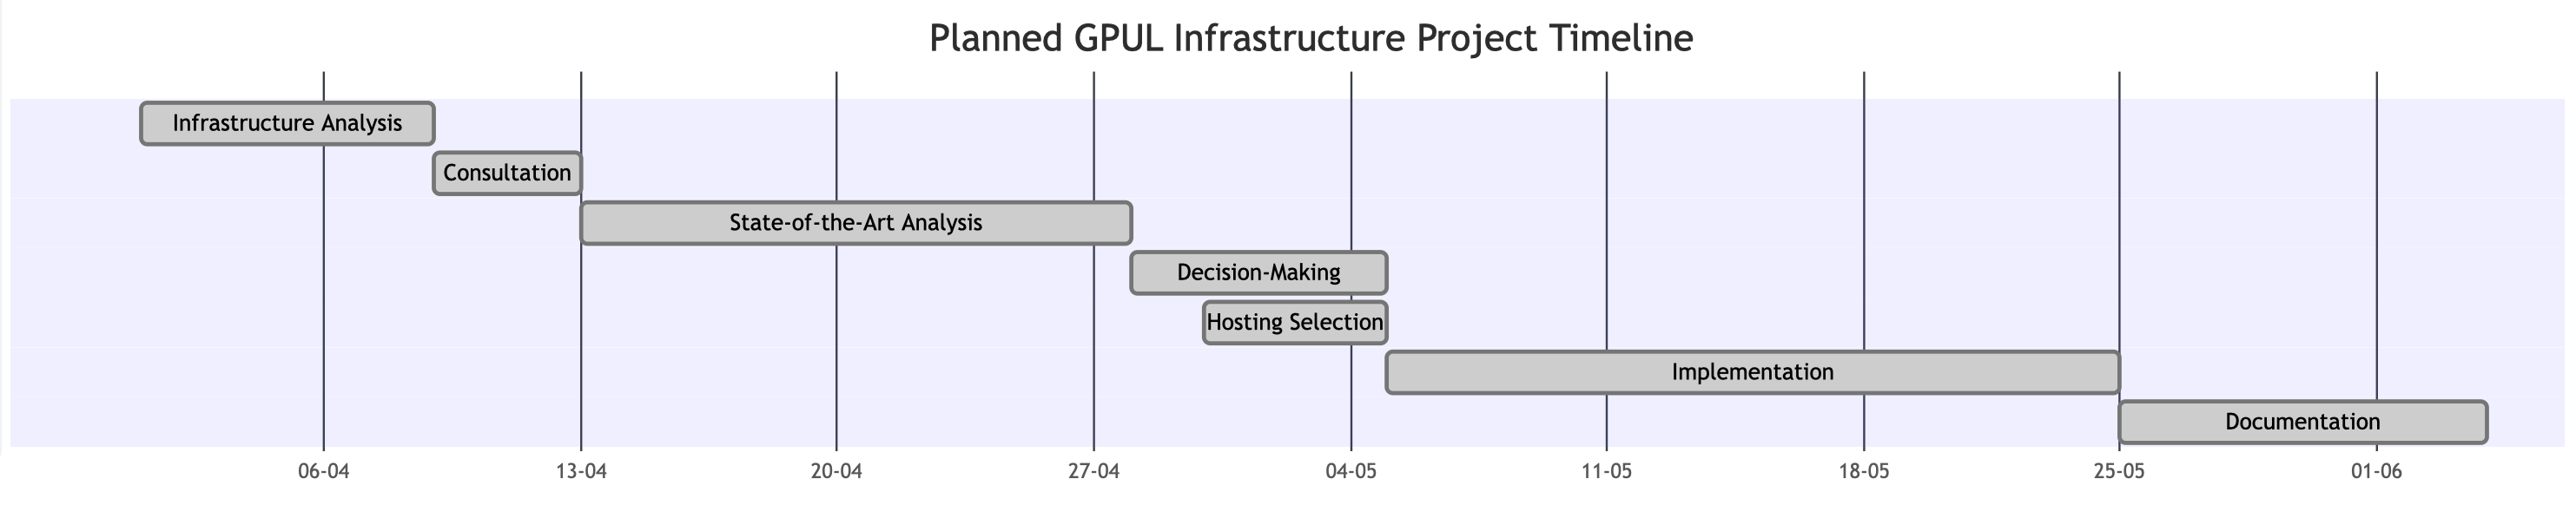
\includegraphics[width=1\textwidth]{imaxes/gantt-planned.png}
  \caption{Gantt chart illustrating the planned project phases.}
  \label{fig:gantt-planned}
\end{figure}

\subsection*{Phases}

\begin{enumerate}
  \item \textbf{Initial Infrastructure Analysis}\\
  Independent analysis of the legacy servers \texttt{GPULINO} and \texttt{GPULON}. Task included service inspection and identification of required services.\\
  \emph{Estimated duration: \(\sim 50\)~hours.}

  \item \textbf{Consultation and Requirements Gathering}\\
  Discussions with current and former board members to define required services.\\
  \emph{Estimated duration: \(\sim 20\)~hours.}

  \item \textbf{State-of-the-Art Analysis and Testing}\\
  Research of candidate solutions and practical trials on a self-hosted test environment.\\
  \emph{Estimated duration: \(\sim 60\)~hours.}

  \item \textbf{Technology Selection}\\
  Consolidation of testing results with the board and thesis supervisor to agree on the software stack.\\
  \emph{Estimated duration: \(\sim 20\)~hours.}

  \item \textbf{Hosting Provider Selection}\\
  Meetings with local providers and evaluation of alternatives. Carried out in parallel with the previous phase.\\
  \emph{Estimated duration: \(\sim 15\)~hours.}

  \item \textbf{Implementation}\\
  Sequential deployment of the new infrastructure: provisioning the environment, installing Incus, configuring containers, and deploying the selected services.\\
  \emph{Estimated duration: \(\sim 90\)~hours.}

  \item \textbf{Documentation and Thesis Writing}\\
  Documentation of procedures and preparation of the thesis document.\\
  \emph{Estimated duration: \(\sim 30\)~hours.}

\end{enumerate}

\subsection*{Relevant Deviations}

While the overall structure of the project largely followed the initial plan, several key deviations occurred, primarily impacting the project timeline. Most notably, all phases commenced approximately one week later than initially anticipated, leading to incremental delays in subsequent stages.

The primary delay arose during the hosting provider selection phase. Initial conversations suggested an imminent agreement; however, the final proposal did not meet the association's expectations in terms of value and resource allocation. This unexpected outcome necessitated reopening discussions and evaluating alternative options, significantly pushing back the start of the implementation phase.

Furthermore, work was completely halted between June 12th and 15th due to organizational duties for the AtlanticaConf event. This interruption occurred during a peak implementation period, compounding the initial delays and further extending the project timeline.

Due to these compounded delays, the implementation phase had to be adjusted. Instead of fully migrating all services immediately, a decision was made to thoroughly test and validate migration procedures, ensuring readiness without performing the complete migrations. The final domain migrations and service transitions were intentionally postponed until after this thesis submission.

To effectively facilitate this postponed migration, an already scheduled on-site retreat, originally planned for general association maintenance and fostering new ideas and future activities, was partially repurposed. This intensive weekend will now also include migration tasks, with the in-person communication enabling faster account provisioning and smoother transitions compared to the usual asynchronous exchanges. The direct face-to-face interactions will streamline knowledge transfer between current, historical, and newly active board members, avoiding the delays inherent to remote communication. Ultimately, this adjustment addressed the tight thesis submission deadline while promoting long-term infrastructure sustainability through enhanced collective involvement and communication.

Figure~\ref{fig:gantt-real} illustrates the revised project timeline, which reflects the initial one-week offset and the subsequent delays. As a result, the implementation phase extended into early July, with final migrations deferred until after the thesis submission.

\begin{figure}[H]
  \centering
  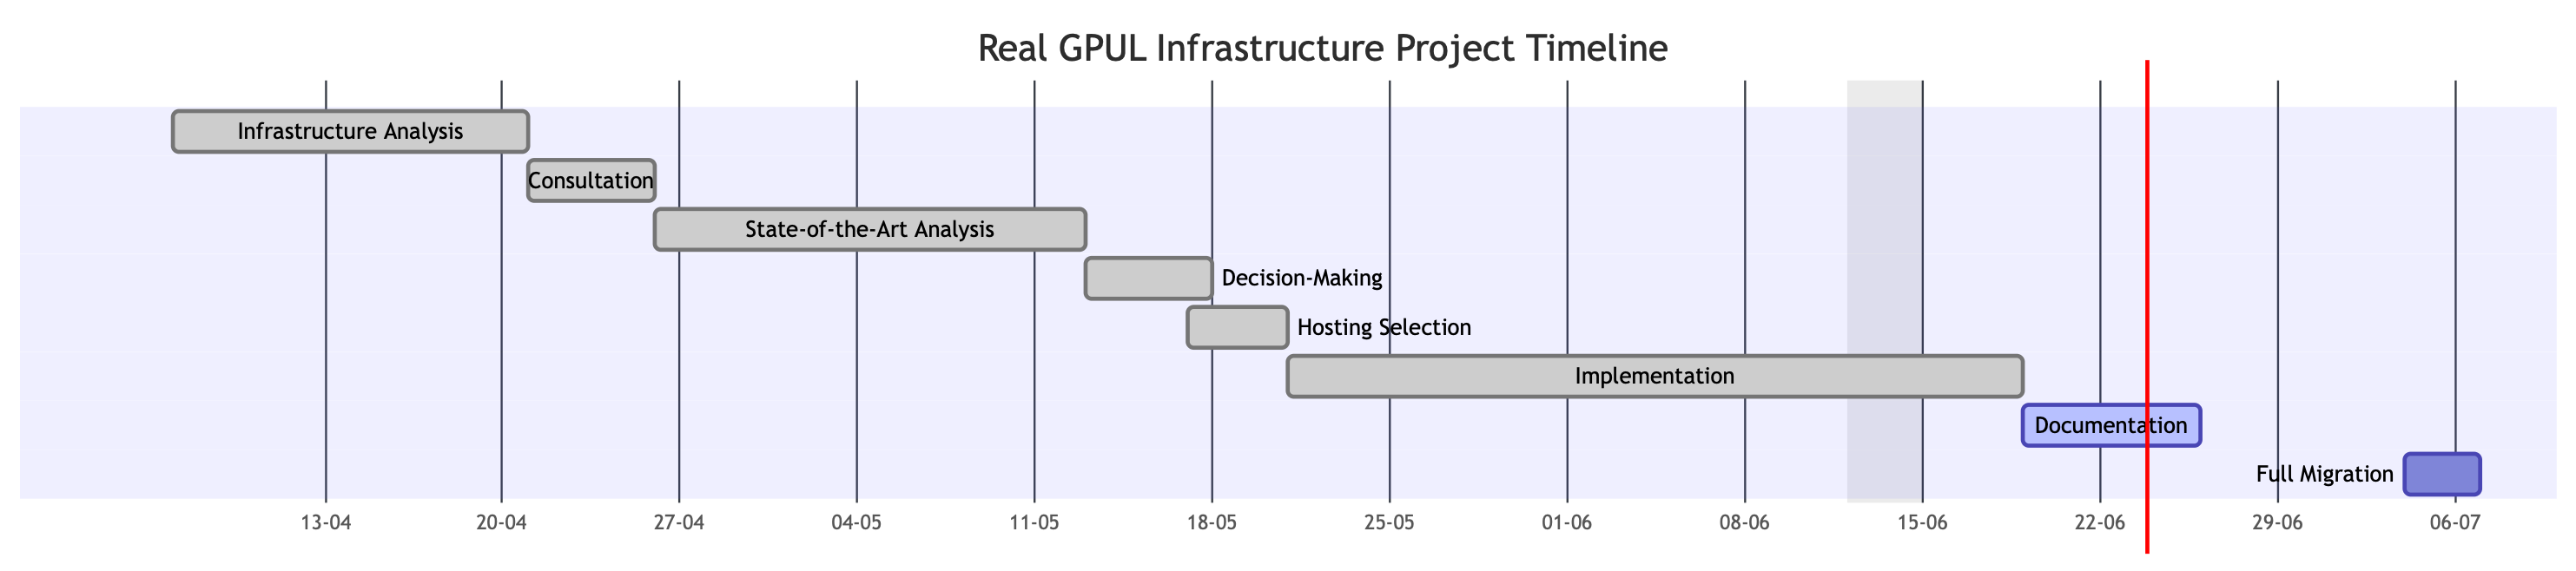
\includegraphics[width=1\textwidth]{imaxes/gantt-real.png}
  \caption{Gantt chart illustrating the real project phases.}
  \label{fig:gantt-real}
\end{figure}

\section{Cost Estimation}

Although this project was conducted under the umbrella of a volunteer-driven nonprofit organization, certain infrastructure, equipment, and labor costs can be roughly estimated to provide context on the real-world value of the work.

\subsection*{Equipment and Resources}

The development and testing work was carried out using a personal laptop and a repurposed self-hosted desktop PC:

\begin{itemize}
  \item \textbf{Laptop (development machine)}: \(\sim 1\,200€\), mid-range Linux-compatible machine.
  \item \textbf{Test server}: no acquisition cost, reused legacy hardware from prior GPUL use.
  \item \textbf{Domain name} (\texttt{gpulux.org}): \(\sim 10€\)/year.
  \item \textbf{Production server}: costs are detailed in Chapter~\ref{chap:hosting-provider}.
\end{itemize}

\subsection*{Human Resources and Labor Value}

While no direct financial compensation was involved, estimating the cost of human labor provides perspective on the real investment made, especially considering that all three individuals involved (the author and two supervisors) are not only members of the association, but also active or former board members with a high level of involvement and responsibility.

\begin{itemize}
  \item \textbf{System Administration and Infrastructure Work}: Based on the 2024 Manfred Developer Report~\cite{manfred-salary-guide}, see Figure~\ref{fig:salary-chart}, the most common salary bracket for SysAdmin roles is \textbf{€30-40K}. This work cannot be considered entry-level, as the author has over five years of professional experience and holds prior technical qualifications. Assuming a midpoint of \textbf{€35\,000} for a full-time equivalent, and with an estimated dedication of 300 hours, the work carried out corresponds to a market value of approximately \(\sim 5\,800€\).

  \item \textbf{Supervision and Guidance}: For technical supervisors involved in infrastructure or SRE roles, the most common salary bracket is higher: \textbf{€40-50K}. Using a midpoint estimate of \textbf{€45\,000} per year, their involvement (estimated 8-12 hours per supervisor) corresponds to an approximate market value of \(\sim 450€\) in total.
\end{itemize}

\begin{figure}[H]
  \centering
  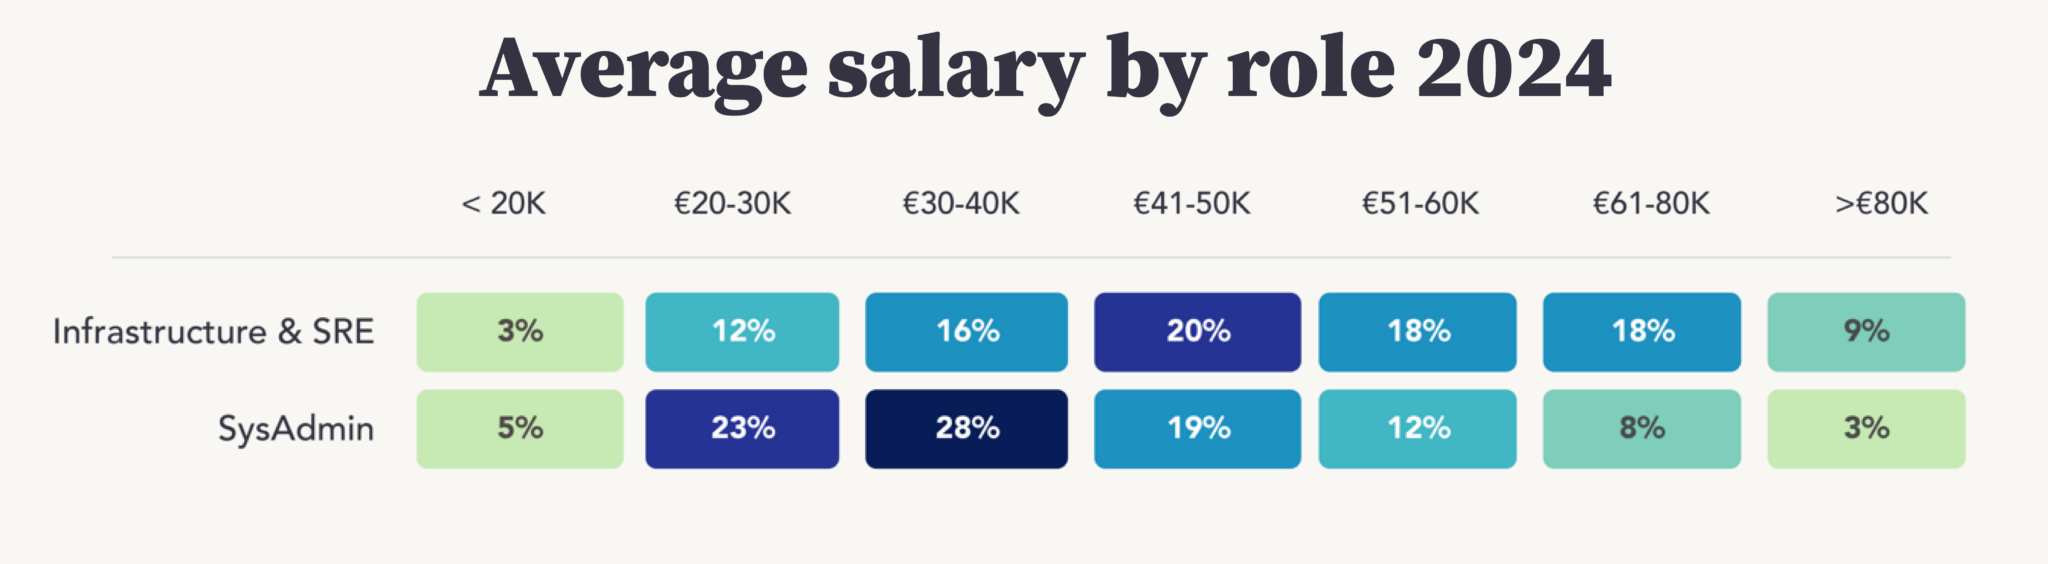
\includegraphics[width=0.8\textwidth]{imaxes/salary-chart.png}
  \caption{Average salary distribution in Spain by role.}
  \label{fig:salary-chart}
\end{figure}

These estimates illustrate that while the project was executed in a volunteer context, the real value of the technical and organizational contributions exceeds \(\sim 6\,000€\). This reinforces the importance of properly valuing community infrastructure efforts and documenting them for long-term sustainability.

  % SPDX-FileCopyrightText: 2025 Jorge Teixeira Crespo <jorge.teixeira@udc.es>
%
% SPDX-License-Identifier: GPL-2.0-or-later

\chapter{Current Infrastructure Analysis}
\label{chap:current-infrastructure}

\lettrine{A}{n} in-depth analysis of GPUL's current server infrastructure focuses on the two legacy servers: GPULINO and GPULON. These servers host critical services but also pose significant operational and maintenance challenges. GPULINO, created on November 3, 2011, and GPULON, launched on January 17, 2016, have remained largely unchanged since their deployment. The chapter reviews their specifications, configurations, and highlights key issues such as outdated software, inconsistent backup strategies, and the lack of proper documentation. It also discusses the impact of these limitations on GPUL's operations, underlining the urgent need for a comprehensive infrastructure renewal.

\section{GPULINO Server Analysis}

GPULINO is hosted with Gandi, located in their Paris, France (SD3 datacenter). It runs Debian GNU/Linux 8 (Jessie), which is significantly outdated. Its official End-of-Life (EOL) was June 17, 2018, and Long-Term Support (LTS) concluded on June 30, 2020.

\subsection*{Technical Specifications}

GPULINO is a legacy virtual machine that remains in active use within the association's infrastructure. Provisioned in 2011, it has undergone minimal changes since its deployment. The table below summarizes its key specifications, which reflect the outdated and limited nature of the system. These constraints have direct implications for performance, maintenance, and security.

\begin{table}[H]
  \centering
  \rowcolors{2}{white}{udcgray!25}
  \caption{GPULINO Server Specifications}
  \label{tab:gpulino_specs}
  \begin{tabular}{ll}
    \rowcolor{udcpink!25}
    \textbf{Specification} & \textbf{Details} \\
    \hline
    CPU & 1 core \\
    RAM & 640 MB \\
    Storage & 3 x 10 GB volumes \\
    Monthly Cost & €13.09 \\
    IPv4 & 95.142.163.196 \\
    IPv6 & 2001:4b98:dc0:47:216:3eff:fe56:1785 \\
    OS & Debian GNU/Linux 8 (Jessie, EOL) \\
  \end{tabular}
\end{table}

\subsection*{Filesystem Structure}

GPULINO uses three independent 10 GB volumes provided by the hosting provider. These are mounted as root (\verb|/|), data (\verb|/srv/srv_gpulino|), and backup (\verb|/srv/backup_gpulino|). Their current usage is visualized in Figure~\ref{fig:gpulino_disk_usage}.

\begin{figure}[H]
  \centering
  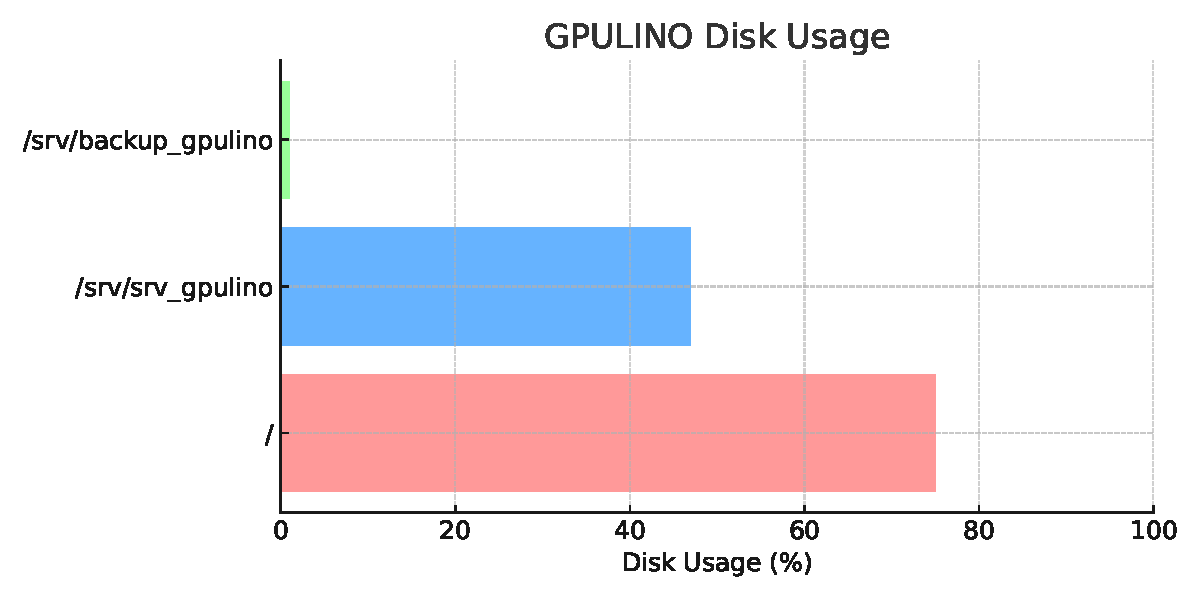
\includegraphics[width=0.7\textwidth]{figuras/gpulino_disk_usage.pdf}
  \caption{Disk usage across GPULINO volumes.}
  \label{fig:gpulino_disk_usage}
\end{figure}

While the root filesystem is nearing critical usage (~75\%), the backup volume remains largely underutilized (~1\%), showcasing the lack of backup strategy.

\subsection*{User Access and Management}

The server maintains several user accounts, with varying levels of activity. Table \ref{tab:gpulino_users} shows the most relevant user logins:

\begin{table}[H]
  \centering
  \rowcolors{2}{white}{udcgray!25}
  \caption{GPULINO Active User Accounts (sorted by creation date)}
  \label{tab:gpulino_users}
  \begin{tabular}{ll}
    \rowcolor{udcpink!25}
    \textbf{Username} & \textbf{Last Login} \\
    \hline
    adm***** & September 26, 2020 \\
    tsa***** & September 27, 2024 \\
    ssa***** & January 27, 2024 \\
    mar***** & February 19, 2014 \\
    cas***** & March 18, 2017 \\
    che***** & April 24, 2019 \\
    tei***** & January 19, 2025 \\
  \end{tabular}
\end{table}

\subsection*{Active Services and Usage Details}

The server hosts several critical services:
\begin{itemize}
    \item Apache2 Web Server
    \item Exim4 Mail Transport Agent
    \item Mailman 2 (for mailing lists)
    \item MySQL (database server, supporting Mailman)
    \item SSH (Secure Shell)
\end{itemize}

Although these services were known to be active, GPULINO lacked formal documentation. A manual inspection of the server's filesystem and configuration files revealed various hosted domains, tools, and historical content.

The Apache configuration included several virtual hosts pointing to subdomains, some of which were no longer functional. Others still displayed static content or redirected to internal projects.

\begin{table}[H]
  \centering
  \rowcolors{2}{white}{udcgray!15}
  \caption{Web domains served by Apache on GPULINO}
  \label{tab:gpulino_apache_domains}
  \begin{tabular}{ll}
    \rowcolor{udcpink!25}
    \textbf{Domain} & \textbf{Notes} \\
    \hline
    \texttt{planet.gpul.org} & Hosts a blog or webpage \\
    \texttt{old.gpul.org} & Returns a PHP error \\
    \texttt{stuff.gpul.org} & Hosts a webpage \\
    \texttt{dudesconf.org} & Hosts a webpage (some links broken) \\
    \texttt{junoffice.gpul.org} & Returns an empty page \\
    Other domains & Serve the default Apache welcome page \\
  \end{tabular}
\end{table}

These domains pointed to directories inside \texttt{/var/www}, which contained a variety of static and symlinked content likely tied to past events, services, or internal documentation.

\begin{table}[H]
  \centering
  \rowcolors{2}{white}{udcgray!15}
  \caption{Apache web directories found under \texttt{/var/www}}
  \label{tab:gpulino_www_dirs}
  \begin{tabular}{ll}
    \rowcolor{udcpink!25}
    \textbf{Directory} & \textbf{Description} \\
    \hline
    apache-default & Default Apache content \\
    artwork & Publicly accessible artwork files \\
    drupal & Linked to \texttt{/var/www/gpul.org/drupal} \\
    dudesconf & Hosts content for dudesconf.org \\
    estatutos & Organizational rules or statutes \\
    etherpad-lite & Likely collaborative editor \\
    eventostuff & Linked to \verb|/srv/srv_gpulino/eventos| \\
    gallery2 & Public gallery \\
    gpul-latex & LaTeX-related files \\
    gpul.org & Main content for GPUL \\
    gpul.org-eventos & Event-specific content \\
    guademy & Linked to \verb|/srv/srv_gpulino/www/guademy/| \\
    indico & Linked to \verb|/srv/srv_gpulino/indico| \\
    junoffice & Content for junoffice.gpul.org \\
    labs.gpul.org & Lab-related subdomain \\
    piwik & Web analytics platform \\
    planet.gpul.org & Static site content \\
    rexistro.labs.gpul.org & Registry or logs \\
    votologo & Likely a voting tool \\
  \end{tabular}
\end{table}

Mailman was configured to manage mailing lists under the \texttt{lists.gpul.org} domain, using a CGI interface and Apache redirection rules. The configuration was minimal but functional.

\begin{table}[H]
  \centering
  \rowcolors{2}{white}{udcgray!15}
  \caption{Mailman service details on GPULINO}
  \label{tab:gpulino_mailman}
  \begin{tabular}{ll}
    \rowcolor{udcpink!25}
    \textbf{Parameter} & \textbf{Value} \\
    \hline
    Domain & \texttt{lists.gpul.org} \\
    VirtualHost & Redirects root to \texttt{/cgi-bin/mailman/listinfo} \\
    CGI Path & \texttt{/usr/lib/cgi-bin/} \\
    DocumentRoot & \texttt{/var/www/} \\
    Admin Email & \texttt{mailman@lists.gpul.org} \\
  \end{tabular}
\end{table}

The server also ran a Git daemon that served multiple repositories under a single base path. These were accessible via the \texttt{git://} protocol and configured to run from a root-owned script.

\begin{table}[H]
  \centering
  \rowcolors{2}{white}{udcgray!15}
  \caption{Git daemon configuration details}
  \label{tab:gpulino_git_daemon}
  \begin{tabular}{ll}
    \rowcolor{udcpink!25}
    \textbf{Parameter} & \textbf{Value} \\
    \hline
    Startup Script & \texttt{/root/git-daemon} \\
    Base Path & \verb|/srv/srv_gpulino/git/repositories/| \\
  \end{tabular}
\end{table}

\noindent
\textbf{Git Daemon Command:}

\begin{lstlisting}[language=sh]
/usr/bin/git-daemon \
  --user=git --group=git \
  --verbose \
  --reuseaddr \
  --base-path=/srv/srv_gpulino/git/repositories/ \
  /srv/srv_gpulino/git/repositories/
\end{lstlisting}

\begin{table}[H]
  \centering
  \rowcolors{2}{white}{udcgray!15}
  \caption{Git repositories hosted}
  \label{tab:gpulino_git_repos}
  \begin{tabular}{ll}
    \rowcolor{udcpink!25}
    \textbf{Repository} & \textbf{Description} \\
    \hline
    \texttt{actas.git} & Meeting minutes \\
    \texttt{certificado-asistencia.git} & Attendance certificates \\
    \texttt{cuentas.git} & Financial records \\
    \texttt{gitosis-admin.git} & Git access management \\
    \texttt{gpul-estatutos.git} & Organization statutes \\
    \texttt{manual-latex.git} & LaTeX training material \\
    \texttt{mem-dudesconf.git} & DudesConf report \\
    \texttt{parte-gasto.git} & Expense reports \\
    \texttt{subvencion-udc-2011.git} & UDC grant files (2011) \\
  \end{tabular}
\end{table}

These findings illustrate the range of active uses the server had, many of which were not documented but still functional at the time of analysis. They also reflect the historical depth and variety of GPUL's activities over the years.

\section{GPULON Server Analysis}

GPULON is hosted with Kimsufi and configured as a KS-4C server running Debian GNU/Linux 11 (Bullseye).

\subsection*{Technical Specifications}

\begin{table}[H]
  \centering
  \rowcolors{2}{white}{udcgray!25}
  \caption{GPULON Server Specifications}
  \label{tab:gpulon_specs}
  \begin{tabular}{ll}
    \rowcolor{udcpink!25}
    \textbf{Specification} & \textbf{Details} \\
    \hline
    CPU & Intel i5-2300 \\
    RAM & 16 GB \\
    Storage & 1 x 2TB HDD \\
    Monthly Cost & €30.60 \\
    IPv4 & 91.121.65.91 \\
    OS & Debian GNU/Linux 11 (Bullseye) \\
  \end{tabular}
\end{table}

\subsection*{Filesystem Structure}

GPULON has a single 2 TB physical disk, divided into logical volumes for \texttt{/home}, \texttt{/var/lib/docker}, and the root filesystem (\texttt{/}). This setup is visualized in Figure~\ref{fig:gpulon_disk_usage}.

\begin{figure}[H]
  \centering
  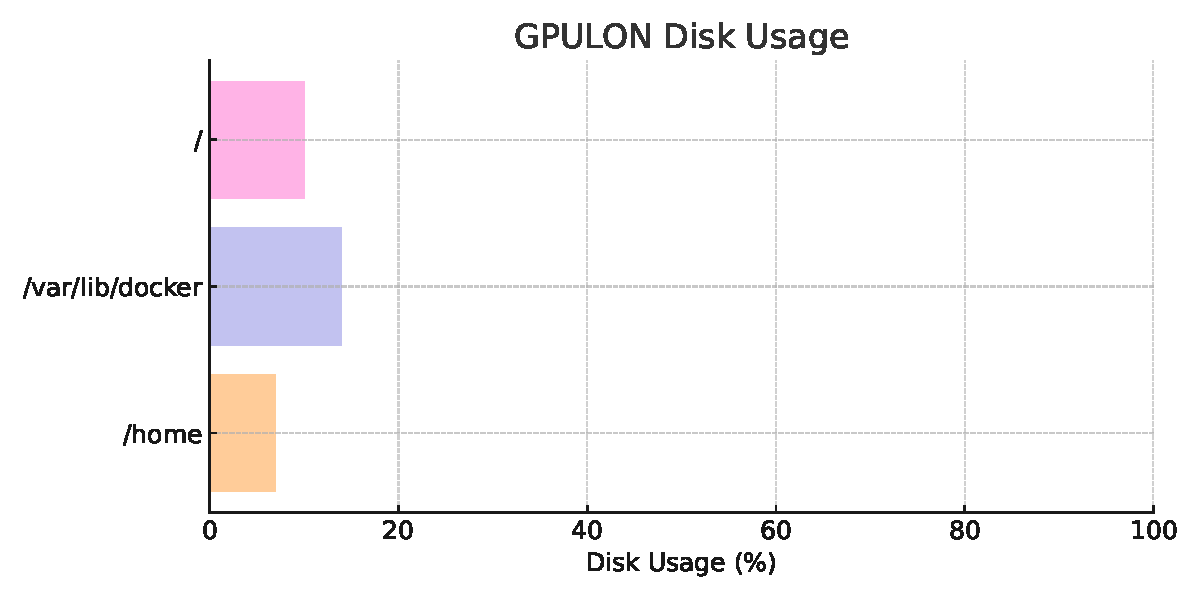
\includegraphics[width=0.7\textwidth]{figuras/gpulon_disk_usage.pdf}
  \caption{Disk usage across GPULON logical volumes after reallocation.}
  \label{fig:gpulon_disk_usage}
\end{figure}

Originally, the Docker directory (\texttt{/var/lib/docker}) had been restricted to approximately 450 GB and became rapidly saturated, primarily due to logs generated by long-running containerized services. One Nextcloud log file alone exceeded 250 GB.

This issue caused an operational incident that affected system stability. Resolving it involved manually deleting the oversized log and reallocating disk space to expand the Docker volume.

The updated logical volume allocation now stands as follows:

\begin{itemize}
    \item \texttt{/home} — 272 GB (7\% usage)
    \item \texttt{/var/lib/docker} — 1.5 TB (14\% usage)
    \item Root filesystem (\texttt{/}) — 58 GB (10\% usage)
\end{itemize}

This reallocation has significantly improved headroom for service logs and application data, reducing the risk of similar incidents in the future.

\subsection*{User Access and Management}

Table \ref{tab:gpulon_users} shows the active user accounts on GPULON:

\begin{table}[H]
  \centering
  \rowcolors{2}{white}{udcgray!25}
  \caption{GPULON Active User Accounts (sorted by creation date)}
  \label{tab:gpulon_users}
  \begin{tabular}{ll}
    \rowcolor{udcpink!25}
    \textbf{Username} & \textbf{Last Login} \\
    \hline
    roo***** & January 17, 2016 \\
    ssa***** & April 1, 2025 \\
    cas***** & September 25, 2020 \\
    dav***** & August 22, 2023 \\
    bru***** & August 9, 2024 \\
    tsa***** & October 1, 2023 \\
    ped***** & March 27, 2022 \\
    tei***** & May 17, 2025 \\
    del***** & March 29, 2025 \\
  \end{tabular}
\end{table}

\subsection*{Docker Environment}

GPULON primarily uses Docker for service deployment, hosting:
\begin{itemize}
  \item Nextcloud (cloud suite platform)
  \item Listmonk (email marketing platform)
  \item Activepieces (automation platform)
  \item Traefik (reverse proxy)
  \item Various supporting databases (Postgres, Redis, MariaDB)
\end{itemize}

\section{Critical Issues and Challenges}

Although GPUL's servers are still running, they have many problems that make them hard to maintain and unreliable. Over time, different people have made changes without clear planning or documentation, which has led to a fragile system. This section describes the main problems we found, divided into two groups: serious issues that affect how the servers work, and general problems with how the infrastructure is set up.

\subsection*{Known Critical Issues}

The current infrastructure presents several critical issues:
\begin{itemize}
  \item \textbf{OS Obsolescence}: GPULINO is severely outdated, running an EOL operating system.
  \item \textbf{Nextcloud Obsolescence}: The Nextcloud version used is 24.0.6, which is no longer maintained. The latest is version 31.
  \item \textbf{Manual Interventions}: Critical services require manual restart post-reboot.
  \item \textbf{Insufficient Backup Strategy}: No systematic backup; sporadic manual backups to personal NAS.
  \item \textbf{Lack of Automated Log Rotation}: Manual log maintenance required, causing periodic instability.
\end{itemize}

\subsection*{Known Infrastructure Issues}

Additional challenges include:
\begin{itemize}
  \item \textbf{Docker Misconfiguration (GPULON)}: The \texttt{/srv/docker} directory has grown into a chaotic collection of loosely organized folders and services, with multiple Docker Compose files scattered across subdirectories in inconsistent ways. There is little to no documentation, naming is irregular, and services are grouped without a clear structure, making it extremely difficult to understand what is running or how components are connected.
  \item \textbf{Unknown Installed Services (GPULINO)}: Legacy services were poorly documented, making it difficult to determine what was hosted or how services were configured. Understanding the system required inspection of configuration files, web directories, and service logs, effectively a detailed forensic review akin to a forensic investigation.
\end{itemize}

\section{Impact on Operations}

GPUL's current infrastructure has already caused serious disruptions to the organization's daily operations. These issues are not only technical, they affect how GPUL communicates, plans events, and meets important deadlines. A clear example of this is the ongoing trouble with the email system. GPUL uses redirects for several critical email addresses under the \texttt{gpul.org} domain. However, this setup often causes messages to be marked as spam. As a result, important emails related to event organization, sponsors, or participants are sometimes not delivered or go unnoticed, making coordination much harder.

Another major incident occurred when the GPULON server became unresponsive due to unrotated log files completely filling up the server's disk. This failure happened just before the end of a financial quarter, a key moment for administrative tasks. Resolving the issue took four days, required assistance from the external hosting provider, and placed GPUL at risk of missing key reporting deadlines. This event highlighted the fragility and poor maintainability of the current system, and how technical problems can quickly become organizational ones.

  % SPDX-FileCopyrightText: 2025 Jorge Teixeira Crespo <jorge.teixeira@udc.es>
%
% SPDX-License-Identifier: GPL-2.0-or-later

\chapter{State of the Art}
\label{chap:state-of-the-art}

\lettrine{T}{he} following sections survey the principal technical options for each core service GPUL operates or is expected to adopt in the near future.  
For every category an introduction explains its relevance, followed by one \emph{Current stack} subsection and a set of numbered subsections that describe the state of the art.  

%--------------------------------------------------------------------
\section{Mailing-list Managers}

\textbf{Importance.} Mailing lists are a foundational tool for formal communication, providing a standardized and archivable channel for discussions and announcements. For community-driven associations, they are crucial for transparent decision-making and record-keeping. This is especially true for GPUL, as its statutes explicitly name mailing lists as the official communication channel. Consequently, the service must be reliable, searchable, and permanently archived to preserve organizational history and ensure newcomers can access past discussions.

\subsection*{Current stack}
\textbf{Mailman 2} running on Debian 8 (see Figure~\ref{fig:mailman2}).

\begin{figure}[h!]
  \centering
  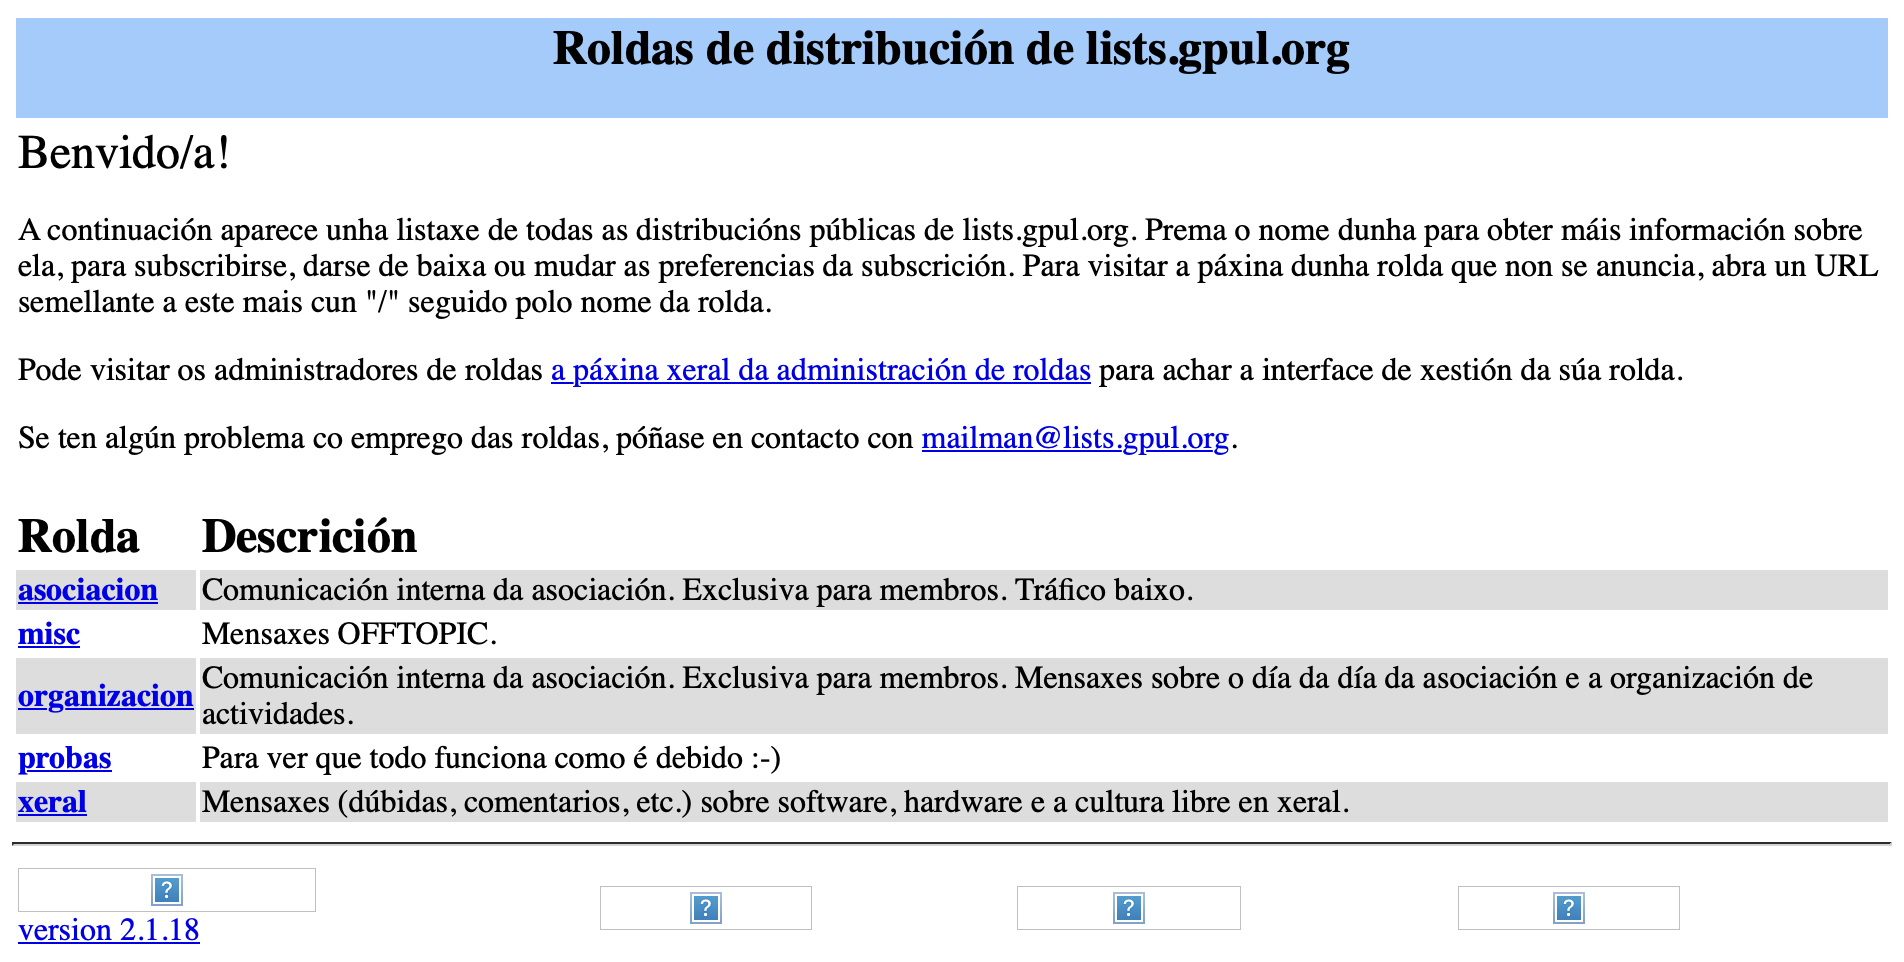
\includegraphics[width=0.9\textwidth]{imaxes/mailman-2-current.png}
  \caption{Screenshot of the Mailman 2 web interface currently in use}
  \label{fig:mailman2}
\end{figure}

\subsection*{Mailman 3 + HyperKitty}

Mailman~3 is a modular mailing list management system, described in its official documentation~\cite{mailman-install-docs}. It is the modern successor to the Mailman~2 software currently in use, and includes official migration tools to assist in upgrading existing lists and archives. Its core component, Mailman Core, is responsible for all mailing list logic and message delivery. It communicates with a Mail Transfer Agent (MTA) via \gls{lmtp} for incoming messages and \gls{smtp} for outgoing ones, and exposes a \gls{restapi} for external interfaces.

HyperKitty~\cite{hyperkitty-docs} is the web-based archiver of Mailman~3, designed to replace Pipermail. It receives messages from Mailman Core through the \texttt{mailman-hyperkitty} plugin and indexes them into a database. The messages are then accessible via a modern web interface that allows browsing, searching, and replying to threads.

While Postorius~\cite{postorius-docs} is often deployed alongside HyperKitty as part of the Mailman suite, it is not required for operation. Postorius provides a web interface for managing mailing lists, users, and settings, serving as a frontend to the \gls{restapi}. However, these tasks can also be performed using the command-line tools or direct API calls.

All components of the Mailman~3 project are fully open source and licensed under the GNU General Public License (GPL), aligning with the principles of this work.

\subsection*{Sympa 7}

Sympa (version~7) is a free and open-source mailing list manager licensed under the GNU General Public License (GPL)~\cite{sympa-docs}. It is designed for scalability and flexibility, featuring a modular architecture with dedicated daemons for each task and a relational database backend. Sympa supports advanced functionality such as virtual hosting, bounce management, message archiving, and fine-grained access control.

Its web interface (WWSympa) allows users and administrators to manage subscriptions, review moderation queues, and browse archives. The software is widely used by universities and research institutions, and aligns with the principles of this work thanks to its self-hosted, open-source nature. A screenshot of the interface is shown in Figure~\ref{fig:sympa}.

\begin{figure}[h!]
  \centering
  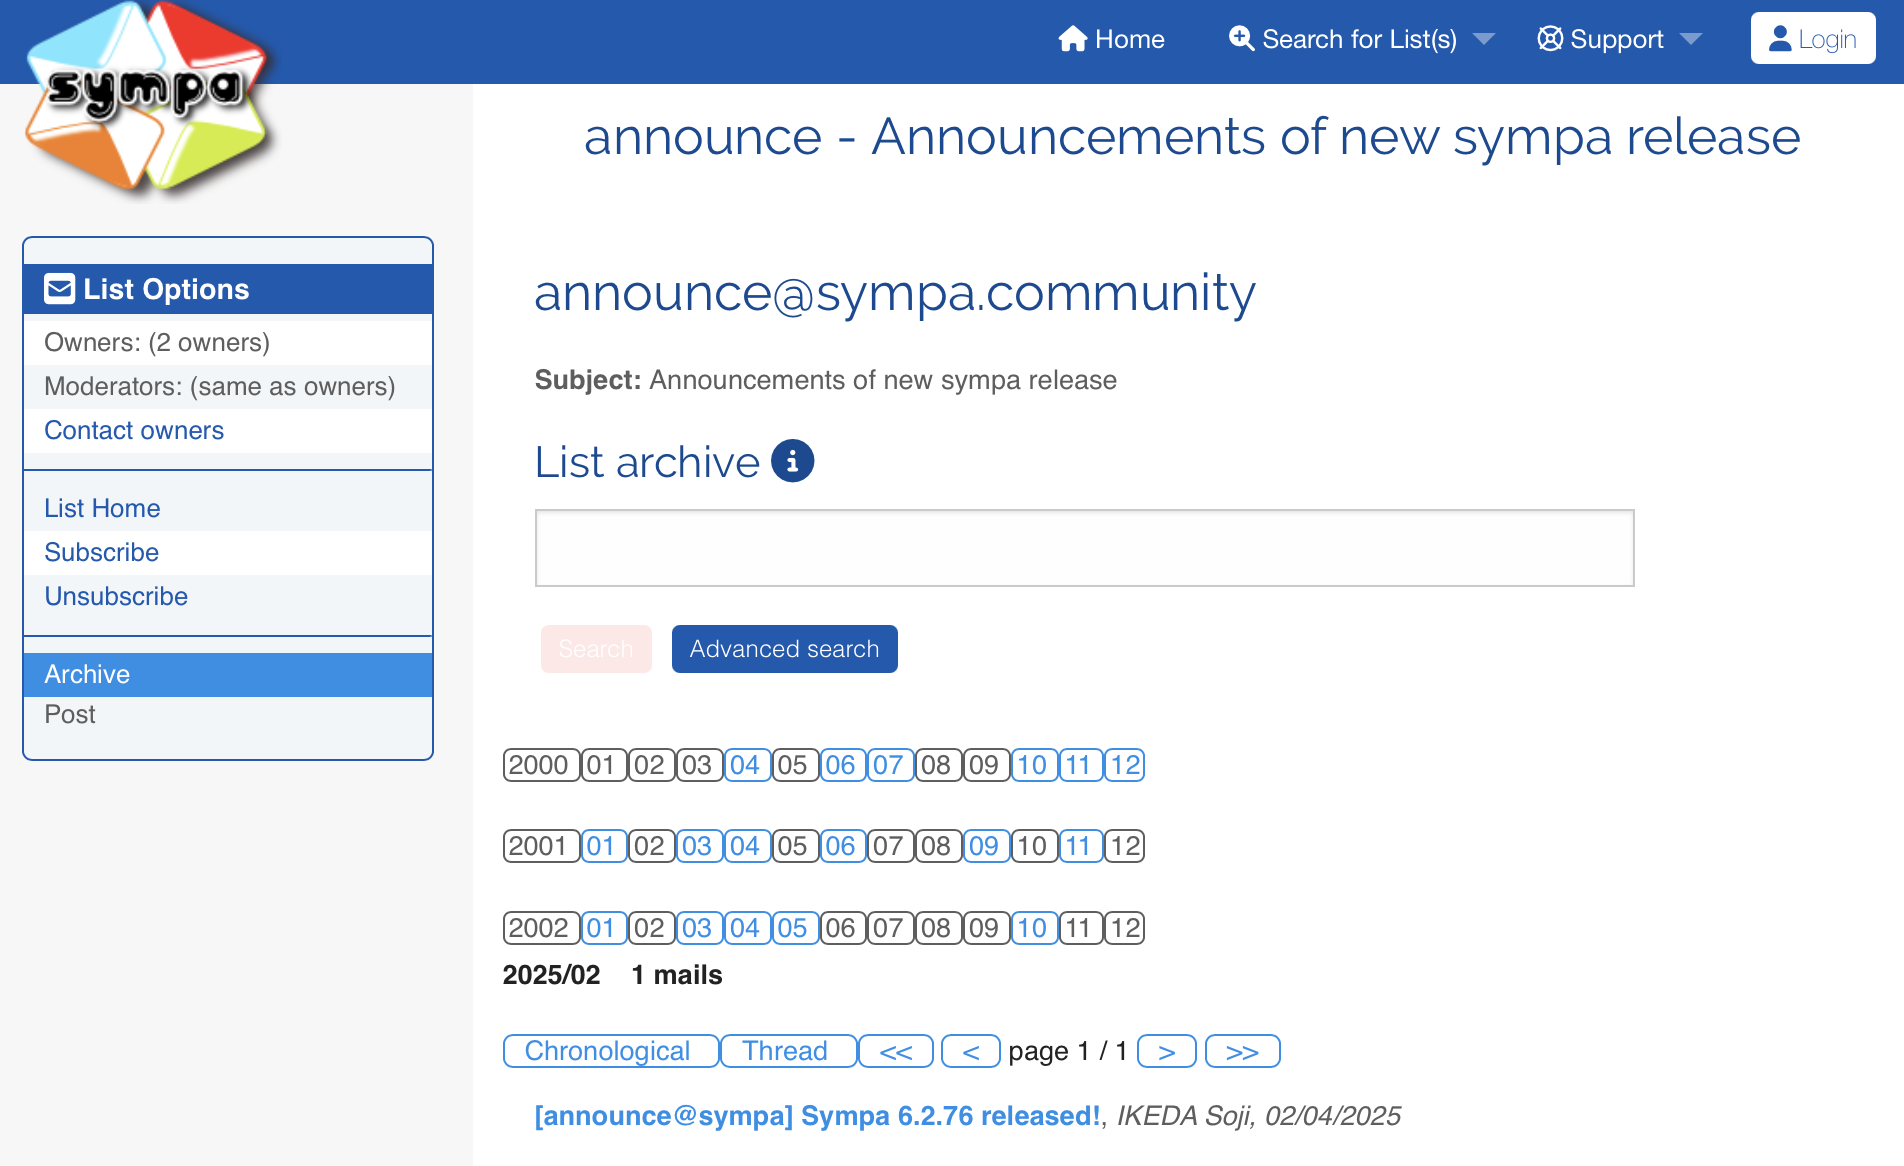
\includegraphics[width=0.9\textwidth]{imaxes/sympa.png}
  \caption{Screenshot of the Sympa 7 mailing list interface}
  \label{fig:sympa}
\end{figure}

\subsection*{Google Groups}

Google Groups is a proprietary cloud-based mailing list and discussion service provided by Google~\cite{google-groups-docs}. It allows users to create and manage groups through a web interface, with seamless integration into the broader Google ecosystem. Due to its low administrative overhead and ease of use, it has become a widely adopted tool for informal and professional communication.

However, as a closed platform, it does not support self-hosting, customization, or full data ownership. This makes it unsuitable for privacy-conscious organizations or those with a strong preference for open-source infrastructure. Despite its limitations, Google Groups is considered in this comparison due to its mainstream adoption and minimal maintenance requirements, which may appeal to less technical communities.

%--------------------------------------------------------------------
\section{Cloud Storage / Groupware}

\textbf{Importance.} Cloud storage and groupware platforms are vital for modern organizations to manage internal documents, collaborate on projects, and streamline administrative workflows. They provide a single source of truth, ensuring data is secure and accessible to authorized members. For GPUL, this service is mission-critical as it currently hosts all administrative paperwork and invoicing. Continuity of service and granular access control are therefore essential to protect sensitive data and maintain operational stability.

\subsection*{Current stack}
\textbf{Nextcloud 24 Hub 6} deployed via Docker Compose.

\subsection*{Nextcloud Hub 10 (≈ v31)}

Nextcloud Hub 10, also known as version~31, is the latest major release of the Nextcloud platform and the direct successor to the version currently in use at GPUL. It is a self-hosted groupware solution licensed under the GNU Affero General Public License (AGPL)~\cite{nextcloud-docs}. The platform offers file storage and sharing, collaborative document editing (via OnlyOffice or Collabora), calendar and contact management, video calls, and additional features through an extensible app ecosystem.

Version~10 introduces performance improvements, including faster file uploads, optimized resource usage, and integration enhancements across components such as Files, Talk, Mail, and Calendar~\cite{nextcloud-blog}. It supports user and group management, LDAP and SSO authentication, and synchronization clients for desktop and mobile platforms. A screenshot of the interface is shown in Figure~\ref{fig:nextcloud-ui}.

\begin{figure}[h!]
  \centering
  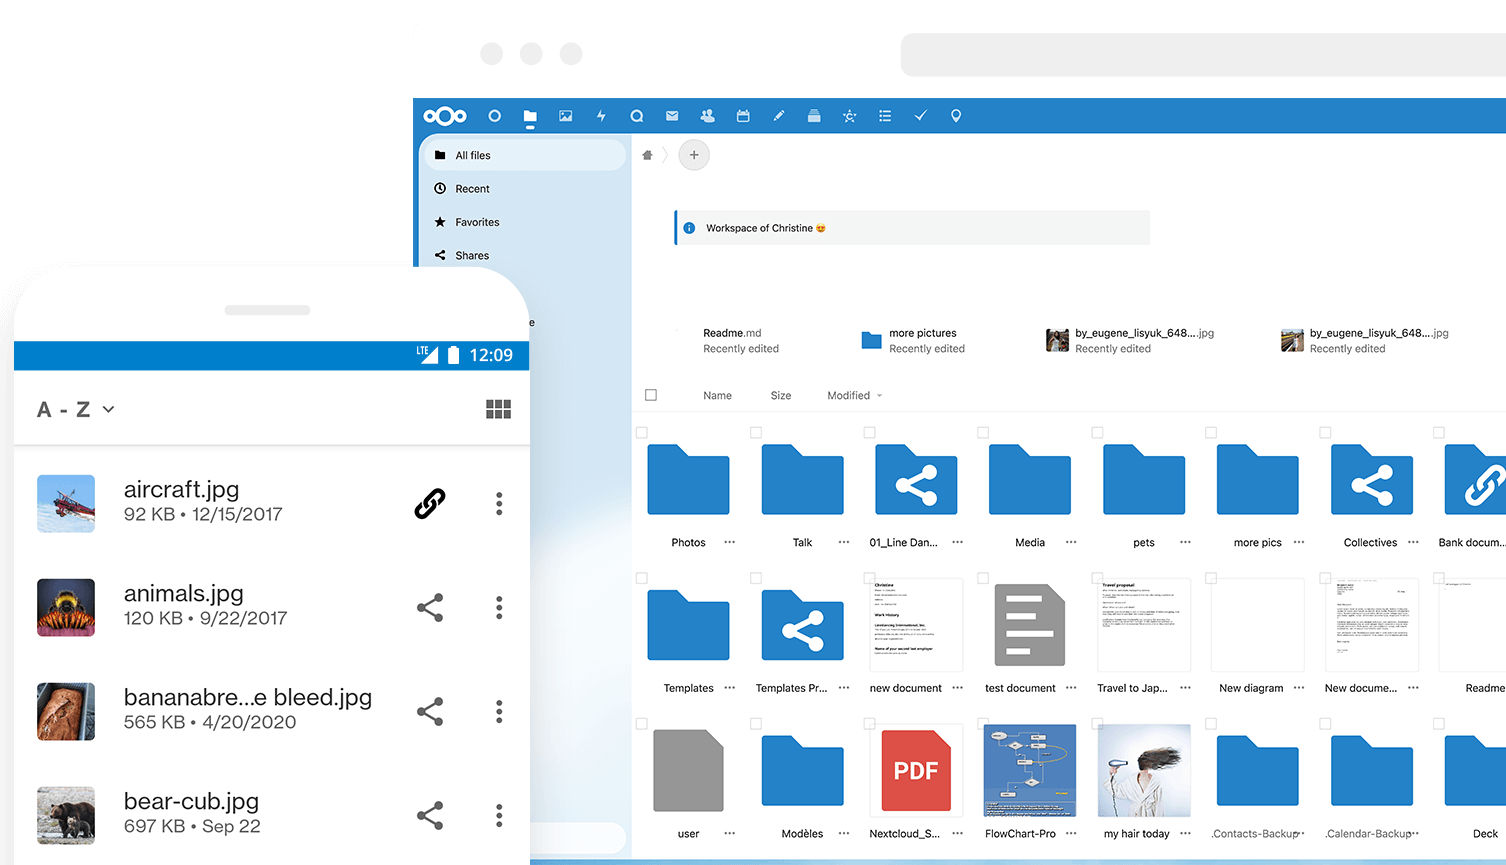
\includegraphics[width=0.9\textwidth]{imaxes/nextcloud-ui.png}
  \caption{Screenshot of the Nextcloud Hub 10 user interface}
  \label{fig:nextcloud-ui}
\end{figure}

\subsection*{ownCloud Infinite Scale}

ownCloud Infinite Scale (oCIS) is a reimplementation of the original ownCloud platform, developed as a high-performance cloud-native system written in Go~\cite{owncloud-docs}. It is licensed under the Apache License 2.0 and uses a microservices-based architecture. The system includes file synchronization and sharing, metadata management, user and role handling, and support for external storage backends~\cite{owncloud-news}.

ownCloud is the original project on which Nextcloud is based; Nextcloud was created in 2016 as a community fork of ownCloud with a separate governance and development model. oCIS introduces a redesigned backend and frontend stack, with support for container-based deployments, file firewall rules, and extended authentication options.

\subsection*{Seafile 11}

Seafile is a self-hosted file synchronization and sharing solution available under a dual license model. The Community Edition is licensed under the GNU General Public License version~3 (GPLv3), while the Professional Edition includes additional enterprise features under a commercial license~\cite{seafile-docs}. Seafile uses a content-addressable storage backend and is optimized for high performance and low latency file syncing.

Version~11 adds collaborative document editing functionality via SeaDoc, along with enhancements to its role-based access control, encryption support, and audit logging capabilities~\cite{seafile-forum}. It includes clients for desktop and mobile platforms, and supports LDAP integration.

\subsection*{Proprietary Alternatives}

Proprietary cloud storage and collaboration services such as Google Drive, Dropbox, and Microsoft 365 are widely used across various sectors. These platforms offer file sharing, document editing, and communication tools delivered as Software-as-a-Service (\gls{saas}). They are not self-hostable and operate on third-party infrastructure, with licensing and usage conditions defined by the service providers.

%--------------------------------------------------------------------
\section{Video Conferencing Platforms}

\textbf{Importance.} Video conferencing is an indispensable tool for modern collaboration, enabling remote meetings, webinars, and virtual events. For associations, it connects geographically dispersed members and facilitates engagement with external speakers and partners. This is particularly relevant for GPUL's collaboration with external participants. A self-hosted platform would not only streamline remote coordination but also align with the association's values by ensuring data sovereignty, privacy, and a consistent, professional experience when managing meetings.

\subsection*{Current stack}

GPUL currently does not operate its own video conferencing infrastructure. Meetings are typically held using platforms chosen by external participants—most commonly Google Meet or Microsoft Teams. For internal discussions, informal coordination is sometimes done via Discord or public instances of Jitsi Meet.

\subsection*{Jitsi Meet}

Jitsi Meet is an open-source video conferencing platform licensed under the Apache 2.0 License~\cite{jitsi-docs}. It uses WebRTC and a Selective Forwarding Unit (SFU) called Jitsi Videobridge to route media between participants. An XMPP server (Prosody) handles signaling, and optional components such as Jibri enable recording and live streaming. A screenshot of the interface is shown in Figure~\ref{fig:jitsi-ui}.

\begin{figure}[h!]
  \centering
  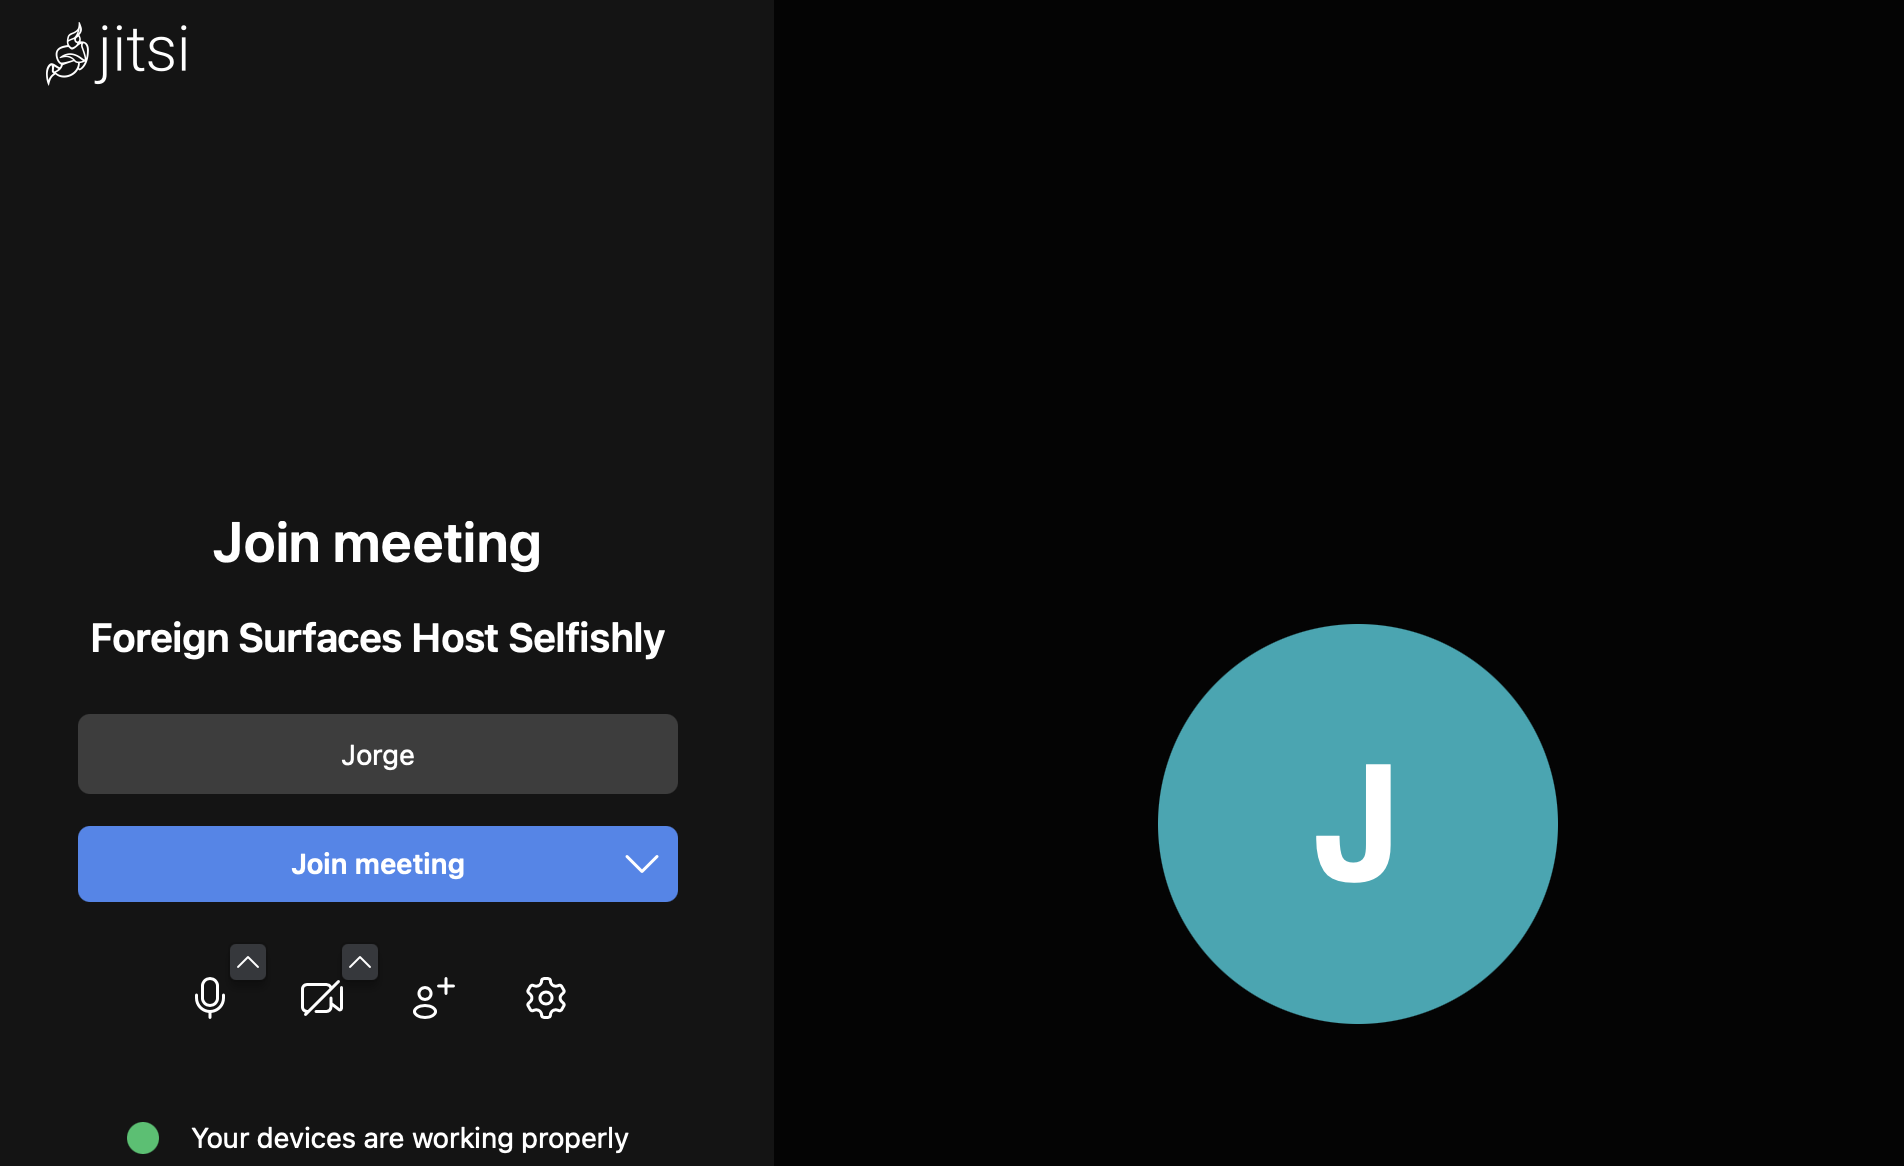
\includegraphics[width=0.9\textwidth]{imaxes/jitsi-ui.png}
  \caption{Screenshot of the Jitsi Meet interface}
  \label{fig:jitsi-ui}
\end{figure}

Features include browser-based access (no registration needed), screen sharing, in-call chat, moderation tools, and integration APIs. Jitsi can be self-hosted or used via public instances such as \texttt{meet.jit.si}.

\subsection*{BigBlueButton}

BigBlueButton is a conferencing platform optimized for online learning and released under the LGPL-3.0 License~\cite{bigbluebutton-docs}. It includes tools such as whiteboards, shared notes, polling, breakout rooms, and slide presentations. Recordings can be made and replayed in a web interface.

Its architecture combines WebRTC (via mediasoup), FreeSWITCH (for audio), and multiple backend services including Redis and Node.js. It requires significant system resources, making it more suitable for educational or high-capacity deployments.

\subsection*{Nextcloud Talk}

Nextcloud Talk is the communication module within the Nextcloud suite, licensed under the AGPL-3.0~\cite{nextcloud-talk-docs}. It offers one-on-one or group video calls, guest invitations, screen sharing, and chat, with end-to-end encryption.

Talk uses WebRTC for peer-to-peer connections and supports a High Performance Backend (HPB) for scalable multiparty calls via an SFU and signaling server. Integration with Nextcloud Hub 10 adds features such as calendar scheduling, file sharing, and federated chat and calls across Nextcloud instances. As GPUL already uses Nextcloud, Talk is interoperable with the existing stack.

\subsection*{Proprietary Alternatives}

Proprietary services such as Google Meet, Zoom, Microsoft Teams, and Cisco Webex are commonly used and offer feature-rich conferencing. However, they are not open-source and operate on third-party infrastructure, which raises concerns about data control and compliance. For this reason, they are not deeply explored.
%--------------------------------------------------------------------
\section{Git Forges}

\textbf{Importance.} A Git forge is a collaborative hub for software development, providing essential tools like issue tracking, pull requests, and CI/CD. For community-driven projects, a user-friendly forge is crucial for lowering the barrier to entry and streamlining contributor workflows. While not every association develops software, it is a key activity for GPUL. A modern forge is therefore essential to ease contributor onboarding and consolidate development, moving beyond the limitations of a legacy \texttt{git daemon}.

\subsection*{Current stack}
The current setup combines a legacy \verb|git daemon| exposed over SSH and HTTP with GitHub repositories. Most active development and contribution workflows have migrated to GitHub, while the \texttt{git daemon} continues to serve inactive older repositories.

\subsection*{Gitea 1.23 and Forgejo}

Gitea is an open-source Git forge licensed under the MIT license~\cite{gitea-docs}, designed for self-hosted deployment. It provides Git repository hosting with features such as issue tracking, pull requests, project wikis, Kanban boards, and integrated \gls{cicd} via Gitea Actions. Forgejo is a community-driven fork of Gitea initiated in 2022, also under the MIT license~\cite{forgejo-docs}. Both platforms share the same core functionality and user experience.

A screenshot of the Gitea interface is shown in Figure~\ref{fig:gitea-ui}.

\begin{figure}[h!]
  \centering
  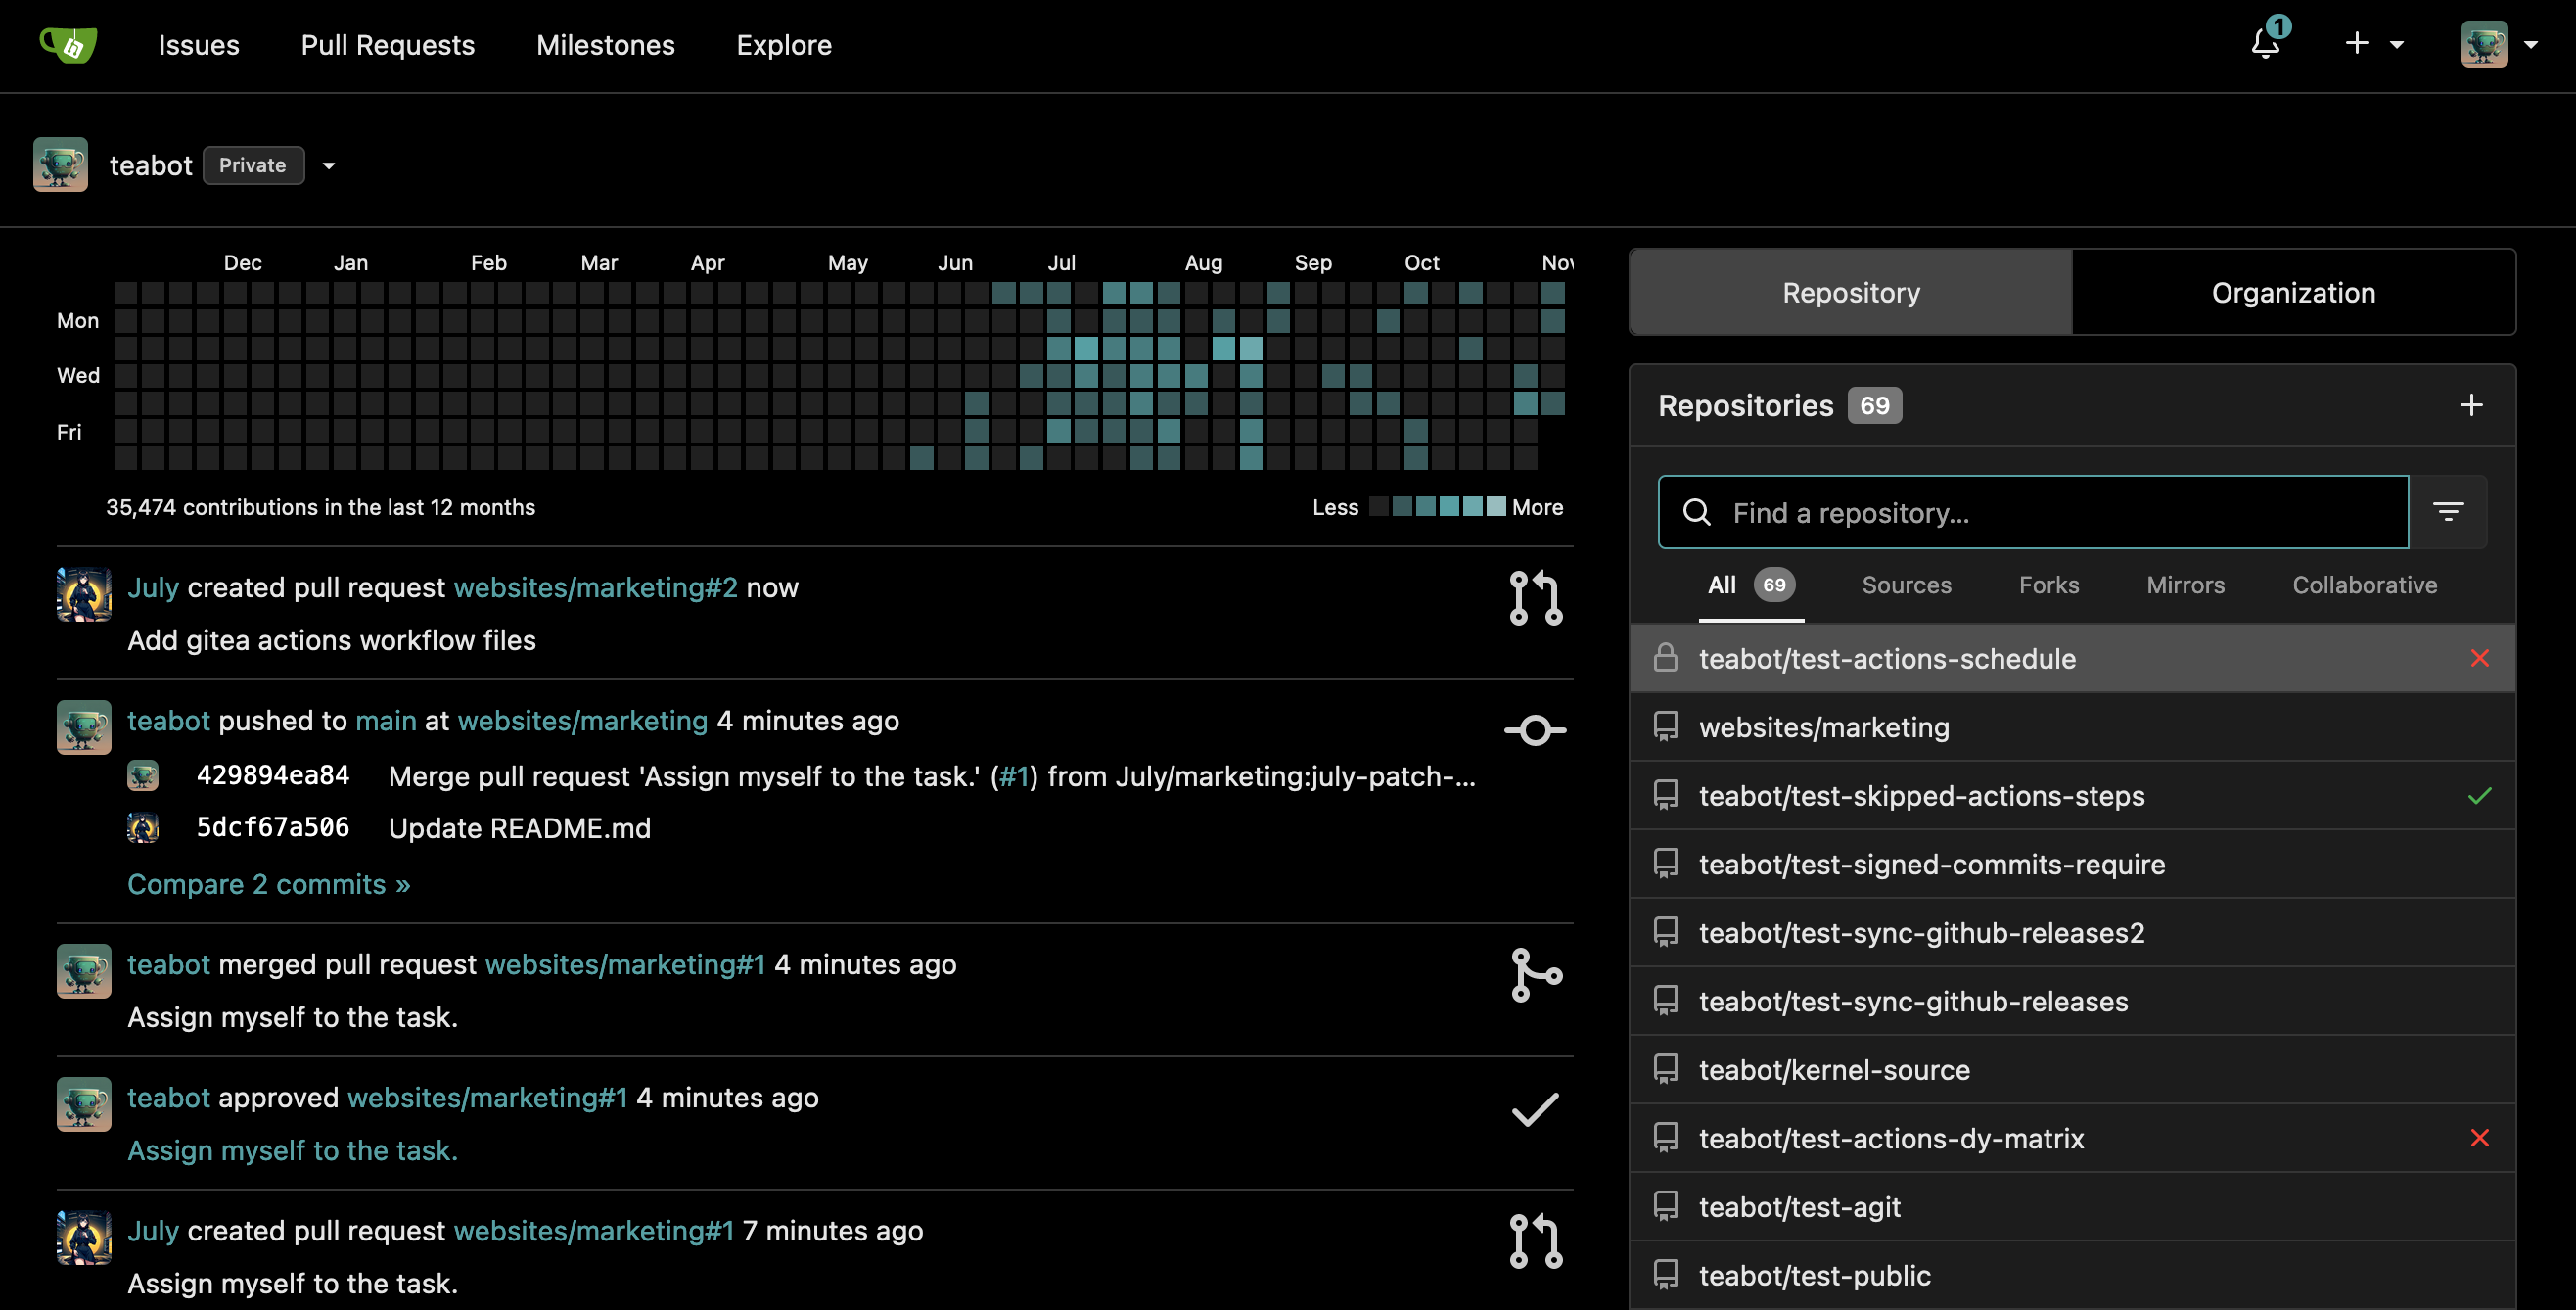
\includegraphics[width=0.9\textwidth]{imaxes/gitea-ui.png}
  \caption{Screenshot of the Gitea interface}
  \label{fig:gitea-ui}
\end{figure}

\subsection*{GitLab CE 18.0}

GitLab Community Edition (CE) is an open-source Git forge licensed under the MIT license~\cite{gitlab-docs}. It supports both self-hosted and cloud-hosted deployment. GitLab CE provides Git repository management, issue tracking, merge requests, wikis, and a native \gls{cicd} system. Additional tools include container registry support, role-based access control, and project analytics.

\subsection*{GitHub}

GitHub is a proprietary Git forge provided as a cloud-based service~\cite{github-docs}. It includes Git repository hosting, pull requests, issue tracking, integrated GitHub Actions for \gls{cicd}, project boards, and repository wikis. While a self-hosted variant exists (GitHub Enterprise), most users interact through GitHub.com.

GPUL currently uses GitHub alongside a legacy \texttt{git daemon}. The service is publicly accessible at \url{https://github.com/gpul-org}.

%--------------------------------------------------------------------
\section{Team Chat Platforms}

\textbf{Importance.} Real-time chat platforms are the central hub for informal communication and day-to-day coordination in many organizations. They foster community engagement, enable rapid problem-solving, and are invaluable for onboarding new members. For a community-driven association like GPUL, such a platform is essential for both synchronous and asynchronous interactions. Adopting a self-hosted solution would also provide full data ownership and control over the primary communication tool, aligning with the association's core values.

\subsection*{Current stack}

GPUL currently uses a mix of Telegram and Discord for day-to-day communication. While both are widely adopted and convenient, they are externally managed proprietary platforms. This limits flexibility, ownership, and long-term sustainability of the communication infrastructure.

\subsection*{Matrix (Element)}

Matrix is an open standard protocol for real-time communication, supporting decentralization and end-to-end encryption. It operates through independently hosted \emph{homeservers}, which synchronize using federation. The most widely used homeserver implementation is \texttt{Synapse}, written in Python. The reference client, \texttt{Element}, provides a web-based interface with features such as threads, rooms, voice/video calls, and file sharing. Federation and bridging to other platforms (e.g., IRC, Slack, Discord) are natively supported. Matrix is licensed under the Apache License 2.0~\cite{matrix-docs}. A screenshot of the Element interface is shown in Figure~\ref{fig:element-ui}.

\begin{figure}[h!]
  \centering
  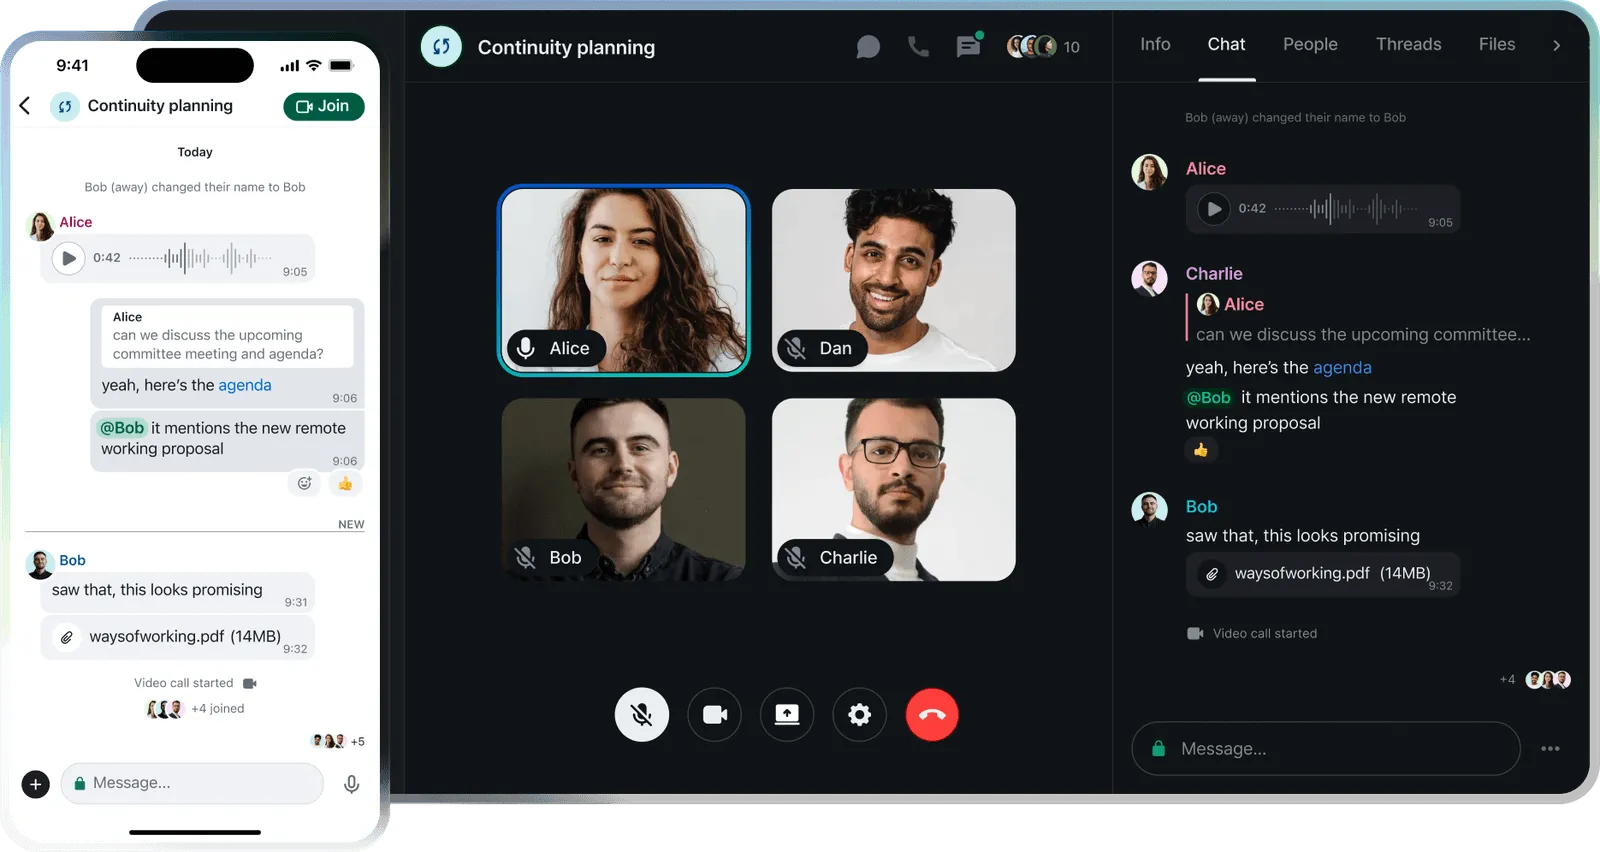
\includegraphics[width=0.9\textwidth]{imaxes/element-ui.png}
  \caption{Screenshot of the Element chat interface}
  \label{fig:element-ui}
\end{figure}

\subsection*{Mattermost}

Mattermost is a self-hosted team messaging platform released under the MIT License~\cite{mattermost-docs}. It provides channel-based discussions, searchable history, file attachments, and integrations through slash commands, bots, and plugins. The architecture is monolithic and typically deployed with a PostgreSQL backend. Mattermost supports SSO, LDAP, and OAuth2 authentication, and offers a web interface, desktop, and mobile clients. A screenshot of the Mattermost interface is shown in Figure~\ref{fig:mattermost-ui}.

\begin{figure}[h!]
  \centering
  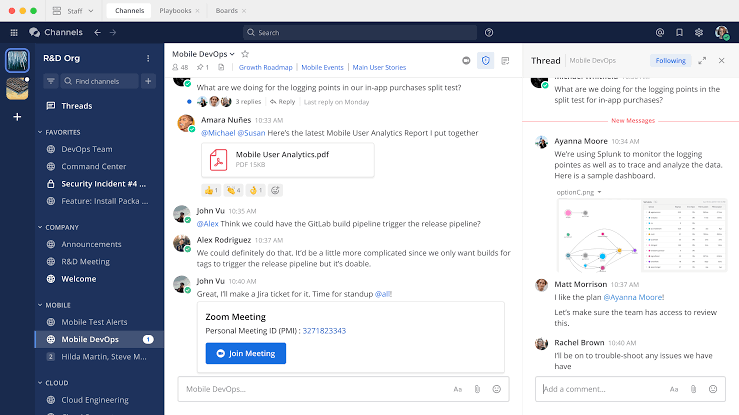
\includegraphics[width=0.9\textwidth]{imaxes/mattermost-ui.png}
  \caption{Screenshot of the Mattermost chat interface}
  \label{fig:mattermost-ui}
\end{figure}

\subsection*{Nextcloud Talk (Chat)}

Nextcloud Talk includes a chat component within the broader Nextcloud groupware ecosystem. It allows persistent one-to-one and group conversations with notifications and shared file integration. The code is licensed under AGPLv3~\cite{nextcloud-talk-docs}.

\subsection*{Proprietary Alternatives}

Closed-source platforms like Discord, Slack, and Telegram offer feature-rich environments but rely on external servers and proprietary ecosystems. These tools are not further considered due to the lack of data sovereignty and alignment with the association's open-source values.

%--------------------------------------------------------------------
\section{Secrets / Password Vault}

\textbf{Importance.} Securely managing shared credentials is a fundamental security requirement for any organization. Password vaults provide encrypted storage, role-based access control, and auditability, mitigating the significant risks associated with ad-hoc methods like sharing plaintext files. This is a critical need for GPUL, whose current practices are insecure. Implementing a dedicated vault is essential to protect the association's infrastructure, services, and member data.

\subsection*{Current stack}
GPUL currently stores shared passwords in a plaintext file within the Nextcloud instance. This solution lacks encryption, granular access control, and audit trails.

\subsection*{Bitwarden Server}
Bitwarden is a password manager licensed under AGPLv3 with both a self-hosted server and an official cloud offering. It supports client-side AES-256 encryption, role-based access control, and sharing via collections and groups. Vaults are stored in a PostgreSQL database with encrypted attachments. Comprehensive documentation is available online~\cite{bitwarden-docs}.

\begin{figure}[h!]
  \centering
  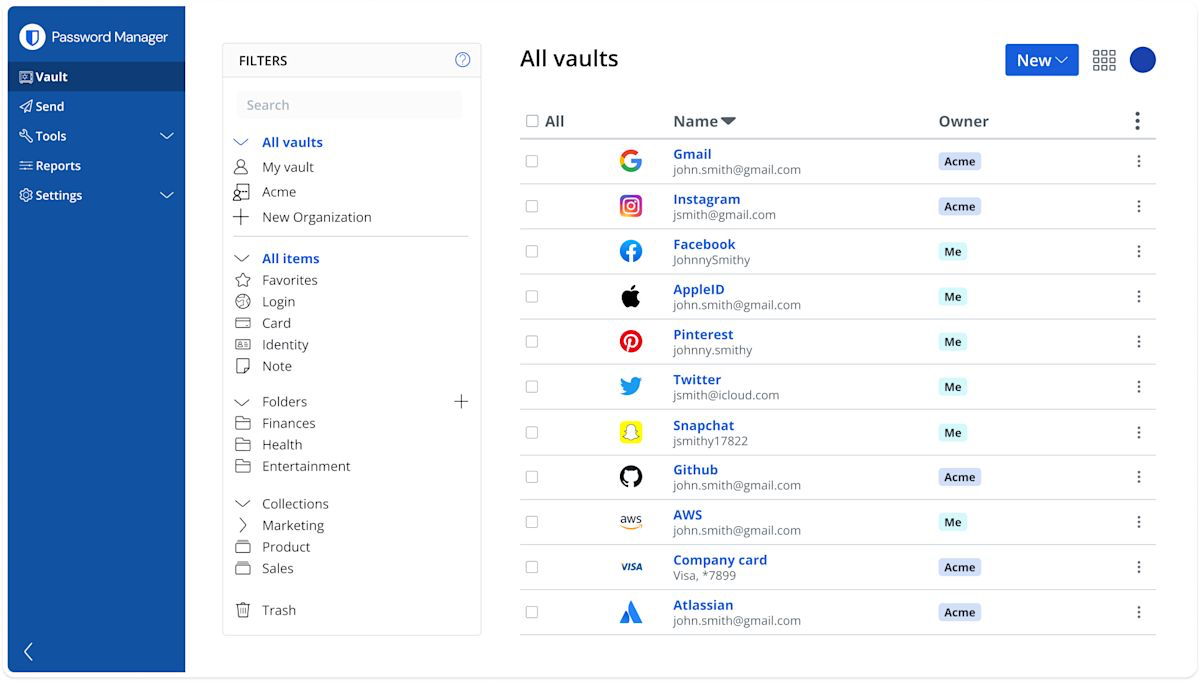
\includegraphics[width=0.9\textwidth]{imaxes/bitwarden-ui.png}
  \caption{Screenshot of the Bitwarden password manager interface}
  \label{fig:bitwarden-ui}
\end{figure}

\subsection*{Passbolt 4}
Passbolt is a web-based team password manager licensed under AGPLv3~\cite{passbolt-security}. It uses OpenPGP encryption in the browser, with each password encrypted for specific users' keys. It supports fine-grained sharing, activity logs, and uses a MySQL-compatible backend. Unlike Bitwarden, it requires users to manage their private \gls{gpg} keys.

\subsection*{HashiCorp Vault 1.17}
Vault is a general-purpose secrets manager aimed at infrastructure-level secrets rather than password sharing. It supports dynamic secrets, time-to-live (TTL) credentials, and multiple authentication backends (e.g., GitHub, LDAP). Secrets are encrypted server-side and stored in a pluggable backend such as files, Consul, or PostgreSQL. Vault is source-available under the BSL 1.1 license~\cite{vault-bsl}.

\subsection*{Proprietary Alternatives}
Popular proprietary services like 1Password, LastPass, and Keeper offer similar functionality but require the use of externally hosted infrastructure. Due to GPUL's preference for open-source and self-hosted tools, these are excluded from further evaluation.

%--------------------------------------------------------------------
\section{Monitoring \& Logging}

\textbf{Importance.} Monitoring and logging are essential for ensuring the stability and performance of critical services, providing visibility into system behavior to help administrators detect and resolve issues proactively. For a volunteer-run, community-managed infrastructure like GPUL's, it is crucial for preventing service degradation, reducing downtime, and easing the burden on future maintainers.

\subsection*{Current stack}
Currently, no formal monitoring stack is in place. Most services log to local files with no rotation configured, often resulting in uncontrolled disk usage. There is no log centralization, alerting, or metric tracking, making it difficult to respond proactively to incidents.

\subsection*{Prometheus + Grafana + Loki}
A popular open source stack for monitoring and logging is the combination of Prometheus, Grafana, and Loki. Prometheus is a time-series database and alerting system that collects numeric metrics from instrumented services via HTTP endpoints~\cite{prometheus-docs}. It supports service discovery, pull-based scraping, and label-based queries using PromQL. Grafana acts as a dashboard and visualization layer, connecting to Prometheus and other sources to present interactive panels, graphs, and alerts. Loki is a log aggregation system inspired by Prometheus: it stores log streams with associated labels, allowing queries using LogQL~\cite{loki-docs}. Unlike traditional log engines, Loki only indexes metadata, making it efficient and lightweight.

Each component is open source: Prometheus is under the Apache 2.0 license, while Grafana and Loki are licensed under AGPLv3~\cite{grafana-license-change}. Together, they form a well-integrated observability suite, often referred to as the PLG stack.

\subsection*{Zabbix}
Zabbix is a mature open source monitoring solution that uses a central server and lightweight agents~\cite{zabbix-web}. It supports metric collection through agents, SNMP, IPMI, and scriptable checks. Zabbix provides a web interface for dashboards and alerts, and includes automatic discovery, distributed proxies, and a large template library. It stores metrics in SQL databases and is licensed under AGPLv3. A screenshot of the interface is shown in Figure~\ref{fig:zabbix-ui}.

\begin{figure}[h!]
  \centering
  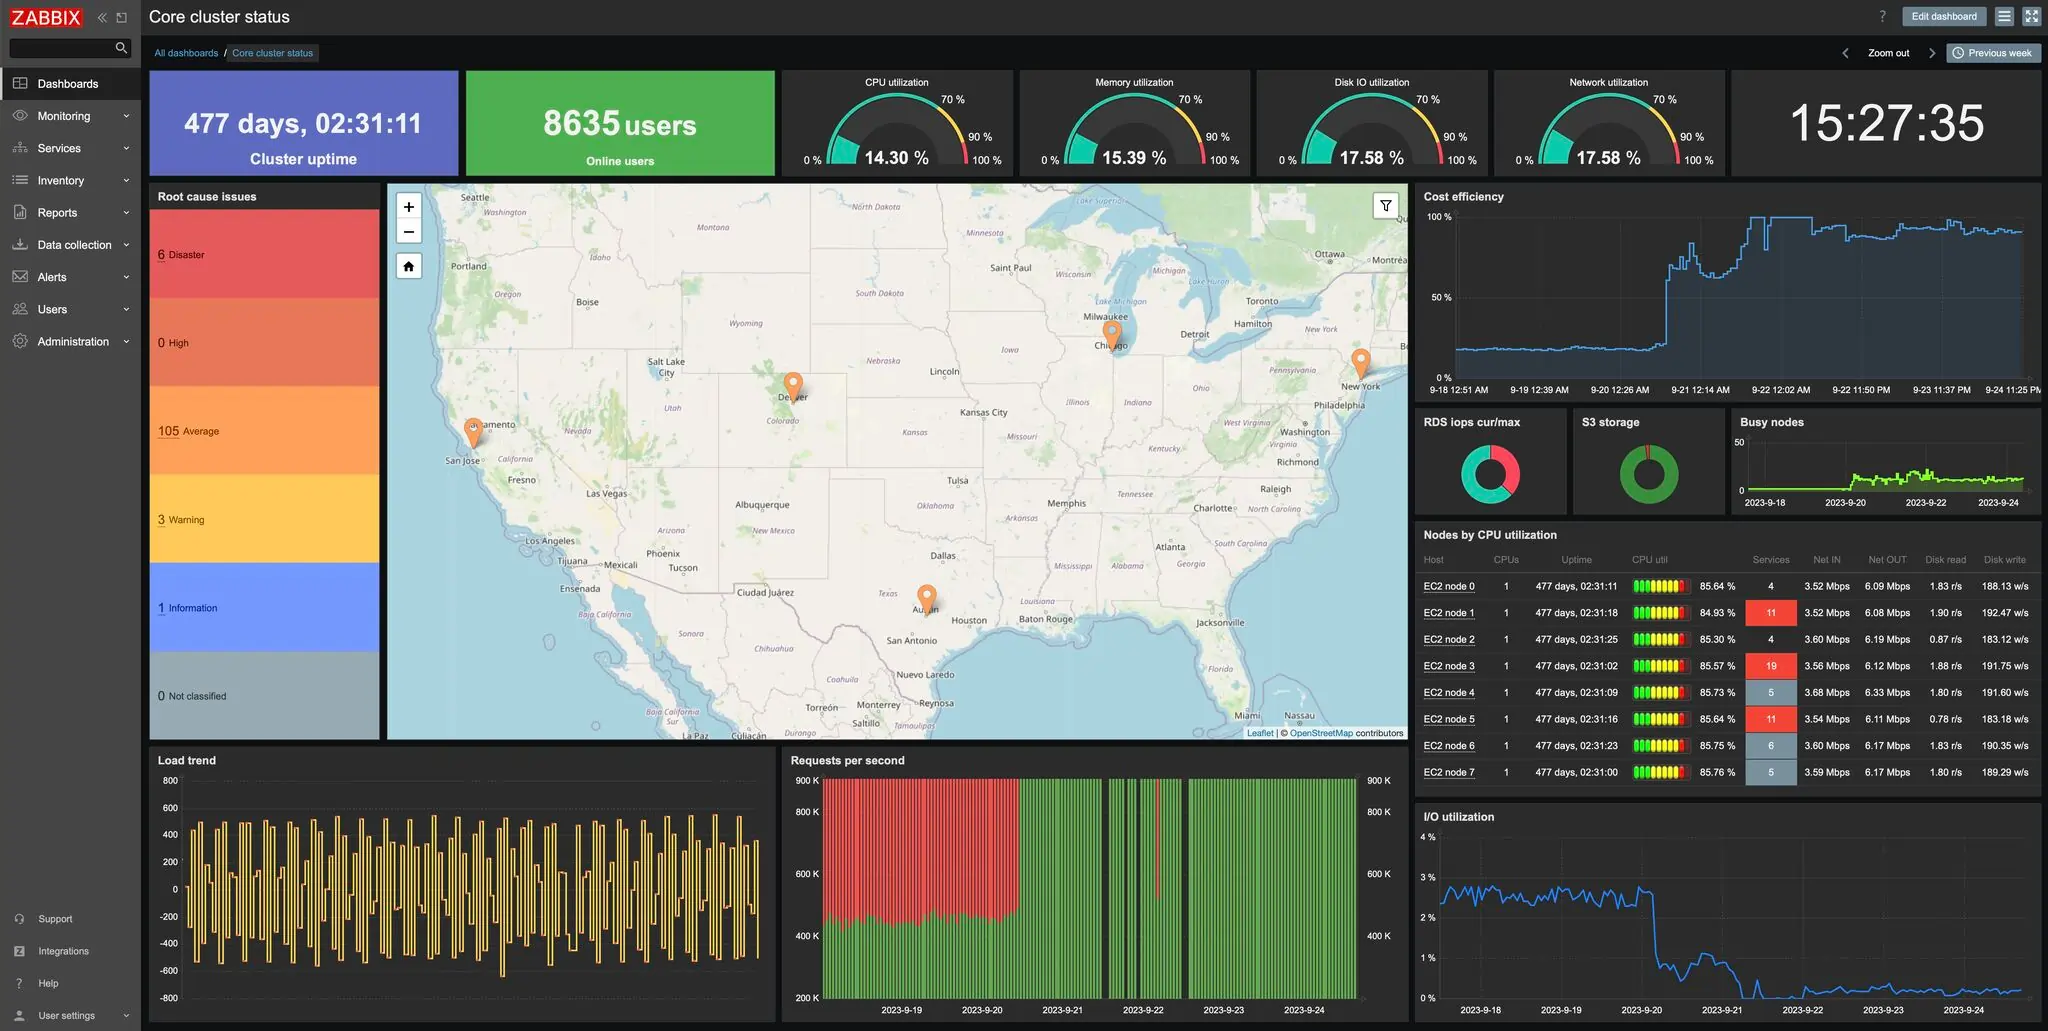
\includegraphics[width=0.9\textwidth]{imaxes/zabbix-ui.png}
  \caption{Screenshot of the Zabbix monitoring dashboard}
  \label{fig:zabbix-ui}
\end{figure}

\subsection*{OpenSearch Dashboards (formerly ELK)}
The ELK stack—Elasticsearch, Logstash, and Kibana—is widely used for log aggregation and analysis. Elasticsearch handles indexing and querying, Logstash parses and ships logs, and Kibana provides visualization. The original ELK stack shifted away from open source licenses, but forks like OpenSearch continue under Apache 2.0~\cite{opensearch-web}. Alternatively, Elastic recently reintroduced AGPLv3 licensing for their stack~\cite{elastic-license}. While powerful, the ELK/OpenSearch stack is resource-intensive and typically more complex to manage.

\subsection*{Proprietary Alternatives}
Cloud-based observability platforms such as Datadog, New Relic, and Splunk offer complete solutions with minimal setup and powerful features. However, their pricing models, data sovereignty implications, and closed-source nature make them less suitable for GPUL's goals of open, self-hosted, and cost-effective infrastructure~\cite{datadog-web}.

%--------------------------------------------------------------------
\section{Event Ticketing \& CFP Tooling}

\textbf{Importance.} For many associations, events are a core activity requiring tools for ticketing, registration, and speaker management. An integrated platform can streamline these workflows, reduce administrative overhead, and improve the experience for organizers and attendees. Events are a fundamental part of GPUL's community outreach, but the current reliance on separate proprietary services introduces friction and cost. Adopting a unified, self-hosted tool would align with the association's values while providing greater control and a more professional appearance.

\subsection*{Current stack}
GPUL currently uses a mix of proprietary platforms. \emph{Meetup} is used to promote and coordinate free, recurring meetups. For larger events requiring registration and payment, \emph{Eventbrite} is employed. For call-for-proposals (CFPs), the hosted service \emph{pretalx.com} has been used.

\subsection*{pretalx}
\textbf{pretalx} is an open-source system for managing the full CFP process: submission, review, scheduling and communication. It allows custom submission forms, anonymous or public review workflows, and includes a schedule editor with conflict detection and speaker availability~\cite{pretalx-docs}. The software is written in Python (Django), supports plugins, and is licensed under Apache~2.0~\cite{pretalx-license}. A hosted service is also available for events that prefer not to self-host. A screenshot of the interface is shown in Figure~\ref{fig:pretalx-ui}.

\begin{figure}[h!]
  \centering
  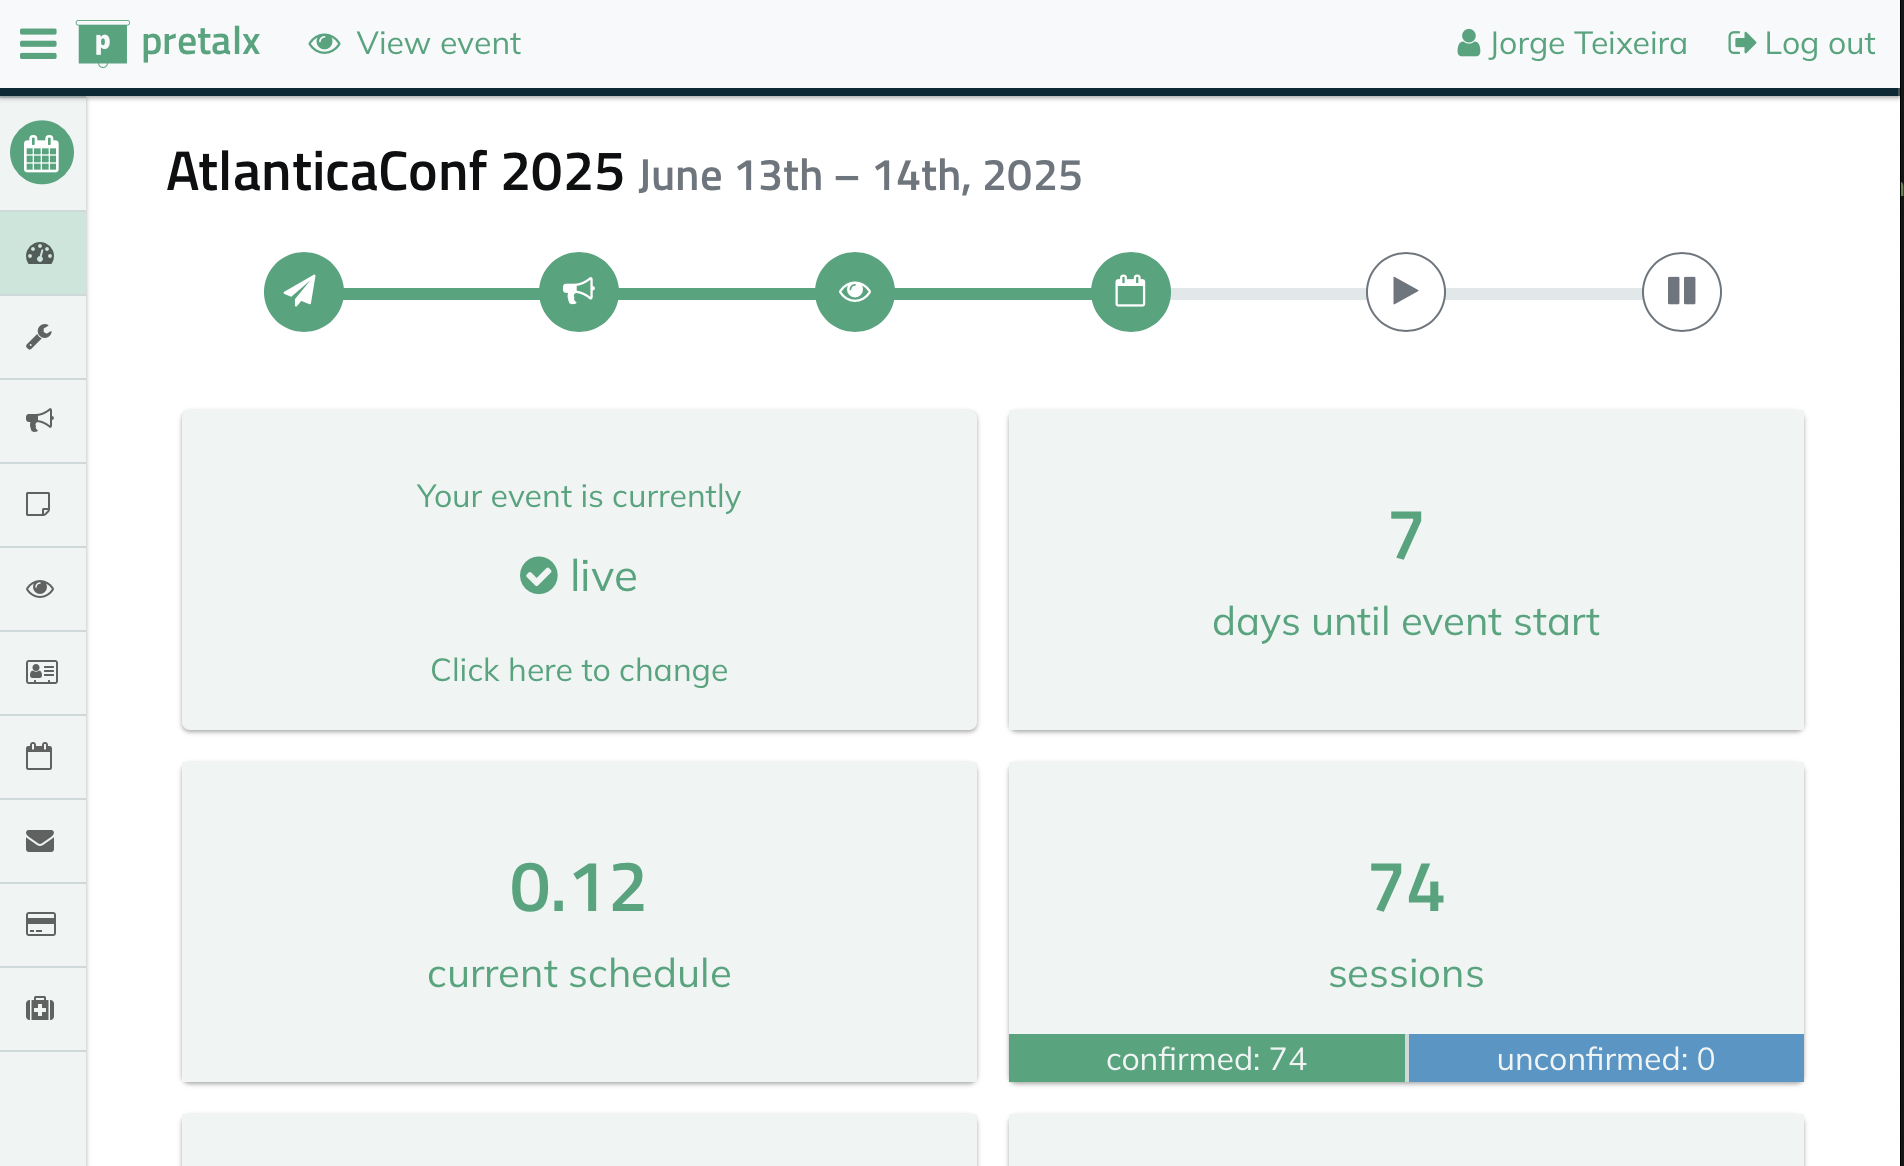
\includegraphics[width=0.9\textwidth]{imaxes/pretalx.com-ui.png}
  \caption{Screenshot of the pretalx conference management interface}
  \label{fig:pretalx-ui}
\end{figure}

\subsection*{pretix}
\textbf{pretix} is a feature-rich ticketing platform for events. It provides a configurable online shop, generates e-tickets, supports multiple payment gateways, and includes mobile apps for check-in~\cite{pretix-docs}. It is released under the AGPLv3 license and supports plugins for extensibility.

\subsection*{Koliseo}
\textbf{Koliseo} is an integrated open-source platform covering CFP, scheduling, and ticketing. It includes submission and agenda tools as well as QR-based ticketing using Stripe for payments. It is released under the Apache~2.0 license and offers a hosted version with a freemium model~\cite{koliseo-website}.

\subsection*{Indico}
\textbf{Indico}, developed at CERN, is a comprehensive event platform supporting abstracts, reviews, scheduling, registration, and badge printing. It is designed to scale and includes academic-focused features such as paper submissions and room booking~\cite{indico-github}. It is written in Python (Flask) and released under the MIT license.

\subsection*{Proprietary Alternatives}
While this report focuses on open-source alternatives, GPUL currently relies on several proprietary services:

\begin{itemize}
  \item \textbf{Meetup}: Useful for visibility and community-building but limited in custom workflows. Organizers must pay a yearly subscription of around 200 €~\cite{meetup-wiki}.
  \item \textbf{Eventbrite}: Used for ticketing paid events. Charges a fee of around 10\% per ticket and does not support CFP~\cite{eventbrite-wiki}.
  \item \textbf{pretalx.com}: Hosted version of the open-source pretalx tool. Charges per event~\cite{pretalx-pricing}.
\end{itemize}

%--------------------------------------------------------------------
\section{Invoicing / Accounting}

\textbf{Importance.} Compliant invoicing and accounting are a legal necessity for any formally constituted association, governed by national and regional regulations. This is a particularly pressing issue in Spain, where upcoming \textbf{VeriFactu} regulations will mandate certified electronic invoicing systems that report to the tax agency (AEAT) in real-time. For GPUL, abandoning manual, non-compliant methods is not merely an upgrade but a mandatory step to ensure legal and fiscal viability \cite{odoo-blog-verifactu}.

\subsection*{Current stack}
LibreOffice templates stored in Nextcloud, with manual PDF generation and signing. No Facturae, XML or AEAT compliance is currently met. A screenshot of the current invoice template is shown in Figure~\ref{fig:invoice}.

\begin{figure}[h!]
  \centering
  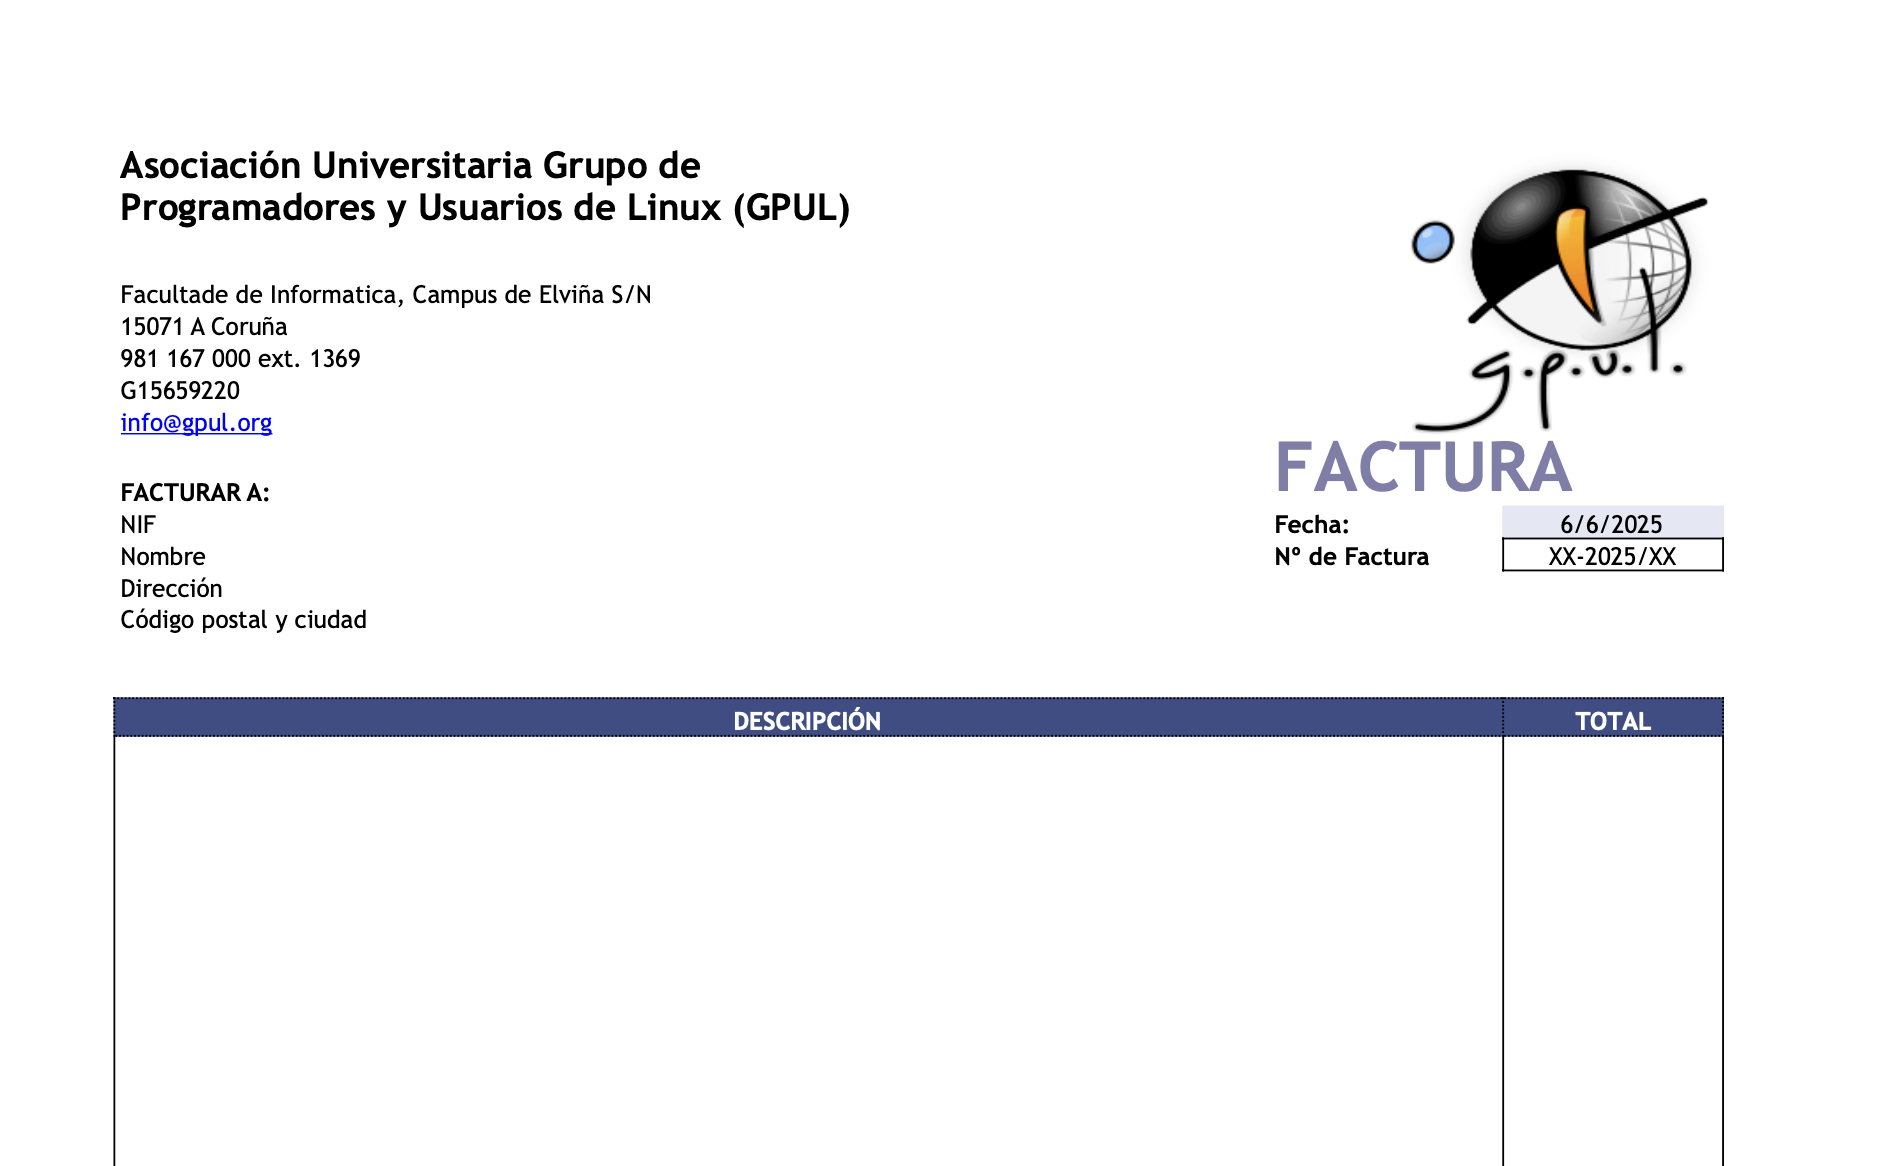
\includegraphics[width=0.9\textwidth]{imaxes/invoice.png}
  \caption{Example of the invoice template currently used}
  \label{fig:invoice}
\end{figure}

\subsection*{Odoo}
Full \gls{erp} with accounting and invoicing modules. Spanish localization modules allow Facturae XML export, AEAT integration, SII support and planned VeriFactu readiness \cite{odoo-einvoice-spain}. Heavy stack and learning curve, but suitable for full integration. A screenshot of the interface is shown in Figure~\ref{fig:odoo-ui}.

\begin{figure}[h!]
  \centering
  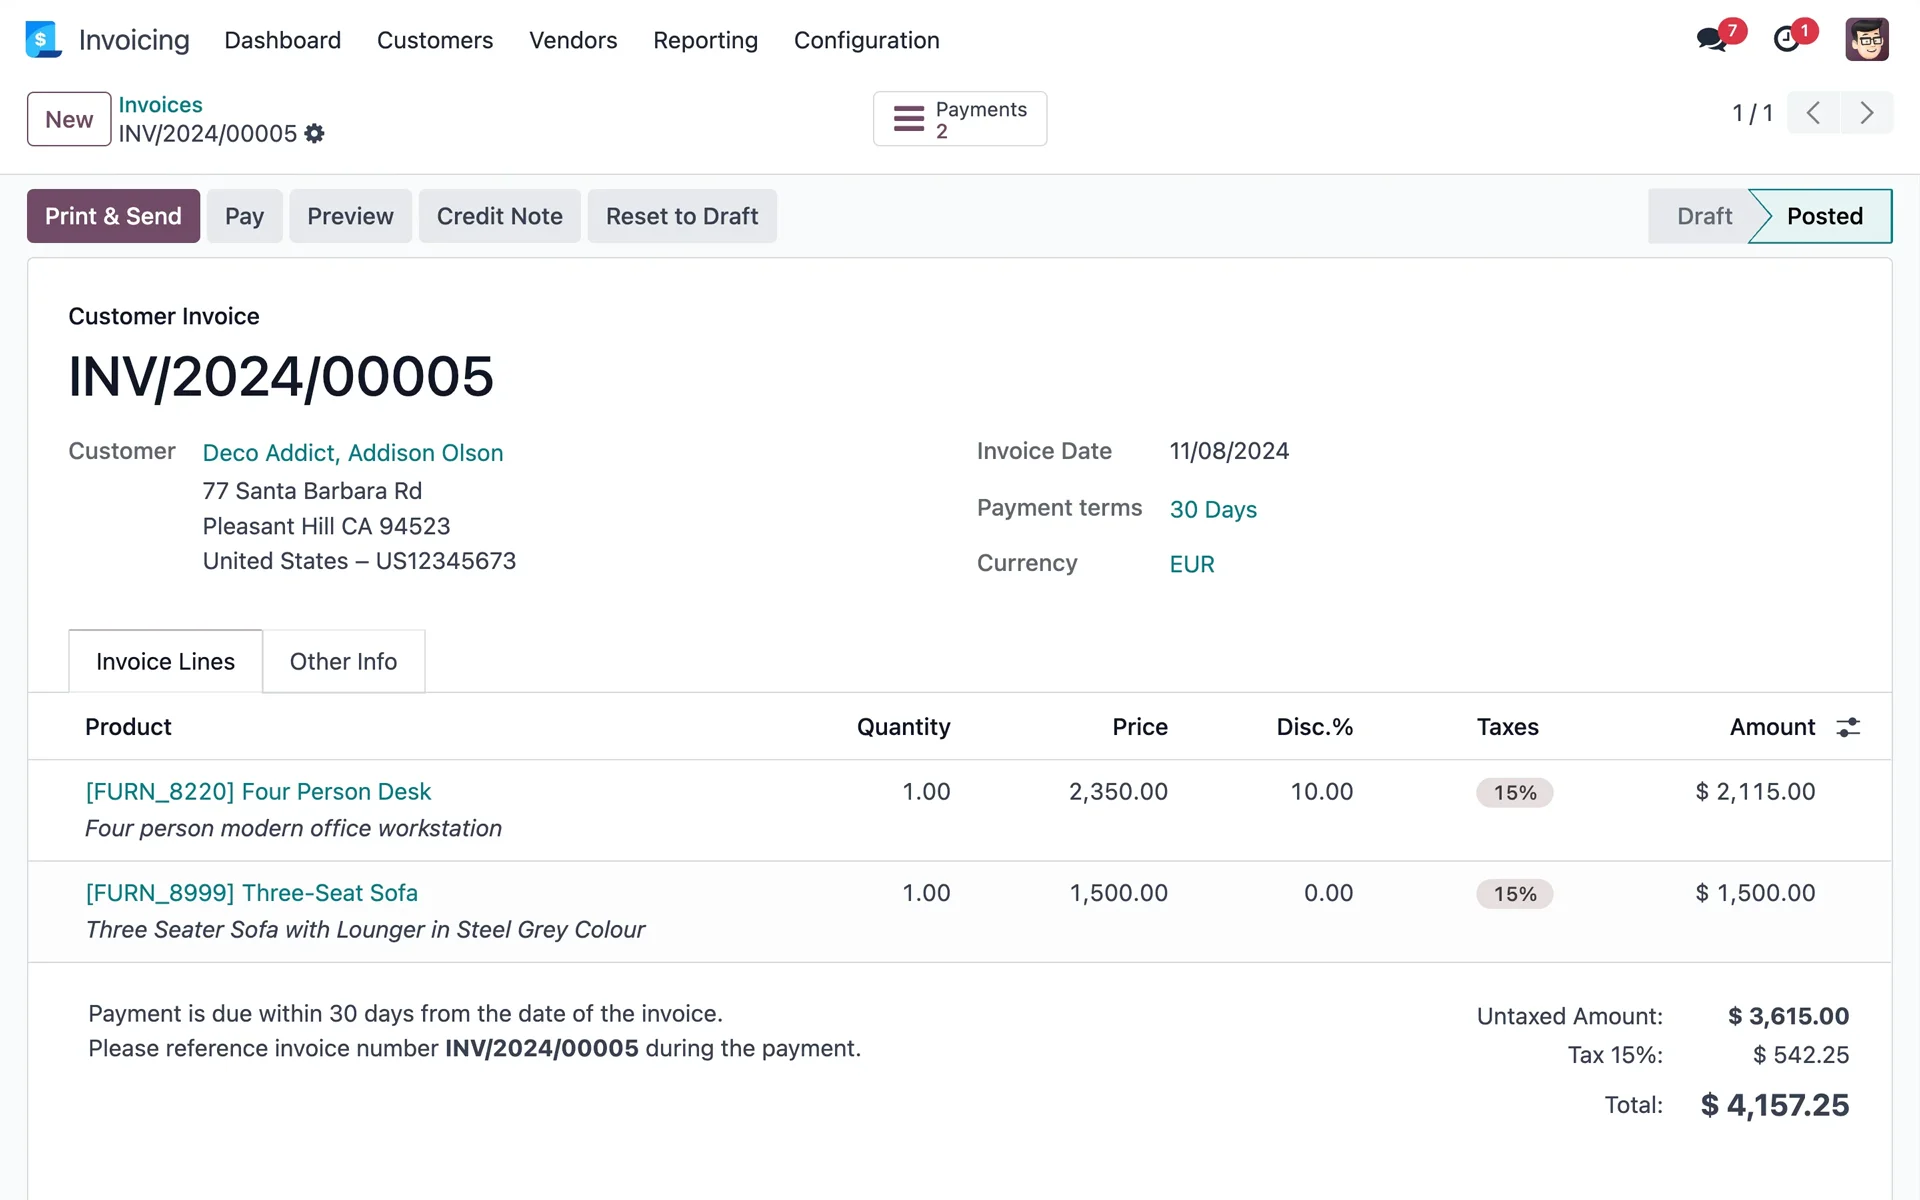
\includegraphics[width=0.9\textwidth]{imaxes/odoo-ui.png}
  \caption{Screenshot of the Odoo management interface}
  \label{fig:odoo-ui}
\end{figure}

\subsection*{FacturaScripts}
Spanish-made open source \gls{erp} with strong native support for Facturae and IRPF/IVA reporting. Plugin system allows automatic signing and XML export \cite{facturascripts-antifraude}. VeriFactu modules are planned by the maintainers.

\subsection*{Proprietary Alternatives}

\textbf{Holded} and \textbf{Quipu} are both popular Spanish cloud ERPs with direct AEAT and VeriFactu compliance out of the box \cite{holded-verifactu}. \textbf{Sage} offers several solutions (Sage 50, Sage Despachos) and promotes VeriFactu-compliant accountant platforms \cite{sage-verifactu}.

\subsection*{External Accountant}
A viable route is outsourcing invoice issuance and reporting through a accounting firm. Most use certified tools (e.g., Sage) and provide invoice portals. This model outsources technical complexity and ensures compliance, but implies higher cost and less internal control \cite{sage-blog-asesoria}.

%--------------------------------------------------------------------
\section{Service Deployment and Management}

\textbf{Importance.} A reliable and reproducible deployment workflow is crucial for the long-term sustainability of any technical infrastructure, especially one managed by volunteers. It ensures that services can be easily replicated, recovered from failures, and maintained by future members. For GPUL, the current mix of bare-metal and manual container deployments is fragile and poorly documented. Adopting a modern virtualization or orchestration platform is essential to create a resilient, scalable, and manageable infrastructure for the future.

\subsection*{Current stack}
The current infrastructure consists of a mixture of services deployed directly on bare metal and others managed via \texttt{docker-compose}, spread across two physical servers. There is no centralized management layer, which complicates monitoring, scaling, and service replication. Containers are started manually, with limited documentation or automation.

\subsection*{Proxmox VE}

Proxmox Virtual Environment (VE) is an open-source virtualization management platform (Debian-based) that integrates KVM-based virtual machines and LXC containers \cite{proxmox-admin-guide-2025}. It provides a unified web-based interface and \gls{cli} for creating and managing VMs and containers, aiming for ease of administration so that even novices can deploy it within minutes. Proxmox can run on a single server or in a multi-node cluster (with a multi-master design and a clustered filesystem) to enable high availability and live migration of workloads. It supports flexible storage backends (local or shared storage) and includes a fully integrated backup/restore solution (via Proxmox Backup Server or vzdump) for protecting VM and container data. These features make Proxmox suitable for self-hosted labs needing a mix of VM and container workloads managed in a unified open-source platform. A screenshot of the interface is shown in Figure~\ref{fig:proxmox-ui}.

\begin{figure}[h!]
  \centering
  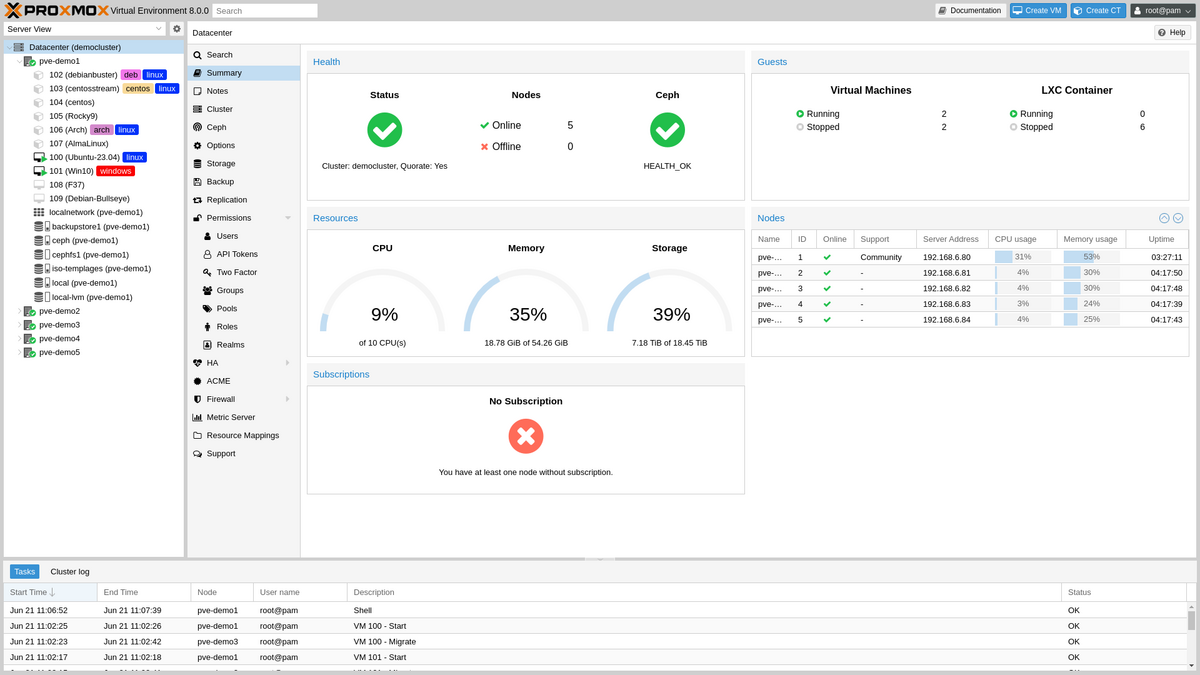
\includegraphics[width=0.9\textwidth]{imaxes/proxmox-ui.png}
  \caption{Screenshot of the Proxmox management interface}
  \label{fig:proxmox-ui}
\end{figure}

\subsection*{Incus (LXD)}

Incus is a modern open-source container and VM manager (a fork of LXD) that provides a cloud-like experience on Linux hosts \cite{incus-linux-containers-2023}. It is image-based and supports a wide range of Linux distributions, providing both system containers (sharing the host kernel) and application containers, as well as full virtual machines with guest kernels. Incus uses a single command-line tool and \gls{restapi} for local or remote management of instances, with features like snapshots, live migration, and resource profiling. It is designed to scale from a single node up to large clusters (thousands of servers)  and works on any recent Linux distribution (packages available via various distros). In practice, Incus is used for lightweight virtualization on commodity hardware, where administrators want to mix containers and VMs with relatively low overhead and a straightforward \gls{cli}/API interface.

\subsection*{Docker and Podman}

Docker and Podman are containerization platforms for running applications in isolated environments. Docker (Docker Engine) popularized this approach by packaging code and dependencies into portable containers \cite{spacelift-podman-docker-2024}. It follows a daemon-based model and supports layered images and declarative Dockerfiles. Docker also provides Docker Compose for defining multi-container applications via a single YAML file and a Swarm mode for basic clustering and service replication. Podman is a daemonless, rootless container engine (a drop-in Docker replacement) that runs containers as child processes of the user, improving security isolation. Podman supports most Docker \gls{cli} commands and introduces "pods" (groups of containers sharing the same network namespace) similar to Kubernetes pods. For orchestration, Docker relies on Docker Compose and Swarm, whereas Podman can use \texttt{podman-compose} or generate Kubernetes manifests; Podman itself has no built-in high-availability orchestrator. Podman is often favored in security-sensitive or multi-user environments (and is default on many Linux distributions), while Docker remains widely used in development and CI/CD environments due to its mature ecosystem and tools.

\subsection*{Kubernetes}

Kubernetes is an open-source container orchestration system originally developed by Google \cite{kubernetes-docs-2025}. It automates deployment, scaling, and management of containerized applications. Kubernetes groups containers into logical units called \emph{pods} (each pod contains one or more containers with shared storage and networking). A Kubernetes cluster typically includes a control-plane (master) and multiple worker nodes; users define desired application state via declarative manifests (Deployments, Services, etc.), and Kubernetes automatically schedules pods onto nodes. The platform handles service discovery, load balancing, rolling updates/rollbacks, and self-healing (restarting failed containers). It "provides a framework to run distributed systems resiliently," automatically handling scaling, failover, and automated rollouts. Kubernetes also supports secrets/config management and horizontal pod autoscaling. However, Kubernetes has substantial operational complexity and resource requirements. For small-scale setups, lightweight distributions like k3s or MicroK8s strip out legacy components to simplify installation and reduce footprint, making Kubernetes feasible even for edge or two-node deployments \cite{k3s-microk8s-2022}. In summary, Kubernetes excels in orchestrating multi-host container clusters with advanced features, whereas simpler tools (like Docker Compose or single-node Incus/Proxmox) may suffice for smaller self-hosted environments.

\subsection*{Proprietary Alternatives}

There are several proprietary platforms offering infrastructure orchestration and service management, such as VMware vSphere, Red Hat OpenShift, and Amazon ECS. However, in this particular domain, open-source solutions are not only mature and widely adopted, but also provide superior flexibility, transparency, and long-term maintainability. As such, proprietary tools are not considered viable contenders for the association's use case.

  % SPDX-FileCopyrightText: 2025 Jorge Teixeira Crespo <jorge.teixeira@udc.es>
%
% SPDX-License-Identifier: GPL-2.0-or-later

\chapter{Technology Selection}
\label{chap:technology-selection}

\lettrine{B}{ased} on the comparative analysis in the previous chapter, this section outlines the final decisions taken for each service in the infrastructure.  
Each subsection details the chosen solution, the motivation behind the decision, and the key trade-offs considered.  
As stated previously, the focus is on ensuring coherence with GPUL's values, long-term maintainability, and the practical constraints of a volunteer-run environment.

%--------------------------------------------------------------------
\section{Mailing-list Managers}

To modernize the mailing list service while ensuring archival continuity, the project will adopt Mailman 3, alongside the HyperKitty web archiver. The primary driver for this decision is ensuring continuity with the existing Mailman 2 deployment while significantly modernizing the service. Migrating to a different platform, such as Sympa, would jeopardize the integrity and accessibility of the historical archives, which are a critical resource for the association. In contrast, Mailman 3 offers a direct and well-documented upgrade path. The migration process is highly automated, with official tools like \texttt{mailman import21} for list configuration and \texttt{hyperkitty\_import} for archives, minimizing the risk of data loss and reducing the manual effort required~\cite{mailman-migration-docs}.

Beyond the seamless migration, Mailman 3's redesigned architecture presents a significant leap forward in terms of maintainability and features. The system is now modular, with a central \texttt{Mailman Core} handling message processing and a REST API for administration. This separation of concerns not only simplifies maintenance but also allows for flexible integration with other services. For users, the most visible improvement comes from HyperKitty, which replaces the outdated Pipermail archiver~\cite{hyperkitty-docs}. It provides a modern, searchable web interface where members can easily browse, search, and even reply to conversations directly, greatly improving the accessibility of the archives.

For list administration, the suite includes Postorius, a web-based front-end to the REST API~\cite{postorius-docs}. While optional—as all tasks can be performed via the command line—its user-friendly interface for managing lists and subscribers is a key advantage for a volunteer-run infrastructure. The platform's maturity and adoption by other large open-source projects, such as the Fedora Project, further reinforces this choice. Finally, the entire Mailman 3 suite is licensed under the GNU General Public License (GPL), which fully aligns with GPUL's commitment to using and promoting free and open-source software.

%--------------------------------------------------------------------
\section{Cloud Storage / Groupware}

For cloud storage and groupware, the project will continue to use the Nextcloud platform, upgrading the current deployment to Nextcloud Hub 10. The primary motivation for this decision is to ensure service continuity and leverage existing user familiarity. By staying within the Nextcloud ecosystem, members will not need to learn a new tool, which minimizes disruption and training overhead. The migration path is considered low-risk; a new, clean instance of Nextcloud Hub 10 will be deployed, and user data will be migrated by transferring the files directly and recreating the user accounts to ensure data integrity~\cite{nextcloud-docs}.

Furthermore, Nextcloud's status as a community-driven project licensed under the AGPL aligns with GPUL's core values, setting it apart from alternatives with a heavier enterprise focus. A key strategic advantage of this choice is the seamless integration with Nextcloud Talk, the selected video conferencing platform. This creates a unified groupware suite, providing a single, cohesive environment for file management, real-time communication, and collaboration, which simplifies the overall infrastructure and user workflow.

%--------------------------------------------------------------------
\section{Video Conferencing Platforms}

As anticipated in the previous section, video conferencing capabilities will be provided by Nextcloud Talk. This decision is primarily driven by its seamless integration into the Nextcloud Hub ecosystem, creating a single, unified platform for all of GPUL's collaborative needs. By leveraging the existing infrastructure, users can schedule meetings directly from the calendar, share documents from their cloud storage during a call, and manage conversations within the same familiar interface~\cite{nextcloud-talk-docs}.

While alternatives like Jitsi Meet or BigBlueButton offer more extensive features, they were deemed overly complex and resource-intensive for the association's requirements. GPUL's typical use case involves small-scale meetings with fewer than ten participants, for which Nextcloud Talk's capabilities are perfectly sufficient. Opting for a more heavyweight solution like BigBlueButton would impose an unnecessary strain on server resources without providing tangible benefits for day-to-day operations. Therefore, Nextcloud Talk represents the most pragmatic and efficient choice, providing robust functionality where it matters most—within a tightly integrated and resource-friendly groupware environment.

%--------------------------------------------------------------------
\section{Git Forges}

For code hosting and version control, all of GPUL's repositories will be consolidated on GitHub, leading to the decommissioning of the legacy \texttt{git daemon}. While this represents a move towards a proprietary, cloud-based service, it is a pragmatic decision driven by several factors. It provides continuity, as the platform is already in use for the association's most active projects, and it ensures operational resilience. Hosting the association's infrastructure-as-code and deployment scripts on an external, highly-available platform mitigates the critical risk of a circular dependency. If the self-hosted infrastructure were to fail, the code required to restore it would remain accessible, a crucial factor for a small, volunteer-run team.

Furthermore, GitHub is the de facto standard for open-source collaboration, meaning most potential contributors are already familiar with its workflows, lowering the barrier to entry. The platform also provides significant value through its integrated features. GitHub Actions offers a powerful CI/CD system for automating builds and deployments, while GitHub Pages allows for the effortless hosting of static websites, which is ideal for things like event landing pages~\cite{github-docs}. This strategic choice allows the team to focus its limited resources on other critical services rather than on maintaining a self-hosted forge.

%--------------------------------------------------------------------
\section{Team Chat Platforms}

To establish a sovereign, community-wide communication channel, the project will deploy a self-hosted Matrix homeserver using the Synapse implementation. The primary goal is to create a centralized communication platform for the entire GPUL community, moving away from the current reliance on proprietary services. While Nextcloud Talk can be used for focused, internal collaboration among the board and activity organizers, Matrix will serve as the open forum for all members, fostering the same vibrant, community-wide interaction that currently exists on platforms like Telegram.

Matrix's architecture is ideally suited for this role. Its support for distinct channels (rooms) with varying access levels allows for the creation of public spaces for general discussion alongside private groups for specific projects. A key feature influencing this decision is Matrix's native support for bridging, which will allow the existing, active Telegram group to be connected directly to the new server~\cite{matrix-docs}. This capability ensures a smooth and gradual transition for current members. A further advantage over platforms like Mattermost is that Matrix is an open standard, not a single product. This empowers users to select their preferred client from a diverse ecosystem, rather than being restricted to an official application. By adopting Matrix, GPUL is not only gaining a powerful communication tool but also championing a leading example of a federated, open-source standard, which aligns perfectly with the association's core mission.

%--------------------------------------------------------------------
\section{Secrets / Password Vault}

To replace the insecure plaintext password file, the project will implement Passbolt, a team-oriented password manager that aligns with GPUL's security and collaboration requirements. The decision was made after ruling out other alternatives for specific reasons. HashiCorp Vault, while powerful, was dismissed as an overly complex, enterprise-focused solution; its features, such as dynamic secret rotation, are overkill for the association's needs, and its Business Source License (BSL) does not align with the project's commitment to fully open-source software~\cite{vault-bsl}.

The primary decision came down to a comparison between Passbolt and Bitwarden. While both are excellent open-source options, they are designed with different use cases in mind. Bitwarden is primarily geared towards individual use, whereas Passbolt is built from the ground up for secure team collaboration. This is most evident in its sharing model: Passbolt allows for highly granular access control, enabling the sharing of individual passwords or specific folders with different users and teams, all while providing detailed audit logs of who accessed what, and when. This is a critical feature for managing shared credentials in a volunteer organization.

From a security standpoint, Passbolt's architecture provides a stronger model for team use. It relies on end-to-end GPG encryption, where each user has a unique private key for decryption~\cite{passbolt-security}. In contrast, systems like Bitwarden derive the encryption key from a user's master password. In a team environment, this means the effective security of a shared secret is only as strong as the weakest master password among the users it is shared with. Passbolt's model avoids this issue, ensuring a more robust and consistent security posture. For these reasons, Passbolt is the clear choice to replace the insecure plaintext password file.

%--------------------------------------------------------------------
\section{Monitoring \& Logging}

To establish comprehensive observability, the infrastructure will adopt the Prometheus, Grafana, and Loki combination, commonly known as the PLG stack. This decision prioritizes a balance of power, resource efficiency, and ease of use. While powerful, alternative stacks like ELK or OpenSearch were discarded due to their significant resource consumption and steeper learning curve, which were deemed inappropriate for a volunteer-managed infrastructure.

The final decision came down to a choice between the PLG stack and Zabbix. Both platforms are highly capable and would meet the association's technical requirements. However, the PLG stack holds a significant advantage in terms of community adoption and ecosystem vibrancy. While metrics like GitHub stars can be superficial (see Figure~\ref{fig:monitoring-stars}), the broader community sentiment and contributor data suggest that Grafana Labs fosters a significantly more community-centric development model. Projects like Grafana and Loki not only accept but actively encourage external contributions, with open governance models and a track record of fast response to community pull requests~\cite{collab-grafana}. In contrast, Zabbix development remains tightly controlled by the company, with limited avenues for non-employees to influence or contribute to the core platform~\cite{zabbix-dev-policy}.

\begin{figure}[H]
  \centering
  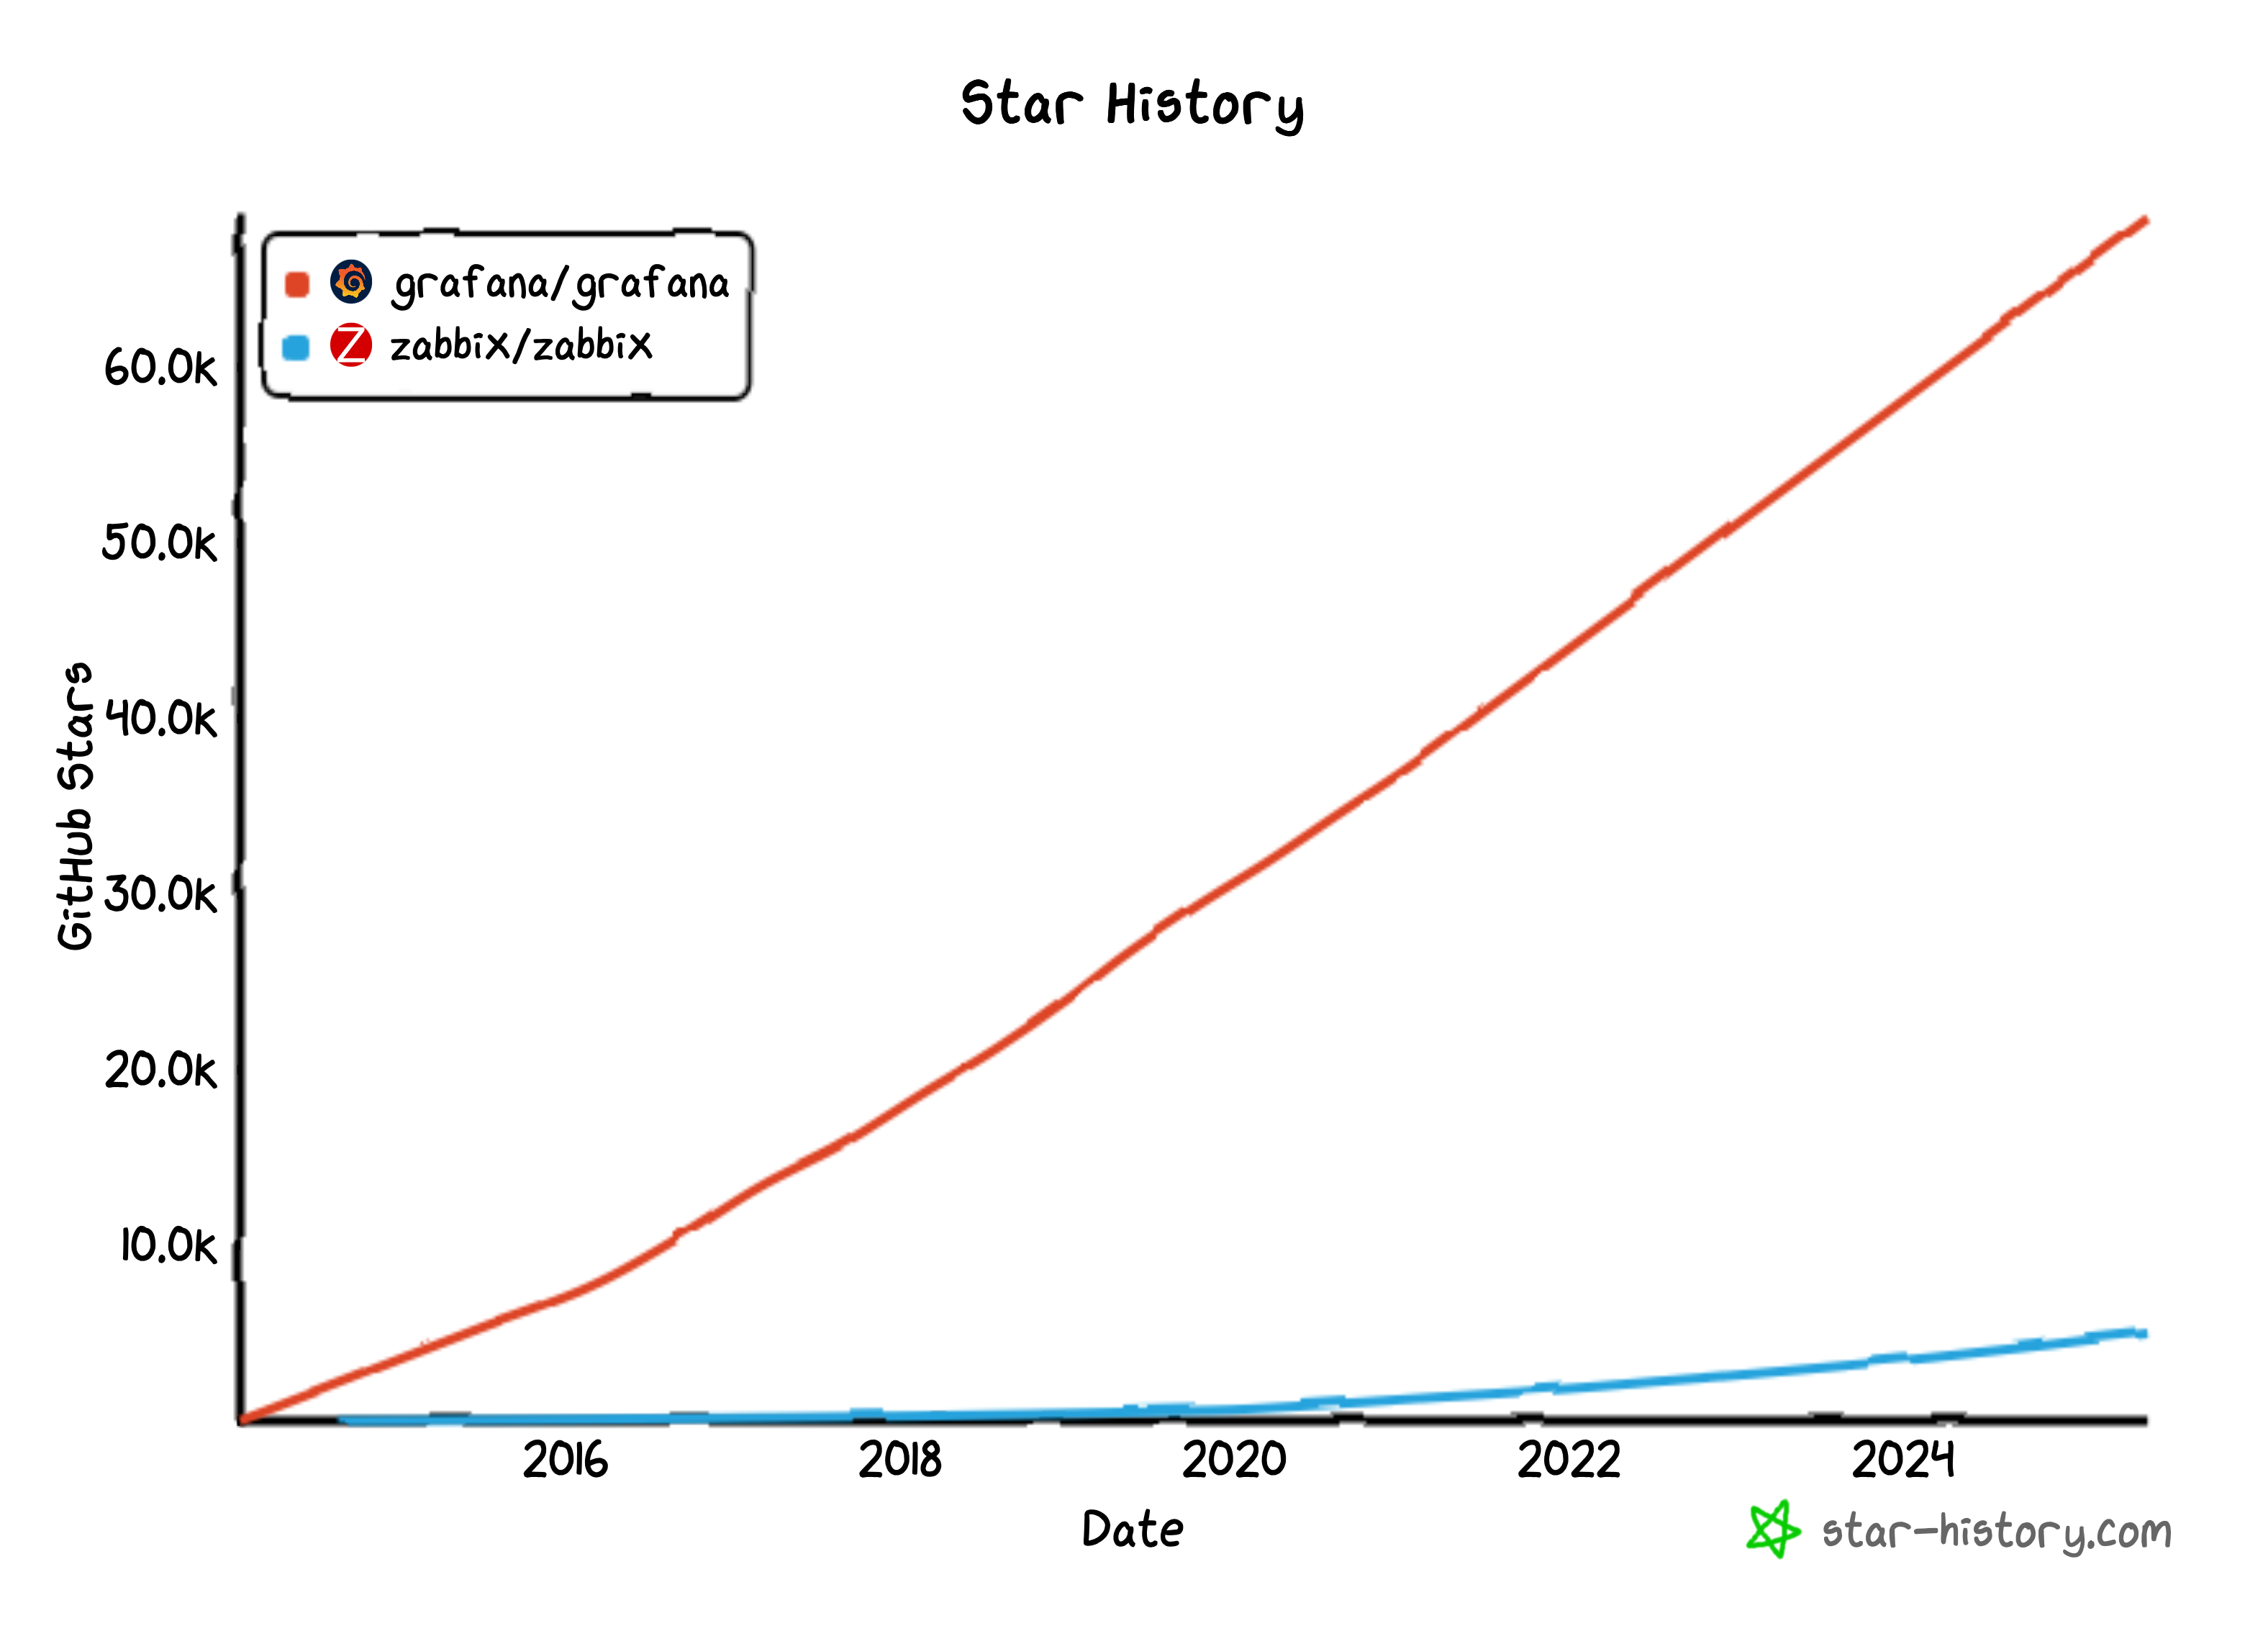
\includegraphics[width=0.9\textwidth]{imaxes/monitoring-stars.png}
  \caption{GitHub stars comparison between Grafana and Zabbix}
  \label{fig:monitoring-stars}
\end{figure}

Furthermore, the user experience and setup process heavily influenced the decision. The PLG stack is widely regarded as having a more intuitive setup and a more modern, user-friendly interface. Grafana, in particular, is renowned for its powerful and flexible visualization capabilities, making it easier to build meaningful dashboards. This view is supported by multiple online comparisons, which often highlight Grafana's superior ease of use for teams getting started with monitoring~\cite{squadcast-zabbix-grafana}. Combined with a large and responsive community, this gentle learning curve makes the PLG stack the most strategic choice for ensuring long-term maintainability in the context of a community-led infrastructure.

%--------------------------------------------------------------------
\section{Event Ticketing \& CFP Tooling}

Event management will be addressed via a phased migration, with the immediate step being the deployment of a self-hosted \textbf{pretalx} instance. This initial move is primarily driven by cost-efficiency, as it allows GPUL to stop paying for the hosted pretalx.com service while retaining the powerful call-for-proposals (CFP) and scheduling functionalities that the association already uses and values~\cite{pretalx-docs}.

For the time being, both Meetup and Eventbrite will remain in use for community outreach and paid ticketing, respectively. A full migration to a self-hosted stack is deferred due to significant non-technical considerations. Moving away from Meetup requires a careful community management strategy to avoid losing existing members and to mitigate the well-documented risk of abandoned groups being taken over by spammers, which would damage the association's reputation~\cite{combuilders-meetup-takeover}.

Similarly, replacing Eventbrite with a self-hosted alternative like pretix would necessitate integrating a third-party payment provider such as Stripe or PayPal. This carries administrative and financial responsibilities that require a formal decision from the board and is therefore considered future work. The current approach allows for an immediate cost saving while providing the time needed to address the broader strategic questions of community and financial management.

%--------------------------------------------------------------------
\section{Invoicing / Accounting}

To handle all invoicing and accounting needs, the project will implement FacturaScripts. This decision is primarily driven by the need for a solution that is both compliant with Spanish regulations and accessible to a rotating team of student volunteers. While Odoo is an extremely powerful ERP, its extensive feature set and significant learning curve were considered a disadvantage. The complexity would create a high barrier to entry for new treasurers, risking operational continuity.

FacturaScripts, in contrast, offers the ideal balance of functionality and simplicity for GPUL. As an open-source project developed in Spain, it is purpose-built to handle national fiscal requirements, including native support for Facturae and planned compliance with the upcoming VeriFactu system~\cite{FacturaScriptsAntifraude}. Its user interface is straightforward and focused on core accounting tasks, which dramatically simplifies the onboarding process for new volunteers. By providing all the necessary features without unnecessary complexity, FacturaScripts is the most sustainable choice for managing the association's finances long-term.

It is important to note that while the technical deployment of FacturaScripts will be completed as part of this project, the formal adoption for official accounting is an administrative decision reserved for the board. The final migration of financial data and processes will be carefully timed to coincide with a logical cutoff point, such as the end of a financial quarter or the start of a new fiscal year, to ensure a clean and orderly transition.

%--------------------------------------------------------------------
\section{Phone / VoIP Integration}

The university's analog phone line will be integrated into a modern VoIP system by deploying a self-hosted Asterisk server, managed via the FreePBX web interface. This combination represents the de facto standard for open-source telephony and is the only fully free and open-source alternative that meets the project's requirements~\cite{AsteriskFeatures}. Proprietary platforms like 3CX, while user-friendly, were not considered due to their licensing and cost structures.

The physical integration will be achieved using a Grandstream HT813 FXO gateway located in the GPUL office. This device will connect the analog line from the university's phone system to the Asterisk server, converting incoming and outgoing calls to SIP. To provide remote access for board members, the primary method will be deploying Grandstream HT801 Analog Telephone Adapters (ATAs) in their homes. This approach allows them to connect standard analog phones to the VoIP system, offering a reliable, physical device for making and receiving calls.

This hardware-based strategy is explicitly preferred over relying on softphone applications for mobile devices. Softphones often experience reliability issues on modern operating systems due to aggressive background process management and limited ongoing development, rendering them unsuitable for critical communications. By using dedicated ATAs, the solution ensures dependable remote access to the association's phone line for key personnel.

%--------------------------------------------------------------------
\section{Service Deployment and Management}

The underlying foundation for service deployment and management will be Incus. This decision is the result of a careful evaluation of the project's core requirements: long-term maintainability, operational simplicity for a volunteer team, and the ability to cleanly isolate services without excessive overhead. The most complex alternatives were discarded early on; Kubernetes, while powerful, is designed for multi-node orchestration and its complexity is unwarranted for a single-server deployment~\cite{KubernetesDocs2025}.

The primary contenders were Proxmox, Incus, and a bare Docker/Podman installation on a standard Linux distribution. A "bare Docker" approach was ruled out because many of the selected services are best maintained when installed directly on an operating system, following their official documentation. Forcing every service into a Docker container would often mean relying on unofficial, community-maintained images, which could complicate future maintenance. The goal is to keep each service's setup as close to the "vanilla" recommended installation as possible.

This leads to the core strategy of using system containers. Unlike application containers (like Docker), system containers (as managed by Incus) provide a full operating system userspace, sharing only the host's kernel~\cite{IncusLinuxContainers2023}. This allows each service to be installed in its own clean, isolated OS environment—for example, its own Debian container—while following the official installation guides as if it were on a dedicated machine. This approach also offers great flexibility: for services that are best deployed with Docker, a single system container can be set up with Docker installed inside it, providing a dedicated and isolated environment for running those specific application containers.

With the choice narrowed to platforms providing system containers, Incus emerged as the clear winner over Proxmox for this use case. Proxmox is an excellent, hypervisor-centric platform, but its primary advantages—a comprehensive web interface and robust virtual machine management—are not required here. The infrastructure will be managed via the command line by administrators comfortable with SSH, and there is no immediate need for full hardware virtualization. Incus provides exactly what is needed: a powerful, lightweight, and CLI-driven tool for managing system containers. As a thriving, community-led fork of LXD, it is the most efficient and versatile foundation for building a maintainable and reproducible infrastructure.

  % SPDX-FileCopyrightText: 2025 Jorge Teixeira Crespo <jorge.teixeira@udc.es>
%
% SPDX-License-Identifier: GPL-2.0-or-later

\chapter{Hosting Provider}
\label{chap:hosting-provider}

\lettrine{B}{efore} deploying any services, it was essential to choose a hosting provider that aligned with both the technical requirements of the project and the values of the association. This chapter outlines the selection process, including efforts to partner with local providers and the rationale behind the final decision.

\section{Motivations and Evaluation Criteria}

GPUL has historically prioritized working with local businesses and promoting community-centric values. In line with this, the project initially explored the possibility of deploying infrastructure on servers provided by Galician or Spanish hosting companies, ideally through a sponsorship or discount agreement. The main evaluation criteria were:

\begin{itemize}
  \item Sufficient CPU, RAM, and disk I/O performance to support containerized services
  \item Competitive and predictable pricing, ideally with sponsor support
  \item Support for IPv6 and high-bandwidth connections
  \item Root access with flexibility for custom OS installation
  \item Operational reliability and location in or near Spain
\end{itemize}

\section{Sponsorship Negotiation with a Local Provider}

One of the most promising contacts during this phase was with a Galician hosting company. After outreach and negotiation, the company offered a partial sponsorship in exchange for visibility at future GPUL events. The proposed infrastructure consisted of:

\begin{itemize}
  \item \textbf{Dedicated Server Starter (Madrid)}
    \begin{itemize}
      \item Dell PowerEdge R340
      \item Intel Xeon E-2000 (6 cores / 12 threads)
      \item 16 GB DDR4 RAM
      \item 2x240 GB SSD (boot) + 2x2 TB HDD
      \item Full management included
      \item \textit{Monthly cost after discount: €99.96 + VAT}
    \end{itemize}
  \item \textbf{VPS Cloud 5}
    \begin{itemize}
      \item 8 vCPU, 12 GB RAM, 150 GB NVMe
      \item 500 Mbps bandwidth, unmetered transfer
      \item Free of charge (fully sponsored)
    \end{itemize}
\end{itemize}

While this offer demonstrated a significant effort on the company's part to support the project, it was ultimately limited in terms of performance and flexibility, especially the low RAM on the dedicated server and the 500 Mbps cap. Furthermore, after discussions with various association members and the board, concerns were raised about the dependency that a special "discount" agreement would create with the provider.

\section{Final Decision: Hetzner Dedicated Server}

After comparing the offer from the local provider with other providers, a dedicated machine from Hetzner was selected due to its superior performance at a much lower monthly cost. The decision was also supported by the positive experiences that several members had already had with Hetzner's services. The chosen configuration was:

\begin{itemize}
  \item \textbf{Dedicated Server AX41-NVMe (Finland, HEL1)}
  \begin{itemize}
    \item AMD Ryzen 5 3600 (6 cores / 12 threads) with SMT
    \item 64 GB DDR4 RAM
    \item 2 x 512 GB NVMe SSD (software-RAID 1)
    \item 2 x 2 TB NVMe SSD (software-RAID 1)
    \item 1 Gbps guaranteed bandwidth, unlimited traffic
  \end{itemize}
  \item \textit{Monthly cost: €65.00 (VAT exempt)}
\end{itemize}

Despite the lack of local presence, Hetzner's offer was far more cost-effective and better aligned with the performance and autonomy needed for long-term maintainability. The additional CPU performance and 4x RAM were critical for running multiple containers, and the unlimited bandwidth simplified public exposure of services like Nextcloud Talk and other web applications.

  % SPDX-FileCopyrightText: 2025 Jorge Teixeira Crespo <jorge.teixeira@udc.es>
%
% SPDX-License-Identifier: GPL-2.0-or-later

\chapter{Implementation}
\label{chap:implementation}

\lettrine{T}{he} deployment of the new infrastructure begins with provisioning a dedicated physical server hosted at Hetzner\cite{hetzner-server-bidding}. This server replaces the previous GPUL machines (\texttt{gpulino} and \texttt{gpulon}), and is named \texttt{gpulux}, reflecting its role as the unified and modernized core system.

\section{Installation and Base System}

The base system was installed using Hetzner's \texttt{installimage}\cite{hetzner-installimage} provisioning tool. The configuration focused on separating system and data storage for flexibility and performance.

Debian was chosen as the operating system, a decision rooted in its renowned stability for server roles, as well as the board's deep familiarity with the distribution. This choice also honors GPUL's historical ties to Debian and the contributions of past board members who are official Debian maintainers\cite{berto-debian-page}.

\subsection*{installimage Configuration}

The installation was performed on the two 512 GB disks using software RAID 1 to ensure redundancy. The two 2 TB disks were left untouched during provisioning and later configured manually.

The following snippet shows the \texttt{installimage} configuration file:

\begin{lstlisting}[language=bash,caption={Hetzner's installimage script for automated Debian installation on gpulux.}]
## ====================
##  HARD DISK DRIVE(S):
## ====================

DRIVE1 /dev/nvme2n1
DRIVE2 /dev/nvme3n1

## ===============
##  SOFTWARE RAID:
## ===============

SWRAID 1
SWRAIDLEVEL 1

## ==========
##  HOSTNAME:
## ==========

HOSTNAME gpulux

## =============
##  MISC CONFIG:
## =============

USE_KERNEL_MODE_SETTING yes

## ==========================
##  PARTITIONS / FILESYSTEMS:
## ==========================

PART swap  swap   32G
PART /boot ext3  1024M
PART /     ext4   all

## ========================
##  OPERATING SYSTEM IMAGE:
## ========================

IMAGE /root/.oldroot/nfs/install/../images/Debian-1208-bookworm-amd64-base.tar.gz
\end{lstlisting}

This setup results in the following RAID arrays:

\begin{itemize}
  \item \texttt{/dev/md0} - 32 GB swap
  \item \texttt{/dev/md1} - 1 GB \texttt{/boot}
  \item \texttt{/dev/md2} - remaining space (440 GB) for root filesystem
\end{itemize}

\subsection*{Post-Install Configuration}

After installation, the two 2 TB NVMe drives (\texttt{/dev/nvme0n1} and \texttt{/dev/nvme1n1}) were manually configured into a new RAID 1 array, \texttt{/dev/md3}. For security hardening, SSH access for the \texttt{root} user was disabled, and a new admin user, \texttt{tei*****}, was created with \texttt{sudo} privileges. Access for this user is granted via SSH with public key authentication, as password authentication has been disabled server-wide.

\section{Containerization with Incus}

Incus is not included in the standard Debian 12 (Bookworm) repositories, so it must be installed from the \texttt{bookworm-backports} repository. The backports provide newer software versions that are scheduled for inclusion in future Debian releases, in this case, Debian 13 (Trixie).

To enable the backports, a new APT source file is created, including both the official Debian mirror and the Hetzner mirror for optimized download speeds.

\begin{lstlisting}[language=bash,caption={APT sources list to enable the bookworm-backports repository.}]
deb http://mirror.hetzner.com/debian bookworm-backports main
deb http://deb.debian.org/debian bookworm-backports main
\end{lstlisting}

With the backports repository configured, Incus can be installed. Only the \texttt{incus-base} package is installed, as this provides the necessary tools for managing containers without the overhead of full virtual machine support. This approach aligns with the current plan, and support for VMs can be added later if needed.

\begin{lstlisting}[language=bash,caption={Installing the Incus server from Debian backports.}]
sudo apt update
sudo apt install incus-base/bookworm-backports
\end{lstlisting}

To manage Incus, users must be added to the \texttt{incus-admin} group. The administrative user, \texttt{tei*****}, was added to this group.

\subsection*{Initial Incus Configuration}

Incus was initialized using the \texttt{incus admin init} command. The key configuration choices from the interactive setup are summarized below:
\begin{itemize}
    \item \textbf{Mode:} Standalone (non-clustered).
    \item \textbf{Storage Pool:} A new BTRFS storage pool named \texttt{default} was created on the dedicated data RAID array (\texttt{/dev/md3}).
    \item \textbf{Network:} A new local network bridge, \texttt{incusbr0}, was configured with the IPv4 subnet \texttt{10.42.0.1/24} and NAT enabled. IPv6 was disabled for this bridge.
    \item \textbf{Remote Access:} The Incus server is not exposed over the network.
    \item \textbf{Image Management:} Automatic updates for stale cached images were enabled.
\end{itemize}

\section{Monitoring Stack}

With the Incus environment established, the next step is to create containers to host the various services that will run on the new infrastructure. Each service, or group of related services, is isolated within its own container, providing a clean and manageable separation of concerns.

The first container to be created is for the monitoring stack. This stack is a critical component of the new infrastructure, providing insights into the health and performance of the host system and the services it runs.

\subsection*{Monitoring Container}

A new container named \texttt{monitoring} is launched using the official Debian 12 image. The following command is used:

\begin{lstlisting}[language=bash,caption={Creating the monitoring container with a Debian 12 image.}]
incus launch images:debian/12 monitoring
\end{lstlisting}

Once the container is running, it is possible to get an interactive shell inside it to perform administrative tasks. This is achieved with the \texttt{exec} command:

\begin{lstlisting}[language=bash,caption={Obtaining a shell inside the monitoring container.}]
incus exec monitoring -- bash
\end{lstlisting}

Inside the \texttt{monitoring} container, a full monitoring stack is deployed. This stack consists of three key components:

\begin{itemize}
    \item \textbf{Prometheus:} For collecting and storing time-series data (metrics).
    \item \textbf{Loki:} For collecting and storing logs.
    \item \textbf{Grafana:} For visualizing data from both Prometheus and Loki.
\end{itemize}

\subsection*{Prometheus Configuration}

Prometheus was installed following the official documentation\cite{prometheus-getting-started} and configured to scrape both itself and the Incus host metrics:

\begin{lstlisting}[caption={Prometheus configuration to scrape metrics from itself and the Incus host.}]
scrape_configs:
  - job_name: "prometheus"
    static_configs:
      - targets: ["localhost:9090"]
  - job_name: "incus"
    metrics_path: '/1.0/metrics'
    scheme: 'https'
    tls_config:
      insecure_skip_verify: true
    static_configs:
      - targets: ['10.42.0.1:8444']
\end{lstlisting}

The host was previously configured to expose metrics without authentication using:

\begin{lstlisting}[language=bash]
incus config set core.metrics_address=:8444
incus config set core.metrics_authentication=false
\end{lstlisting}

\subsection*{Loki, Grafana and Journal Logs Collection}

Loki and Grafana were installed in the \texttt{monitoring} container following their official documentation\cite{grafana-install-debian,loki-storage-retention}. Grafana's configuration is managed via its web UI, so it maintains its default settings post-installation.

Loki was configured to store logs on the container's filesystem in the \texttt{/data/loki} directory. A retention period of 744 hours (approximately one month) was set, after which older logs are automatically purged. It was made accessible from the host using a proxy device, which allows requests from the host's loopback interface to reach the Loki instance:

\begin{lstlisting}[language=bash]
incus config device add monitoring loki-proxy proxy \
  listen=tcp:127.0.0.1:3100 connect=tcp:127.0.0.1:3100
\end{lstlisting}

Grafana Alloy, installed on the host\cite{grafana-alloy-install}, forwards logs from the system journal to Loki. The configuration\cite{grafana-alloy-config-example} extracts key metadata such as unit name, boot ID, transport, and priority level:

\begin{lstlisting}[caption={Grafana Alloy configuration for forwarding journal logs to Loki.}]
loki.source.journal "all" {
  relabel_rules = discovery.relabel.journal_relabel.rules
  forward_to    = [loki.write.local.receiver]
}

discovery.relabel "journal_relabel" {
  targets = []

  rule {
    source_labels = ["__journal__systemd_unit"]
    target_label  = "unit"
  }

  rule {
    source_labels = ["__journal__boot_id"]
    target_label  = "boot_id"
  }

  rule {
    source_labels = ["__journal__transport"]
    target_label  = "transport"
  }

  rule {
    source_labels = ["__journal_priority_keyword"]
    target_label  = "level"
  }
}

loki.write "local" {
  endpoint {
    url = "http://127.0.0.1:3100/loki/api/v1/push"
  }
}
\end{lstlisting}

Additionally, Incus is configured to export internal events (e.g., instance start/stop, snapshot creation) directly to Loki\cite{incus-loki-api}:

\begin{lstlisting}[language=bash]
incus config set loki.api.url=http://127.0.0.1:3100
incus config set loki.instance=incus
\end{lstlisting}

\subsection*{Reverse Proxy Setup with Caddy}

To expose web services to the internet, a lightweight container named \texttt{proxy} was created using Alpine Linux. Caddy was installed to act as a reverse proxy. While it will eventually handle all public-facing services, its initial configuration is limited to exposing the Grafana dashboard.

\begin{lstlisting}[language=bash,caption={Commands to set up the Caddy reverse proxy container.}]
incus launch images:alpine/edge proxy
incus exec proxy -- apk add --no-cache caddy
incus file push Caddyfile proxy/etc/caddy/Caddyfile
incus exec proxy -- rc-service caddy start
incus exec proxy -- rc-update add caddy default

incus config device add proxy http80  proxy \
  listen=tcp:0.0.0.0:80  connect=tcp:127.0.0.1:80
incus config device add proxy http443 proxy \
  listen=tcp:0.0.0.0:443 connect=tcp:127.0.0.1:443
\end{lstlisting}

The last two commands add Incus proxy devices\cite{incus-proxy-device} to the \texttt{proxy} container. These devices forward traffic from a public IP address on the host to a port inside the container. Specifically, all traffic arriving at port 80 (HTTP) and 443 (HTTPS) on the host's public network interface is redirected to the corresponding ports on the container's loopback interface, where Caddy is listening.

The Caddyfile used is as follows:

\begin{lstlisting}[caption={Caddyfile configuration to reverse proxy Grafana.}]
grafana.gpulux.org {
  reverse_proxy monitoring:3000
}
\end{lstlisting}

\subsection*{Grafana Usage}

Grafana was accessed using the configured domain. After creating a user, community dashboards for Prometheus and Incus were imported. The Incus dashboard provides a comprehensive overview of the host's performance, displaying real-time metrics such as CPU and memory usage, network traffic, and disk I/O at project and instance level. This allows for quick identification of resource-intensive instances and overall system health monitoring.

The integration with Loki enables deep exploration of system logs. As shown in Figure~\ref{fig:grafana-journal}, logs from the system journal are collected and enriched with metadata labels. This structured logging is invaluable for debugging and security monitoring, allowing for powerful queries and filtering. The figure shows an example of inspecting SSH authentication failure logs, demonstrating how easily security-relevant events can be isolated and analyzed.

\begin{figure}[H]
	\centering
	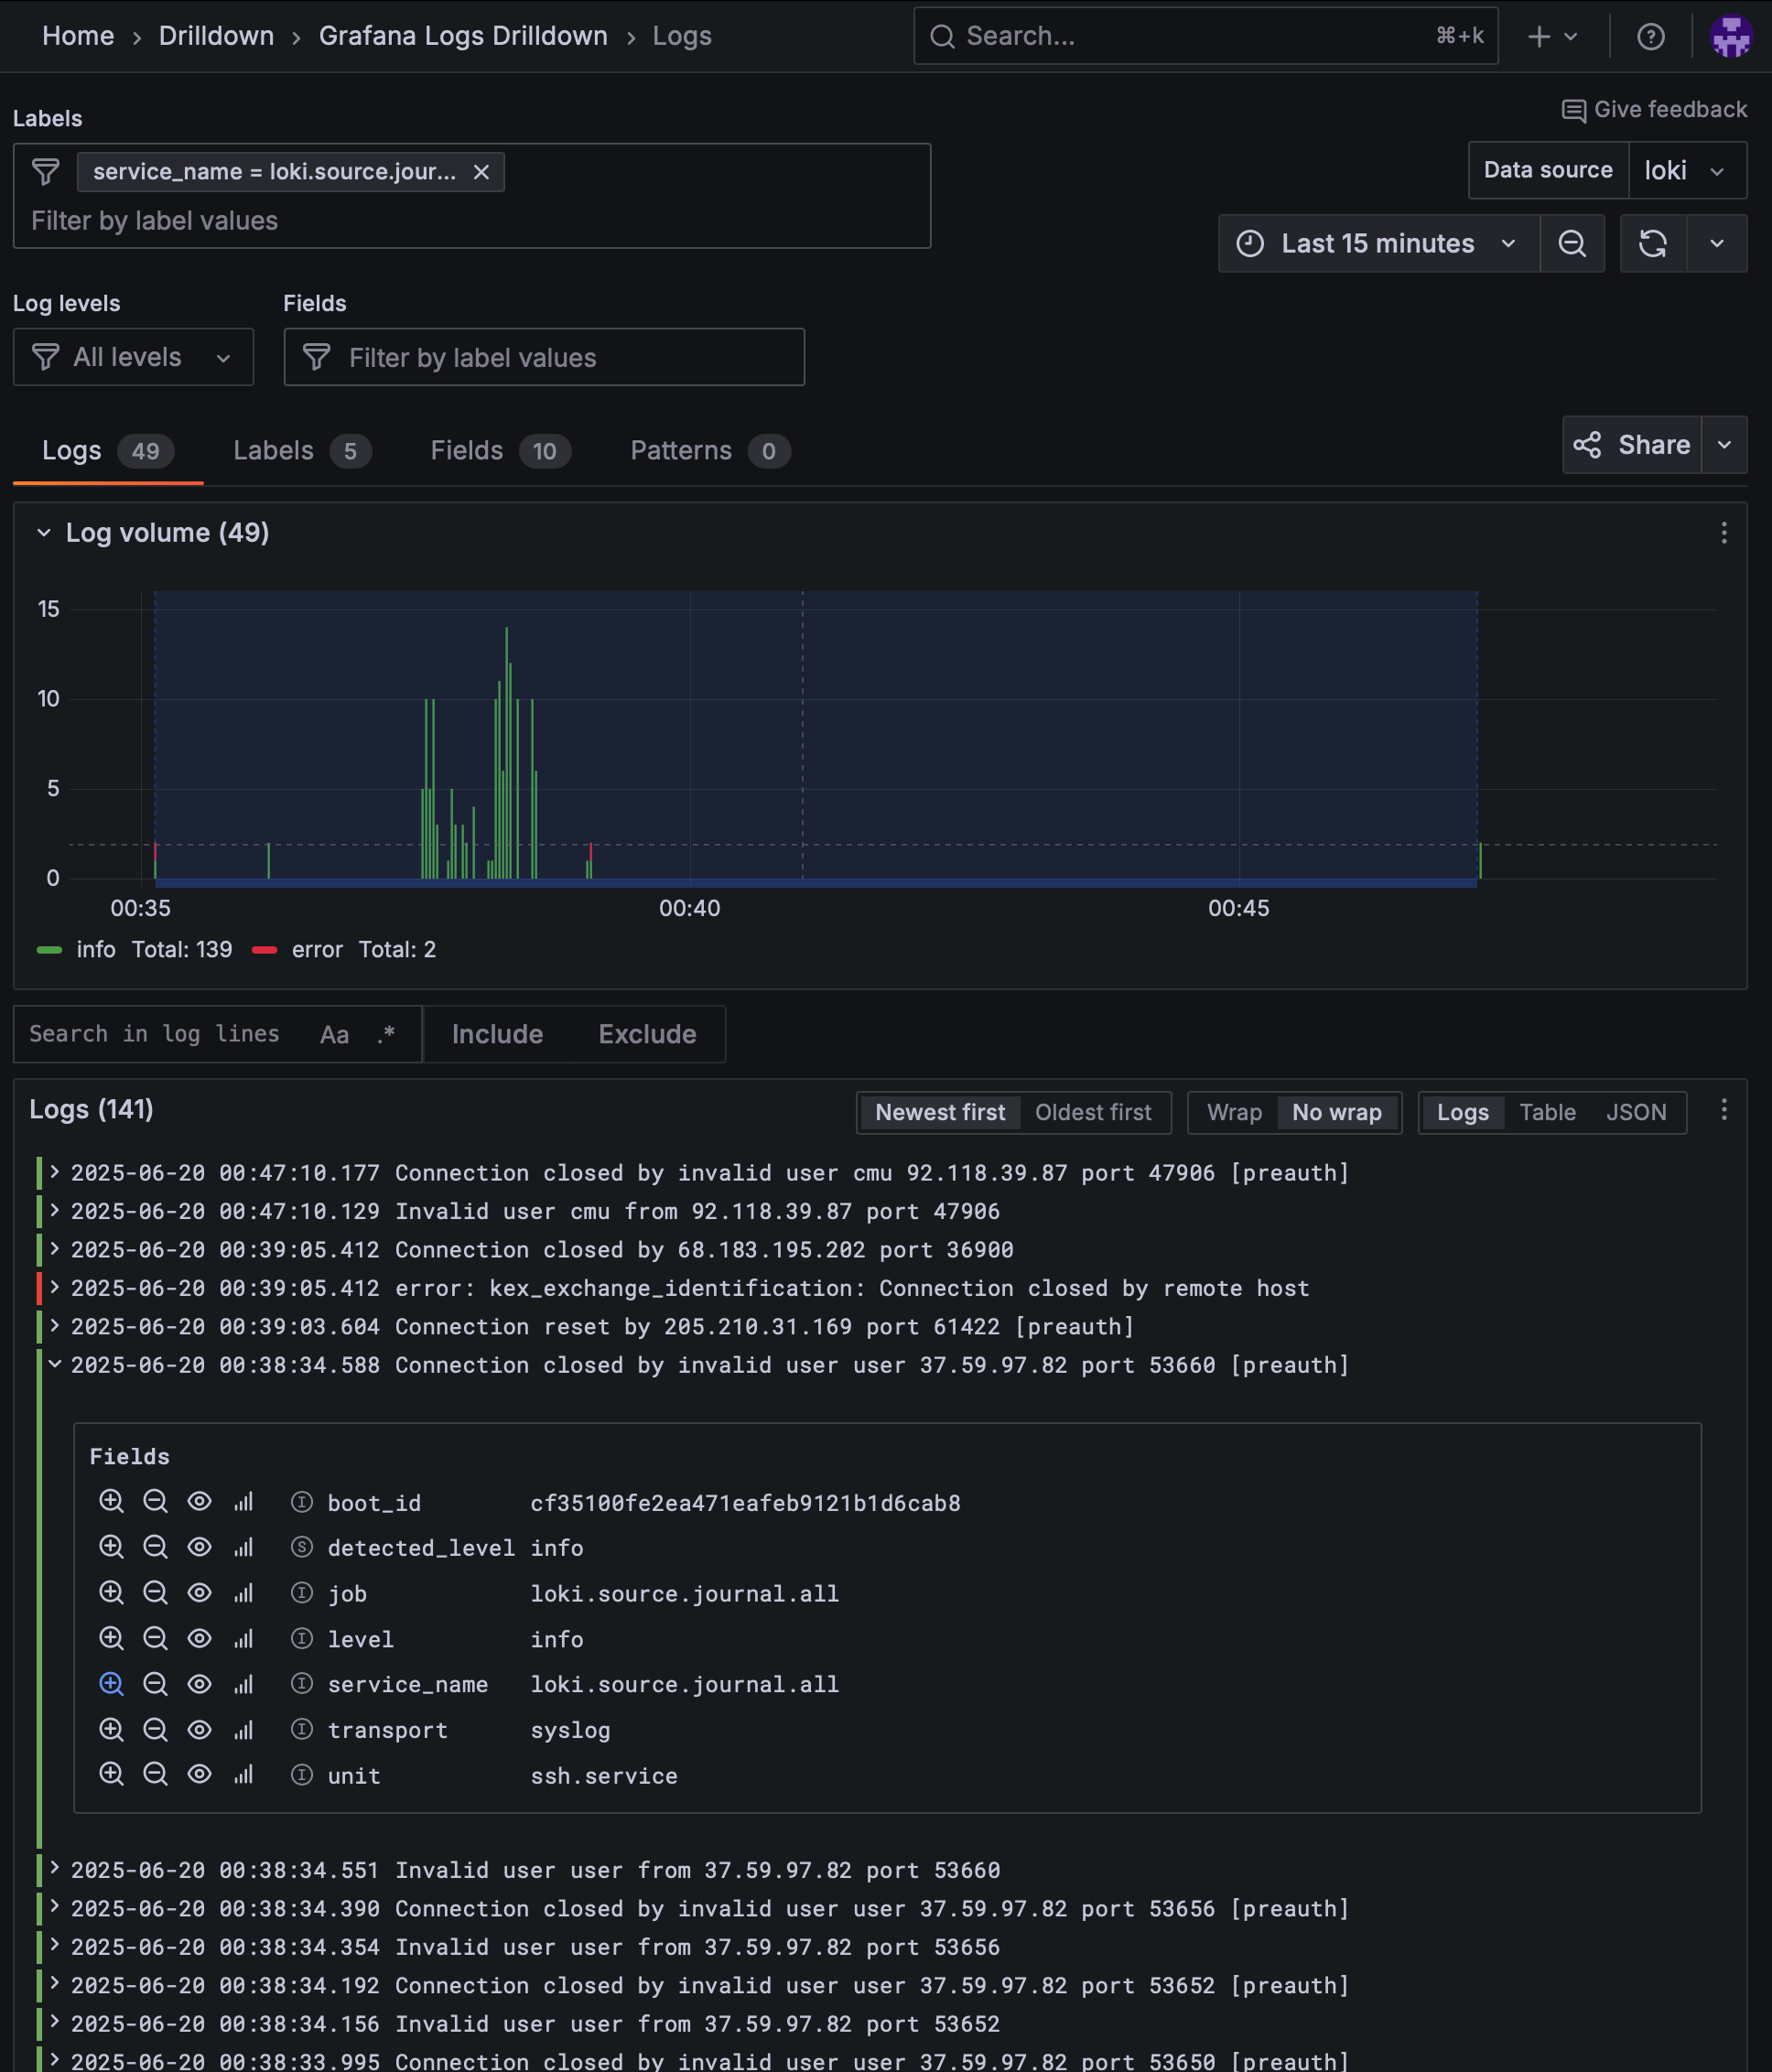
\includegraphics[width=\textwidth]{imaxes/grafana-journal.png}
	\caption{Loki logs in Grafana, showing journal entries with custom labels.}
	\label{fig:grafana-journal}
\end{figure}

\section{Email Server with Mailcow}
\label{sec:mailcow}

Although not discussed in the technology selection chapter, a robust email server is a critical requirement for the new infrastructure, needed for services like Grafana and Passbolt to send alerts and notifications. Mailcow was selected for this role due to its widespread adoption and positive reputation in the open-source self-hosting community. As a complete mail server suite based on Docker, it provides a powerful foundation that will also serve as the Mail Transfer Agent (MTA) for the community's mailing lists, which will be managed by Mailman 3.

\subsection*{Mailcow Container Setup}

To maintain isolation and simplify management, Mailcow is deployed within its own dedicated Incus container. As Mailcow relies on Docker and Docker Compose for its operation, the container needs to be configured to support nested virtualization\cite{incus-faq-docker-nesting}. A new container named \texttt{mailcow} is launched from the Debian 12 image.

\begin{lstlisting}[language=bash,caption={Creating and configuring the Mailcow container.}]
incus launch images:debian/12 mailcow
incus config set mailcow security.nesting=true
incus config set mailcow security.privileged=true
\end{lstlisting}

The \texttt{security.nesting} flag enables the container to run its own containerization environment, while \texttt{security.privileged} is required for Mailcow to manage the networking stack correctly. Inside the container, Docker is installed following the official Docker documentation.

A critical step in deploying an email server on a cloud provider like Hetzner is ensuring that outgoing email ports are not blocked. By default, Hetzner blocks these ports to prevent spam. A support ticket was opened to request the unblocking of these ports for \texttt{gpulux}'s IP address.

To allow external access to Mailcow's services, several ports must be forwarded from the host to the container. This is achieved using Incus proxy devices, which redirect traffic from the host's public IP to the container. Table~\ref{tab:mailcow-ports} lists the required ports.

\begin{table}[H]
    \centering
    \rowcolors{2}{white}{udcgray!25}
    \caption{Ports forwarded to the Mailcow container\cite{mailcow-prerequisites}.}
    \label{tab:mailcow-ports}
    \begin{tabular}{lll}
        \rowcolor{udcpink!25}
        \textbf{Service} & \textbf{Protocol} & \textbf{Port} \\
        \hline
        Postfix SMTP & TCP & 25 \\
        Postfix SMTPS & TCP & 465 \\
        Postfix Submission & TCP & 587 \\
        Dovecot IMAP & TCP & 143 \\
        Dovecot IMAPS & TCP & 993 \\
        Dovecot POP3 & TCP & 110 \\
        Dovecot POP3S & TCP & 995 \\
        Dovecot ManageSieve & TCP & 4190 \\
    \end{tabular}
\end{table}

The commands to create these proxy devices follow a similar pattern as the Caddy proxy setup, created for each port listed in the table. For example, to forward the SMTP port:

\begin{lstlisting}[language=bash,caption={Example of forwarding a port to the Mailcow container.}]
# SMTP (25)
incus config device add mailcow smtp-proxy proxy listen=tcp:0.0.0.0:25 connect=tcp:127.0.0.1:25
\end{lstlisting}

\subsection*{Mailcow Configuration}

After setting up the container and installing Docker, Mailcow is installed by following its official documentation\cite{mailcow-install}. The primary configuration is managed through the \texttt{mailcow.conf} file. Key settings include configuring the server to run behind a reverse proxy\cite{mailcow-reverse-proxy} and disabling IPv6 support to resolve connectivity issues\cite{mailcow-disable-ipv6}. The mail server is configured to run on \texttt{mail.gpulux.org}.

To integrate with the existing monitoring stack, a Prometheus exporter is added to Mailcow's Docker Compose setup. This allows Prometheus to scrape metrics about the mail server's health and performance. The following service definition was added to \texttt{docker\allowbreak-compose.yml}\cite{mailcow-prometheus-exporter}:

\begin{lstlisting}[caption={Docker Compose service for the Mailcow Prometheus exporter.}]
mailcow-exporter:
  image: ghcr.io/mailcow/prometheus-exporter:2
  ports:
    - "9099:9099"
  environment:
    MAILCOW_EXPORTER_HOST: mail.gpulux.org
    MAILCOW_EXPORTER_API_KEY: redacted
  restart: unless-stopped
\end{lstlisting}

Once Mailcow is running, mailboxes for \texttt{grafana@\allowbreak gpulux.org} and \texttt{passbolt@\allowbreak gpulux.org} are created through its web UI. These will be used by the respective services to send email notifications and alerts.

\subsection*{Reverse Proxy Configuration}

To expose Mailcow's web interface and mail autoconfiguration endpoints, the Caddy reverse proxy is configured to forward requests for \texttt{mail.gpulux.org} and its autodiscovery subdomains to the Mailcow container.

\begin{lstlisting}[caption={Caddyfile configuration to reverse proxy Mailcow.}]
mail.gpulux.org autodiscover.mail.gpulux.org autoconfig.mail.gpulux.org {
    reverse_proxy mailcow:80
}
\end{lstlisting}

\section{Password Manager with Passbolt}

The next service to be deployed is Passbolt, the password manager chosen to securely manage credentials for the new infrastructure.

\subsection*{Passbolt Container Setup}

Similar to other services, Passbolt is deployed in a dedicated Incus container named \texttt{passbolt} using a Debian 12 image. No special container configuration was required.

\begin{lstlisting}[language=bash,caption={Creating the Passbolt container.}]
incus launch images:debian/12 passbolt
\end{lstlisting}

\subsection*{Passbolt Configuration}

The installation of Passbolt was performed following the official documentation\cite{passbolt-install-debian}. The process involves adding a dedicated APT repository and installing the \texttt{passbolt-ce-server} package, which triggers a configuration wizard that prompts for database settings.

\begin{lstlisting}[language=bash,caption={Installing Passbolt CE server package.}]
sudo apt install passbolt-ce-server
\end{lstlisting}

Passbolt's package includes Nginx for serving its web interface. However, the existing infrastructure uses a central Caddy instance as a reverse proxy. The automated Nginx setup provided by the Passbolt package was disabled, and manual adjustments were made to its configuration file to ensure compatibility. The key changes involved setting the \texttt{X-Forwarded-Proto} header to ensure that Passbolt generates correct HTTPS URLs when operating behind the proxy.

\begin{lstlisting}[caption={Modified Passbolt Nginx configuration to work behind a reverse proxy.}]
#
#  Passbolt.conf - Nginx configuration file to run the Passbolt software.
#

server {

  listen 80;
  listen [::]:80;

  # Managed by Passbolt
  server_name _;

  set $forwarded_proto $http_x_forwarded_proto; # added this line

  client_body_buffer_size     100K;
  client_header_buffer_size   1K;
  client_max_body_size        5M;

  client_body_timeout   10;
  client_header_timeout 10;
  keepalive_timeout     5 5;
  send_timeout          10;

  root /usr/share/php/passbolt/webroot;
  index index.php;
  error_log /var/log/nginx/passbolt-error.log info;
  access_log /var/log/nginx/passbolt-access.log;

  # Managed by Passbolt
  # include __PASSBOLT_SSL__

  location / {
    try_files $uri $uri/ /index.php?$args;
  }

  location ~ \.php$ {
    try_files                $uri =404;
    include                  fastcgi_params;
    fastcgi_pass             unix:/run/php/php8.2-fpm.sock;
    fastcgi_index            index.php;
    fastcgi_intercept_errors on;
    fastcgi_split_path_info  ^(.+\.php)(.+)$;
    fastcgi_param            SCRIPT_FILENAME $document_root$fastcgi_script_name;
    fastcgi_param            SERVER_NAME $http_host;

    fastcgi_param HTTPS $forwarded_proto; # added this line

    fastcgi_param PHP_VALUE  "upload_max_filesize=5M \n post_max_size=5M";
  }

}
\end{lstlisting}

With the Nginx configuration corrected, accessing \texttt{passbolt.gpulux.org} launches the web-based setup wizard. This final step involves configuring the database connection, generating a GPG key for the server, setting up the SMTP connection to Mailcow, and creating the initial administrator account.

\subsection*{Reverse Proxy Configuration}

To expose Passbolt's web interface, the Caddy reverse proxy is configured to forward requests for \texttt{passbolt.gpulux.org} to the Passbolt container.

\begin{lstlisting}[caption={Caddyfile configuration to reverse proxy Passbolt.}]
passbolt.gpulux.org {
    reverse_proxy passbolt:80
}
\end{lstlisting}

Figure~\ref{fig:passbolt-ui} shows the Passbolt interface after configuration, populated with credentials for other services in the infrastructure.

\begin{figure}[H]
	\centering
	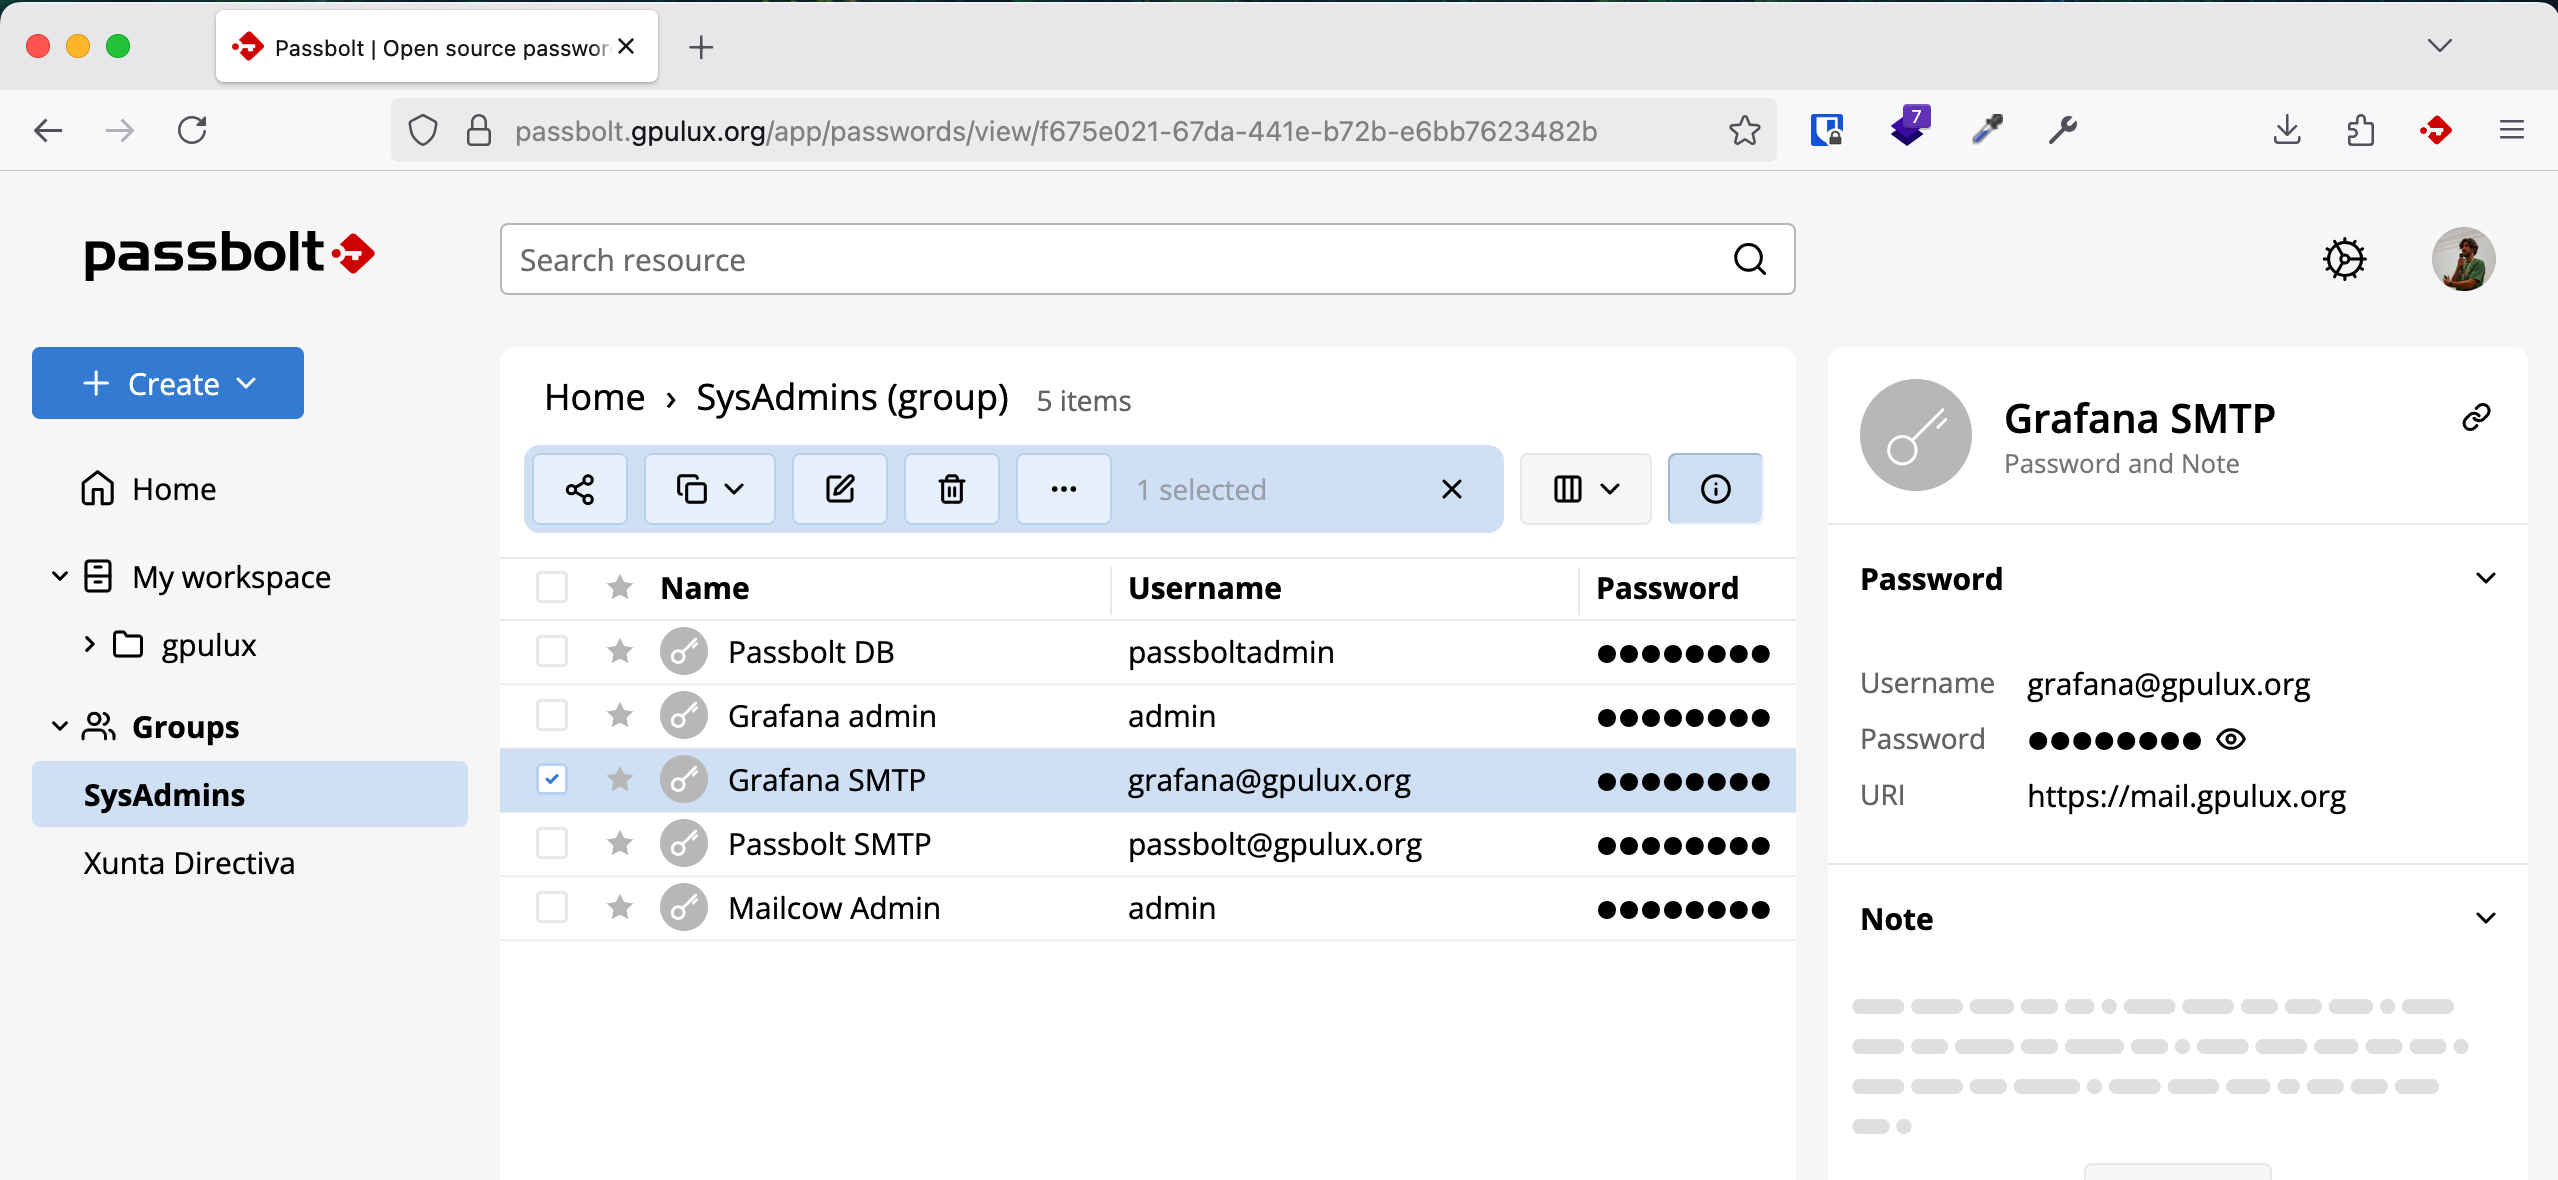
\includegraphics[width=\textwidth]{imaxes/passbolt-gpulux.png}
	\caption{Passbolt web interface showing stored credentials.}
	\label{fig:passbolt-ui}
\end{figure}

  % SPDX-FileCopyrightText: 2025 Laura Milagros Castro Souto <lcastro@udc.es>
%
% SPDX-License-Identifier: GPL-2.0-or-later

\chapter{Conclusións}
\label{chap:conclusions}

\lettrine{D}{erradeiro} capítulo da memoria, onde se presentará a
situación final do traballo, as leccións aprendidas, a relación coas
competencias da titulación en xeral e a mención en particular,
posibles liñas futuras,\dots

\Blindtext


  %%%%%%%%%%%%%%%%%%%%%%%%%%%%%%%%%%%%%%%%
  % Apéndices, glosarios e bibliografía  %
  %%%%%%%%%%%%%%%%%%%%%%%%%%%%%%%%%%%%%%%%

  \appendix
  \appendixpage
  % SPDX-FileCopyrightText: 2025 Emilio José Padrón González <emilio.padron@udc.es>
%
% SPDX-License-Identifier: GPL-2.0-or-later

\chapter{GPUL: +25 Years Freeing Minds}

\lettrine{S}{ince} its founding in September~1998, the Group of Programmers
and Users of Linux (GPUL) has been a driving force for Free Software in A~Coru\~na.
Closely tied to the Faculty of Computer Science at the University of
A Coru\~na, this \gls{glug} began as a student initiative to promote open
standards and the GNU/Linux ecosystem. The original bylaws highlighted
the importance of open development and explicitly named Linux as one of
its key areas of activity. Over time those purely technical objectives
expanded to embrace a strong ethical commitment to the ideals of Free
Software.

From the outset, GPUL adopted four guiding principles, documented in the
minutes of its first board meeting:
\begin{itemize}
  \item Maintain a server accessible through the internet to centralize
    all activities and projects.
  \item Create and sustain mailing lists for internal organization and
    member communication.
  \item Organize short courses, technical talks and trips to major
    community events.
  \item Develop and maintain a website that both disseminates the
    association's work and connects it to the wider community.
\end{itemize}

\section{Origins}

GPUL's roots go back to the Faculty's \gls{bbs}, FiCBBS, which began
operating in 1992. Bulletin Board Systems such as this allowed users to
exchange messages and files via modem long before widespread internet
access. By the mid--1990s a small but enthusiastic group on the
\texttt{fic.linux} area of FiCBBS was experimenting with the early
GNU/Linux distributions, coordinating meetups and even bulk ordering CDs
to ease installation. The momentum of that community culminated in the
formal creation of GPUL in office~0.05 of the Faculty.

Although the founding members were initially focused on the technical
side of Linux, they soon engaged with the broader Free Software
movement. Many became contributors to projects such as Debian and the
Free Software Foundation, and they also set the stage for
Trasno~\cite{Trasno}, the Galician localization community. The group's
history, as well as the contributions of many of its members, is
documented in the video series ``GPUL, historia de un LUG
cualquiera''~\cite{GPULserie}, recorded when the association moved from
its long-standing office to a new shared space.

\section{Infrastructure}

Both FiCBBS and the newborn GPUL initially relied on the Faculty's
University Extension Committee server (CEU) for connectivity. While the
group lacked dedicated hardware, it hosted its first mailing lists there.
Soon a home-built PC, affectionately named \emph{Pule}, became GPUL's
first server. Gradually services such as the website---which started as
static pages and grew into a popular weblog---and the mailing lists were
migrated from CEU to Pule, which eventually obtained its own public IP
address.

Pule was eventually replaced by a more robust machine, \emph{Morpheo},
and later by the association's first cloud-based host, \emph{GPULINO}.
Frequent outages in the newly shared association space motivated the
move to the cloud. A second server, \emph{GPUL\'ON}, soon followed to
reinforce the infrastructure. Over the years numerous services were
deployed on these two hosts, often in an ad-hoc manner. Many were left
without proper maintenance or documentation, leading to an oversized and
outdated infrastructure that is increasingly difficult to sustain.

  %\include{anexos/...}

  \printglossary[type=\acronymtype,title=\nomeglosarioacronimos]
  \printglossary[title=\nomeglosariotermos]

  \bibliographystyle{IEEEtranN}
  \bibliography{\bibconfig,bibliografia/bibliografia}
  \clearpage

\end{document}

%%%%%%%%%%%%%%%%%%%%%%%%%%%%%%%%%%%%%%%%%%%%%%%%%%%%%%%%%%%%%%%%%%%%%%%%%%%%%%%%
